\documentclass[twoside]{book}

% Packages required by doxygen
\usepackage{calc}
\usepackage{doxygen}
\usepackage{graphicx}
\usepackage[utf8]{inputenc}
\usepackage{makeidx}
\usepackage{multicol}
\usepackage{multirow}
\usepackage{textcomp}
\usepackage[table]{xcolor}

% Font selection
\usepackage[T1]{fontenc}
\usepackage{mathptmx}
\usepackage[scaled=.90]{helvet}
\usepackage{courier}
\usepackage{amssymb}
\usepackage{sectsty}
\renewcommand{\familydefault}{\sfdefault}
\allsectionsfont{%
  \fontseries{bc}\selectfont%
  \color{darkgray}%
}
\renewcommand{\DoxyLabelFont}{%
  \fontseries{bc}\selectfont%
  \color{darkgray}%
}

% Page & text layout
\usepackage{geometry}
\geometry{%
  a4paper,%
  top=2.5cm,%
  bottom=2.5cm,%
  left=2.5cm,%
  right=2.5cm%
}
\tolerance=750
\hfuzz=15pt
\hbadness=750
\setlength{\emergencystretch}{15pt}
\setlength{\parindent}{0cm}
\setlength{\parskip}{0.2cm}
\makeatletter
\renewcommand{\paragraph}{%
  \@startsection{paragraph}{4}{0ex}{-1.0ex}{1.0ex}{%
    \normalfont\normalsize\bfseries\SS@parafont%
  }%
}
\renewcommand{\subparagraph}{%
  \@startsection{subparagraph}{5}{0ex}{-1.0ex}{1.0ex}{%
    \normalfont\normalsize\bfseries\SS@subparafont%
  }%
}
\makeatother

% Headers & footers
\usepackage{fancyhdr}
\pagestyle{fancyplain}
\fancyhead[LE]{\fancyplain{}{\bfseries\thepage}}
\fancyhead[CE]{\fancyplain{}{}}
\fancyhead[RE]{\fancyplain{}{\bfseries\leftmark}}
\fancyhead[LO]{\fancyplain{}{\bfseries\rightmark}}
\fancyhead[CO]{\fancyplain{}{}}
\fancyhead[RO]{\fancyplain{}{\bfseries\thepage}}
\fancyfoot[LE]{\fancyplain{}{}}
\fancyfoot[CE]{\fancyplain{}{}}
\fancyfoot[RE]{\fancyplain{}{\bfseries\scriptsize Generated on Fri Jun 9 2017 18\-:34\-:52 for Recast by Doxygen }}
\fancyfoot[LO]{\fancyplain{}{\bfseries\scriptsize Generated on Fri Jun 9 2017 18\-:34\-:52 for Recast by Doxygen }}
\fancyfoot[CO]{\fancyplain{}{}}
\fancyfoot[RO]{\fancyplain{}{}}
\renewcommand{\footrulewidth}{0.4pt}
\renewcommand{\chaptermark}[1]{%
  \markboth{#1}{}%
}
\renewcommand{\sectionmark}[1]{%
  \markright{\thesection\ #1}%
}

% Indices & bibliography
\usepackage{natbib}
\usepackage[titles]{tocloft}
\setcounter{tocdepth}{3}
\setcounter{secnumdepth}{5}
\makeindex

% Hyperlinks (required, but should be loaded last)
\usepackage{ifpdf}
\ifpdf
  \usepackage[pdftex,pagebackref=true]{hyperref}
\else
  \usepackage[ps2pdf,pagebackref=true]{hyperref}
\fi
\hypersetup{%
  colorlinks=true,%
  linkcolor=blue,%
  citecolor=blue,%
  unicode%
}

% Custom commands
\newcommand{\clearemptydoublepage}{%
  \newpage{\pagestyle{empty}\cleardoublepage}%
}


%===== C O N T E N T S =====

\begin{document}

% Titlepage & ToC
\hypersetup{pageanchor=false}
\pagenumbering{roman}
\begin{titlepage}
\vspace*{7cm}
\begin{center}%
{\Large Recast \\[1ex]\large 1 }\\
\vspace*{1cm}
{\large Generated by Doxygen 1.8.6}\\
\vspace*{0.5cm}
{\small Fri Jun 9 2017 18:34:52}\\
\end{center}
\end{titlepage}
\clearemptydoublepage
\tableofcontents
\clearemptydoublepage
\pagenumbering{arabic}
\hypersetup{pageanchor=true}

%--- Begin generated contents ---
\chapter{Main Page}
\label{index}\hypertarget{index}{}Основная идея проекта -\/ не ограничивать игрока в создании заклинаний. Игрок может создавать заклинания, опираясь на физические законы окружающего мира.

\subsection*{Основные концепции проекта\-:}


\begin{DoxyItemize}
\item Проект -\/ игра в жанре R\-P\-G
\item Двумерный игровой мир в представлении пользователя
\item Трёхмерный игровой мир с фиксированной глубиной со стороны логики игры
\item Основной “фишкой” игры является возможность построения -\/ произвольных заклинаний
\item Заклинания строятся в отдельном трёхмерном интерфейсе, управление глубиной на колёсико мыши или wasd+shift+space
\item Заклинания представляют из себя трёхмерные графы, состоящие из узлов и связывающих их рёбер
\item Заклинания завязаны на законах физики и связаны с температурой объектов и кинетикой
\item Создание заклинаний базируется на схемотехнике
\item Приоритет в разработке отдаётся созданию движка создания заклинаний
\item Прототип схож с игрой Terraria
\item Разрушаемый мир
\item Деление мира на тайлы
\end{DoxyItemize}

\subsection*{Примеры заклинаний\-:}


\begin{DoxyItemize}
\item Огненный шар
\item Отталкивание
\end{DoxyItemize}

\subsection*{Документация\-:}

Автоматическая документация генерируется с помощью Doxygen\-: \href{https://glitchless.github.io/Recast/html/}{\tt https\-://glitchless.\-github.\-io/\-Recast/html/}

\subsection*{Клиентская часть\-:}

Репозиторий с игрой на Unity3\-D\-: \href{https://github.com/glitchless/RecastClient}{\tt https\-://github.\-com/glitchless/\-Recast\-Client}

\subsection*{Защита проекта\-:}

Презентация на защите 28 июня 2017 в офисе Mail.\-Ru\-: \href{http://files.reo7sp.ru/recast/presentation.pdf}{\tt http\-://files.\-reo7sp.\-ru/recast/presentation.\-pdf}

\subsection*{Команда \char`\"{}Шкаф Бендера\char`\"{}\-:}


\begin{DoxyItemize}
\item Олег Морозенков
\item Василий Дмитриев
\item Михаил Волынов
\item Юрий Голубев
\item Куликов Никита 
\end{DoxyItemize}
\chapter{Hierarchical Index}
\section{Class Hierarchy}
This inheritance list is sorted roughly, but not completely, alphabetically\-:\begin{DoxyCompactList}
\item \contentsline{section}{crow\-:\-:mustache\-:\-:Action}{\pageref{structcrow_1_1mustache_1_1_action}}{}
\item \contentsline{section}{Catch\-:\-:add\-\_\-const$<$ T $>$}{\pageref{struct_catch_1_1add__const}}{}
\item \contentsline{section}{Catch\-:\-:add\-\_\-lvalue\-\_\-reference$<$ T $>$}{\pageref{struct_catch_1_1add__lvalue__reference}}{}
\item \contentsline{section}{Catch\-:\-:add\-\_\-lvalue\-\_\-reference$<$ T \& $>$}{\pageref{struct_catch_1_1add__lvalue__reference_3_01_t_01_6_01_4}}{}
\item \contentsline{section}{Catch\-:\-:Detail\-:\-:Approx}{\pageref{class_catch_1_1_detail_1_1_approx}}{}
\item \contentsline{section}{crow\-:\-:black\-\_\-magic\-:\-:arguments$<$ Tag $>$}{\pageref{structcrow_1_1black__magic_1_1arguments}}{}
\item \contentsline{section}{crow\-:\-:black\-\_\-magic\-:\-:arguments$<$ 0 $>$}{\pageref{structcrow_1_1black__magic_1_1arguments_3_010_01_4}}{}
\item \contentsline{section}{Catch\-:\-:Assertion\-Info}{\pageref{struct_catch_1_1_assertion_info}}{}
\item \contentsline{section}{Catch\-:\-:Assertion\-Result}{\pageref{class_catch_1_1_assertion_result}}{}
\item \contentsline{section}{Catch\-:\-:Assertion\-Result\-Data}{\pageref{struct_catch_1_1_assertion_result_data}}{}
\item \contentsline{section}{Catch\-:\-:Auto\-Reg}{\pageref{struct_catch_1_1_auto_reg}}{}
\item \contentsline{section}{crow\-:\-:Base\-Rule}{\pageref{classcrow_1_1_base_rule}}{}
\begin{DoxyCompactList}
\item \contentsline{section}{crow\-:\-:Dynamic\-Rule}{\pageref{classcrow_1_1_dynamic_rule}}{}
\item \contentsline{section}{crow\-:\-:Tagged\-Rule$<$ Args $>$}{\pageref{classcrow_1_1_tagged_rule}}{}
\item \contentsline{section}{crow\-:\-:Web\-Socket\-Rule}{\pageref{classcrow_1_1_web_socket_rule}}{}
\end{DoxyCompactList}
\item \contentsline{section}{Catch\-:\-:Detail\-:\-:Borg\-Type}{\pageref{struct_catch_1_1_detail_1_1_borg_type}}{}
\item \contentsline{section}{Bound\-Temperature\-World\-Injector}{\pageref{class_bound_temperature_world_injector}}{}
\item \contentsline{section}{crow\-:\-:detail\-:\-:routing\-\_\-handler\-\_\-call\-\_\-helper\-:\-:call$<$ F, N\-Int, N\-Uint, N\-Double, N\-String, S1, S2 $>$}{\pageref{structcrow_1_1detail_1_1routing__handler__call__helper_1_1call}}{}
\item \contentsline{section}{crow\-:\-:detail\-:\-:routing\-\_\-handler\-\_\-call\-\_\-helper\-:\-:call$<$ F, N\-Int, N\-Uint, N\-Double, N\-String, black\-\_\-magic\-:\-:S$<$ double, Args1...$>$, black\-\_\-magic\-:\-:S$<$ Args2...$>$ $>$}{\pageref{structcrow_1_1detail_1_1routing__handler__call__helper_1_1call_3_01_f_00_01_n_int_00_01_n_uint_0b30fc35e23f441513a63571edf36fc02}}{}
\item \contentsline{section}{crow\-:\-:detail\-:\-:routing\-\_\-handler\-\_\-call\-\_\-helper\-:\-:call$<$ F, N\-Int, N\-Uint, N\-Double, N\-String, black\-\_\-magic\-:\-:S$<$ int64\-\_\-t, Args1...$>$, black\-\_\-magic\-:\-:S$<$ Args2...$>$ $>$}{\pageref{structcrow_1_1detail_1_1routing__handler__call__helper_1_1call_3_01_f_00_01_n_int_00_01_n_uint_0b6a35a476dfcab9d942547331be456a9}}{}
\item \contentsline{section}{crow\-:\-:detail\-:\-:routing\-\_\-handler\-\_\-call\-\_\-helper\-:\-:call$<$ F, N\-Int, N\-Uint, N\-Double, N\-String, black\-\_\-magic\-:\-:S$<$ std\-:\-:string, Args1...$>$, black\-\_\-magic\-:\-:S$<$ Args2...$>$ $>$}{\pageref{structcrow_1_1detail_1_1routing__handler__call__helper_1_1call_3_01_f_00_01_n_int_00_01_n_uint_0d6c3c1bf426d7dfb9e3165c9ff3fd2f3}}{}
\item \contentsline{section}{crow\-:\-:detail\-:\-:routing\-\_\-handler\-\_\-call\-\_\-helper\-:\-:call$<$ F, N\-Int, N\-Uint, N\-Double, N\-String, black\-\_\-magic\-:\-:S$<$ uint64\-\_\-t, Args1...$>$, black\-\_\-magic\-:\-:S$<$ Args2...$>$ $>$}{\pageref{structcrow_1_1detail_1_1routing__handler__call__helper_1_1call_3_01_f_00_01_n_int_00_01_n_uint_00ad4e6269b7fa1968d50bbffd43a8f02}}{}
\item \contentsline{section}{crow\-:\-:detail\-:\-:routing\-\_\-handler\-\_\-call\-\_\-helper\-:\-:call$<$ F, N\-Int, N\-Uint, N\-Double, N\-String, black\-\_\-magic\-:\-:S$<$$>$, black\-\_\-magic\-:\-:S$<$ Args1...$>$ $>$}{\pageref{structcrow_1_1detail_1_1routing__handler__call__helper_1_1call_3_01_f_00_01_n_int_00_01_n_uint_0d7ef20f9a959e64c78052cf52ae9f097}}{}
\item \contentsline{section}{crow\-:\-:detail\-:\-:routing\-\_\-handler\-\_\-call\-\_\-helper\-:\-:call\-\_\-pair$<$ T, Pos $>$}{\pageref{structcrow_1_1detail_1_1routing__handler__call__helper_1_1call__pair}}{}
\item \contentsline{section}{crow\-:\-:detail\-:\-:routing\-\_\-handler\-\_\-call\-\_\-helper\-:\-:call\-\_\-params$<$ H1 $>$}{\pageref{structcrow_1_1detail_1_1routing__handler__call__helper_1_1call__params}}{}
\item \contentsline{section}{crow\-:\-:black\-\_\-magic\-:\-:Call\-Helper$<$ F, Set $>$}{\pageref{structcrow_1_1black__magic_1_1_call_helper}}{}
\item \contentsline{section}{crow\-:\-:black\-\_\-magic\-:\-:Call\-Helper$<$ F, S$<$ Args...$>$ $>$}{\pageref{structcrow_1_1black__magic_1_1_call_helper_3_01_f_00_01_s_3_01_args_8_8_8_4_01_4}}{}
\item \contentsline{section}{Catch\-:\-:Matchers\-:\-:Std\-String\-:\-:Cased\-String}{\pageref{struct_catch_1_1_matchers_1_1_std_string_1_1_cased_string}}{}
\item \contentsline{section}{Catch\-:\-:Case\-Sensitive}{\pageref{struct_catch_1_1_case_sensitive}}{}
\item \contentsline{section}{crow\-:\-:detail\-:\-:check\-\_\-after\-\_\-handle\-\_\-arity\-\_\-3$<$ M\-W $>$}{\pageref{structcrow_1_1detail_1_1check__after__handle__arity__3}}{}
\item \contentsline{section}{crow\-:\-:detail\-:\-:check\-\_\-after\-\_\-handle\-\_\-arity\-\_\-3\-\_\-const$<$ M\-W $>$}{\pageref{structcrow_1_1detail_1_1check__after__handle__arity__3__const}}{}
\item \contentsline{section}{crow\-:\-:detail\-:\-:check\-\_\-before\-\_\-handle\-\_\-arity\-\_\-3$<$ M\-W $>$}{\pageref{structcrow_1_1detail_1_1check__before__handle__arity__3}}{}
\item \contentsline{section}{crow\-:\-:detail\-:\-:check\-\_\-before\-\_\-handle\-\_\-arity\-\_\-3\-\_\-const$<$ M\-W $>$}{\pageref{structcrow_1_1detail_1_1check__before__handle__arity__3__const}}{}
\item \contentsline{section}{crow\-:\-:ci\-\_\-hash}{\pageref{structcrow_1_1ci__hash}}{}
\item \contentsline{section}{crow\-:\-:ci\-\_\-key\-\_\-eq}{\pageref{structcrow_1_1ci__key__eq}}{}
\item \contentsline{section}{Command\-Manager}{\pageref{class_command_manager}}{}
\item \contentsline{section}{Catch\-:\-:Composite\-Generator$<$ T $>$}{\pageref{class_catch_1_1_composite_generator}}{}
\item \contentsline{section}{crow\-:\-:black\-\_\-magic\-:\-:compute\-\_\-parameter\-\_\-tag\-\_\-from\-\_\-args\-\_\-list$<$ Args $>$}{\pageref{structcrow_1_1black__magic_1_1compute__parameter__tag__from__args__list}}{}
\item \contentsline{section}{crow\-:\-:black\-\_\-magic\-:\-:compute\-\_\-parameter\-\_\-tag\-\_\-from\-\_\-args\-\_\-list$<$ Arg, Args...$>$}{\pageref{structcrow_1_1black__magic_1_1compute__parameter__tag__from__args__list_3_01_arg_00_01_args_8_8_8_4}}{}
\item \contentsline{section}{crow\-:\-:black\-\_\-magic\-:\-:compute\-\_\-parameter\-\_\-tag\-\_\-from\-\_\-args\-\_\-list$<$$>$}{\pageref{structcrow_1_1black__magic_1_1compute__parameter__tag__from__args__list_3_4}}{}
\item Concat\begin{DoxyCompactList}
\item \contentsline{section}{crow\-:\-:black\-\_\-magic\-:\-:gen\-\_\-seq$<$ N $>$}{\pageref{structcrow_1_1black__magic_1_1gen__seq}}{}
\end{DoxyCompactList}
\item \contentsline{section}{crow\-:\-:black\-\_\-magic\-:\-:concat$<$ S1, S2 $>$}{\pageref{structcrow_1_1black__magic_1_1concat}}{}
\item \contentsline{section}{Config}{\pageref{class_config}}{}
\item \contentsline{section}{crow\-:\-:websocket\-:\-:connection}{\pageref{structcrow_1_1websocket_1_1connection}}{}
\begin{DoxyCompactList}
\item \contentsline{section}{crow\-:\-:websocket\-:\-:Connection$<$ Adaptor $>$}{\pageref{classcrow_1_1websocket_1_1_connection}}{}
\end{DoxyCompactList}
\item \contentsline{section}{crow\-:\-:Connection$<$ Adaptor, Handler, Middlewares $>$}{\pageref{classcrow_1_1_connection}}{}
\item \contentsline{section}{crow\-:\-:black\-\_\-magic\-:\-:const\-\_\-str}{\pageref{classcrow_1_1black__magic_1_1const__str}}{}
\item context\begin{DoxyCompactList}
\item \contentsline{section}{crow\-:\-:detail\-:\-:partial\-\_\-context$<$ Middlewares $>$}{\pageref{structcrow_1_1detail_1_1partial__context}}{}
\item \contentsline{section}{crow\-:\-:detail\-:\-:partial\-\_\-context$<$ Middlewares...$>$}{\pageref{structcrow_1_1detail_1_1partial__context}}{}
\begin{DoxyCompactList}
\item \contentsline{section}{crow\-:\-:detail\-:\-:context$<$ Middlewares...$>$}{\pageref{structcrow_1_1detail_1_1context}}{}
\item \contentsline{section}{crow\-:\-:detail\-:\-:context$<$ Middlewares $>$}{\pageref{structcrow_1_1detail_1_1context}}{}
\end{DoxyCompactList}
\end{DoxyCompactList}
\item \contentsline{section}{crow\-:\-:Cookie\-Parser\-:\-:context}{\pageref{structcrow_1_1_cookie_parser_1_1context}}{}
\item \contentsline{section}{crow\-:\-:Cookie\-Parser}{\pageref{structcrow_1_1_cookie_parser}}{}
\item \contentsline{section}{Catch\-:\-:Copyable\-Stream}{\pageref{struct_catch_1_1_copyable_stream}}{}
\item \contentsline{section}{Catch\-:\-:Counts}{\pageref{struct_catch_1_1_counts}}{}
\item \contentsline{section}{crow\-:\-:Crow$<$ Middlewares $>$}{\pageref{classcrow_1_1_crow}}{}
\item \contentsline{section}{Catch\-:\-:Decomposed\-Expression}{\pageref{struct_catch_1_1_decomposed_expression}}{}
\begin{DoxyCompactList}
\item \contentsline{section}{Catch\-:\-:Binary\-Expression$<$ Lhs\-T, Op, Rhs\-T $>$}{\pageref{class_catch_1_1_binary_expression}}{}
\item \contentsline{section}{Catch\-:\-:Expression\-Lhs$<$ T $>$}{\pageref{class_catch_1_1_expression_lhs}}{}
\item \contentsline{section}{Catch\-:\-:Match\-Expression$<$ Arg\-T, Matcher\-T $>$}{\pageref{class_catch_1_1_match_expression}}{}
\item \contentsline{section}{Catch\-:\-:Result\-Builder}{\pageref{class_catch_1_1_result_builder}}{}
\end{DoxyCompactList}
\item \contentsline{section}{crow\-:\-:detail\-:\-:dumb\-\_\-timer\-\_\-queue}{\pageref{classcrow_1_1detail_1_1dumb__timer__queue}}{}
\item \contentsline{section}{crow\-:\-:black\-\_\-magic\-:\-:empty\-\_\-context$<$ T $>$}{\pageref{structcrow_1_1black__magic_1_1empty__context}}{}
\item equality\-\_\-comparable\begin{DoxyCompactList}
\item \contentsline{section}{crow\-:\-:json\-:\-:detail\-:\-:r\-\_\-string}{\pageref{structcrow_1_1json_1_1detail_1_1r__string}}{}
\item \contentsline{section}{crow\-:\-:json\-:\-:detail\-:\-:r\-\_\-string}{\pageref{structcrow_1_1json_1_1detail_1_1r__string}}{}
\end{DoxyCompactList}
\item \contentsline{section}{Catch\-:\-:Internal\-:\-:Evaluator$<$ T1, T2, Op $>$}{\pageref{class_catch_1_1_internal_1_1_evaluator}}{}
\item \contentsline{section}{Catch\-:\-:Internal\-:\-:Evaluator$<$ T1, T2, Is\-Equal\-To $>$}{\pageref{struct_catch_1_1_internal_1_1_evaluator_3_01_t1_00_01_t2_00_01_is_equal_to_01_4}}{}
\item \contentsline{section}{Catch\-:\-:Internal\-:\-:Evaluator$<$ T1, T2, Is\-Greater\-Than $>$}{\pageref{struct_catch_1_1_internal_1_1_evaluator_3_01_t1_00_01_t2_00_01_is_greater_than_01_4}}{}
\item \contentsline{section}{Catch\-:\-:Internal\-:\-:Evaluator$<$ T1, T2, Is\-Greater\-Than\-Or\-Equal\-To $>$}{\pageref{struct_catch_1_1_internal_1_1_evaluator_3_01_t1_00_01_t2_00_01_is_greater_than_or_equal_to_01_4}}{}
\item \contentsline{section}{Catch\-:\-:Internal\-:\-:Evaluator$<$ T1, T2, Is\-Less\-Than $>$}{\pageref{struct_catch_1_1_internal_1_1_evaluator_3_01_t1_00_01_t2_00_01_is_less_than_01_4}}{}
\item \contentsline{section}{Catch\-:\-:Internal\-:\-:Evaluator$<$ T1, T2, Is\-Less\-Than\-Or\-Equal\-To $>$}{\pageref{struct_catch_1_1_internal_1_1_evaluator_3_01_t1_00_01_t2_00_01_is_less_than_or_equal_to_01_4}}{}
\item \contentsline{section}{Catch\-:\-:Internal\-:\-:Evaluator$<$ T1, T2, Is\-Not\-Equal\-To $>$}{\pageref{struct_catch_1_1_internal_1_1_evaluator_3_01_t1_00_01_t2_00_01_is_not_equal_to_01_4}}{}
\item exception\begin{DoxyCompactList}
\item \contentsline{section}{Catch\-:\-:Not\-Implemented\-Exception}{\pageref{class_catch_1_1_not_implemented_exception}}{}
\item \contentsline{section}{crow\-:\-:mustache\-:\-:invalid\-\_\-template\-\_\-exception}{\pageref{classcrow_1_1mustache_1_1invalid__template__exception}}{}
\item \contentsline{section}{Invalid\-Login\-Or\-Password}{\pageref{class_invalid_login_or_password}}{}
\item \contentsline{section}{Server\-Full\-Exception}{\pageref{class_server_full_exception}}{}
\end{DoxyCompactList}
\item \contentsline{section}{Catch\-:\-:Exception\-Translator\-Registrar}{\pageref{class_catch_1_1_exception_translator_registrar}}{}
\item false\-\_\-type\begin{DoxyCompactList}
\item \contentsline{section}{crow\-:\-:black\-\_\-magic\-:\-:contains$<$ Tp $>$}{\pageref{structcrow_1_1black__magic_1_1contains_3_01_tp_01_4}}{}
\end{DoxyCompactList}
\item \contentsline{section}{Catch\-:\-:Detail\-:\-:False\-Type}{\pageref{struct_catch_1_1_detail_1_1_false_type}}{}
\item \contentsline{section}{crow\-:\-:utility\-:\-:function\-\_\-traits$<$ T $>$}{\pageref{structcrow_1_1utility_1_1function__traits}}{}
\item \contentsline{section}{crow\-:\-:utility\-:\-:function\-\_\-traits$<$ R(Class\-Type\-:\-:$\ast$)(Args...) const $>$}{\pageref{structcrow_1_1utility_1_1function__traits_3_01_r_07_class_type_1_1_5_08_07_args_8_8_8_08_01const_01_01_4}}{}
\item \contentsline{section}{crow\-:\-:utility\-:\-:function\-\_\-traits$<$ R(Class\-Type\-:\-:$\ast$)(Args...)$>$}{\pageref{structcrow_1_1utility_1_1function__traits_3_01_r_07_class_type_1_1_5_08_07_args_8_8_8_08_4}}{}
\item \contentsline{section}{crow\-:\-:utility\-:\-:function\-\_\-traits$<$ std\-:\-:function$<$ R(Args...)$>$ $>$}{\pageref{structcrow_1_1utility_1_1function__traits_3_01std_1_1function_3_01_r_07_args_8_8_8_08_4_01_4}}{}
\item \contentsline{section}{Generic\-Scalar$<$ T $>$}{\pageref{struct_generic_scalar}}{}
\item \contentsline{section}{Generic\-Scalar$<$ int $>$}{\pageref{struct_generic_scalar}}{}
\begin{DoxyCompactList}
\item \contentsline{section}{Coord}{\pageref{struct_coord}}{}
\item \contentsline{section}{Size}{\pageref{struct_size}}{}
\item \contentsline{section}{Temperature}{\pageref{struct_temperature}}{}
\end{DoxyCompactList}
\item \contentsline{section}{crow\-:\-:detail\-:\-:check\-\_\-before\-\_\-handle\-\_\-arity\-\_\-3\-\_\-const$<$ M\-W $>$\-:\-:get$<$ T, const $>$}{\pageref{structcrow_1_1detail_1_1check__before__handle__arity__3__const_1_1get}}{}
\item \contentsline{section}{crow\-:\-:detail\-:\-:check\-\_\-before\-\_\-handle\-\_\-arity\-\_\-3$<$ M\-W $>$\-:\-:get$<$ T, $>$}{\pageref{structcrow_1_1detail_1_1check__before__handle__arity__3_1_1get}}{}
\item \contentsline{section}{crow\-:\-:detail\-:\-:check\-\_\-after\-\_\-handle\-\_\-arity\-\_\-3\-\_\-const$<$ M\-W $>$\-:\-:get$<$ T, const $>$}{\pageref{structcrow_1_1detail_1_1check__after__handle__arity__3__const_1_1get}}{}
\item \contentsline{section}{crow\-:\-:detail\-:\-:check\-\_\-after\-\_\-handle\-\_\-arity\-\_\-3$<$ M\-W $>$\-:\-:get$<$ T, $>$}{\pageref{structcrow_1_1detail_1_1check__after__handle__arity__3_1_1get}}{}
\item \contentsline{section}{crow\-:\-:detail\-:\-:get\-\_\-index\-\_\-of\-\_\-element\-\_\-from\-\_\-tuple\-\_\-by\-\_\-type\-\_\-impl$<$ T, N, Args $>$}{\pageref{structcrow_1_1detail_1_1get__index__of__element__from__tuple__by__type__impl}}{}
\item \contentsline{section}{crow\-:\-:detail\-:\-:get\-\_\-index\-\_\-of\-\_\-element\-\_\-from\-\_\-tuple\-\_\-by\-\_\-type\-\_\-impl$<$ T, N, T, Args...$>$}{\pageref{structcrow_1_1detail_1_1get__index__of__element__from__tuple__by__type__impl_3_01_t_00_01_n_00_01_t_00_01_args_8_8_8_4}}{}
\item \contentsline{section}{crow\-:\-:detail\-:\-:get\-\_\-index\-\_\-of\-\_\-element\-\_\-from\-\_\-tuple\-\_\-by\-\_\-type\-\_\-impl$<$ T, N, U, Args...$>$}{\pageref{structcrow_1_1detail_1_1get__index__of__element__from__tuple__by__type__impl_3_01_t_00_01_n_00_01_u_00_01_args_8_8_8_4}}{}
\item \contentsline{section}{crow\-:\-:detail\-:\-:routing\-\_\-handler\-\_\-call\-\_\-helper\-:\-:Wrapped$<$ Func, Args\-Wrapped $>$\-:\-:handler\-\_\-type\-\_\-helper$<$ Args $>$}{\pageref{structcrow_1_1detail_1_1routing__handler__call__helper_1_1_wrapped_1_1handler__type__helper}}{}
\item \contentsline{section}{crow\-:\-:detail\-:\-:routing\-\_\-handler\-\_\-call\-\_\-helper\-:\-:Wrapped$<$ Func, Args\-Wrapped $>$\-:\-:handler\-\_\-type\-\_\-helper$<$ Args\-Wrapped...$>$}{\pageref{structcrow_1_1detail_1_1routing__handler__call__helper_1_1_wrapped_1_1handler__type__helper}}{}
\item \contentsline{section}{crow\-:\-:detail\-:\-:routing\-\_\-handler\-\_\-call\-\_\-helper\-:\-:Wrapped$<$ Func, Args\-Wrapped $>$\-:\-:handler\-\_\-type\-\_\-helper$<$ const request \&, Args...$>$}{\pageref{structcrow_1_1detail_1_1routing__handler__call__helper_1_1_wrapped_1_1handler__type__helper_3_01176bac6491f2834cd36a05c30aa75bc3}}{}
\item \contentsline{section}{crow\-:\-:detail\-:\-:routing\-\_\-handler\-\_\-call\-\_\-helper\-:\-:Wrapped$<$ Func, Args\-Wrapped $>$\-:\-:handler\-\_\-type\-\_\-helper$<$ const request \&, response \&, Args...$>$}{\pageref{structcrow_1_1detail_1_1routing__handler__call__helper_1_1_wrapped_1_1handler__type__helper_3_01506e35faa94646c63b5476ce8ce1df0a}}{}
\item \contentsline{section}{http\-\_\-parser}{\pageref{structhttp__parser}}{}
\begin{DoxyCompactList}
\item \contentsline{section}{crow\-:\-:H\-T\-T\-P\-Parser$<$ Handler $>$}{\pageref{structcrow_1_1_h_t_t_p_parser}}{}
\item \contentsline{section}{crow\-:\-:H\-T\-T\-P\-Parser$<$ crow\-:\-:Connection $>$}{\pageref{structcrow_1_1_h_t_t_p_parser}}{}
\end{DoxyCompactList}
\item \contentsline{section}{http\-\_\-parser\-\_\-settings}{\pageref{structhttp__parser__settings}}{}
\item \contentsline{section}{http\-\_\-parser\-\_\-url}{\pageref{structhttp__parser__url}}{}
\item \contentsline{section}{I\-Command}{\pageref{class_i_command}}{}
\begin{DoxyCompactList}
\item \contentsline{section}{Stop\-Command}{\pageref{class_stop_command}}{}
\end{DoxyCompactList}
\item \contentsline{section}{I\-Command\-Sender}{\pageref{class_i_command_sender}}{}
\begin{DoxyCompactList}
\item \contentsline{section}{Server}{\pageref{class_server}}{}
\end{DoxyCompactList}
\item \contentsline{section}{Catch\-:\-:I\-Context}{\pageref{struct_catch_1_1_i_context}}{}
\begin{DoxyCompactList}
\item \contentsline{section}{Catch\-:\-:I\-Mutable\-Context}{\pageref{struct_catch_1_1_i_mutable_context}}{}
\end{DoxyCompactList}
\item \contentsline{section}{I\-Event}{\pageref{class_i_event}}{}
\begin{DoxyCompactList}
\item \contentsline{section}{Heat\-Event}{\pageref{class_heat_event}}{}
\end{DoxyCompactList}
\item \contentsline{section}{I\-Event\-Listener}{\pageref{class_i_event_listener}}{}
\begin{DoxyCompactList}
\item \contentsline{section}{Spell\-Event\-Listener}{\pageref{class_spell_event_listener}}{}
\end{DoxyCompactList}
\item \contentsline{section}{Catch\-:\-:I\-Exception\-Translator}{\pageref{struct_catch_1_1_i_exception_translator}}{}
\item \contentsline{section}{Catch\-:\-:I\-Exception\-Translator\-Registry}{\pageref{struct_catch_1_1_i_exception_translator_registry}}{}
\item \contentsline{section}{Catch\-:\-:I\-Generator$<$ T $>$}{\pageref{struct_catch_1_1_i_generator}}{}
\begin{DoxyCompactList}
\item \contentsline{section}{Catch\-:\-:Between\-Generator$<$ T $>$}{\pageref{class_catch_1_1_between_generator}}{}
\item \contentsline{section}{Catch\-:\-:Values\-Generator$<$ T $>$}{\pageref{class_catch_1_1_values_generator}}{}
\end{DoxyCompactList}
\item \contentsline{section}{Catch\-:\-:I\-Generator\-Info}{\pageref{struct_catch_1_1_i_generator_info}}{}
\item \contentsline{section}{Catch\-:\-:I\-Generators\-For\-Test}{\pageref{struct_catch_1_1_i_generators_for_test}}{}
\item \contentsline{section}{crow\-:\-:I\-Log\-Handler}{\pageref{classcrow_1_1_i_log_handler}}{}
\begin{DoxyCompactList}
\item \contentsline{section}{crow\-:\-:Cerr\-Log\-Handler}{\pageref{classcrow_1_1_cerr_log_handler}}{}
\end{DoxyCompactList}
\item \contentsline{section}{Catch\-:\-:I\-Mutable\-Registry\-Hub}{\pageref{struct_catch_1_1_i_mutable_registry_hub}}{}
\item \contentsline{section}{Input\-Thread}{\pageref{class_input_thread}}{}
\item \contentsline{section}{Int\-Scale}{\pageref{struct_int_scale}}{}
\item \contentsline{section}{Int\-Scale\-Parallelepiped}{\pageref{struct_int_scale_parallelepiped}}{}
\item \contentsline{section}{Catch\-:\-:I\-Registry\-Hub}{\pageref{struct_catch_1_1_i_registry_hub}}{}
\item \contentsline{section}{Catch\-:\-:I\-Result\-Capture}{\pageref{struct_catch_1_1_i_result_capture}}{}
\item \contentsline{section}{Catch\-:\-:I\-Runner}{\pageref{struct_catch_1_1_i_runner}}{}
\item \contentsline{section}{crow\-:\-:detail\-:\-:is\-\_\-after\-\_\-handle\-\_\-arity\-\_\-3\-\_\-impl$<$ T $>$}{\pageref{structcrow_1_1detail_1_1is__after__handle__arity__3__impl}}{}
\item \contentsline{section}{crow\-:\-:detail\-:\-:is\-\_\-before\-\_\-handle\-\_\-arity\-\_\-3\-\_\-impl$<$ T $>$}{\pageref{structcrow_1_1detail_1_1is__before__handle__arity__3__impl}}{}
\item \contentsline{section}{I\-Serializable}{\pageref{class_i_serializable}}{}
\item \contentsline{section}{Catch\-:\-:Detail\-:\-:Is\-Stream\-Insertable$<$ T $>$}{\pageref{struct_catch_1_1_detail_1_1_is_stream_insertable}}{}
\item \contentsline{section}{Catch\-:\-:I\-Tag\-Alias\-Registry}{\pageref{struct_catch_1_1_i_tag_alias_registry}}{}
\item \contentsline{section}{I\-Temperature\-World}{\pageref{class_i_temperature_world}}{}
\begin{DoxyCompactList}
\item \contentsline{section}{I\-Temperature\-World\-Boundable$<$ I\-Temperature\-World $>$}{\pageref{class_i_temperature_world_boundable}}{}
\begin{DoxyCompactList}
\item \contentsline{section}{Bound\-Temperature\-World}{\pageref{class_bound_temperature_world}}{}
\begin{DoxyCompactList}
\item \contentsline{section}{I\-Temperature\-World\-Scalable$<$ Bound\-Temperature\-World $>$}{\pageref{class_i_temperature_world_scalable}}{}
\begin{DoxyCompactList}
\item \contentsline{section}{I\-Temperature\-World\-Scalable\-Mutable$<$ I\-Temperature\-World\-Scalable$<$ Bound\-Temperature\-World $>$ $>$}{\pageref{class_i_temperature_world_scalable_mutable}}{}
\begin{DoxyCompactList}
\item \contentsline{section}{Scalable\-Bound\-Temperature\-World}{\pageref{class_scalable_bound_temperature_world}}{}
\end{DoxyCompactList}
\end{DoxyCompactList}
\end{DoxyCompactList}
\end{DoxyCompactList}
\item \contentsline{section}{I\-Temperature\-World\-Chunkable$<$ I\-Temperature\-World $>$}{\pageref{class_i_temperature_world_chunkable}}{}
\begin{DoxyCompactList}
\item \contentsline{section}{I\-Temperature\-World\-Chunkable\-Mutable$<$ I\-Temperature\-World\-Chunkable$<$ I\-Temperature\-World $>$ $>$}{\pageref{class_i_temperature_world_chunkable_mutable}}{}
\begin{DoxyCompactList}
\item \contentsline{section}{Chunked\-Temperature\-World}{\pageref{class_chunked_temperature_world}}{}
\begin{DoxyCompactList}
\item \contentsline{section}{Generatable\-Chunked\-Temperature\-World}{\pageref{class_generatable_chunked_temperature_world}}{}
\begin{DoxyCompactList}
\item \contentsline{section}{Scaling\-Generatable\-Chunked\-Temperature\-World}{\pageref{class_scaling_generatable_chunked_temperature_world}}{}
\end{DoxyCompactList}
\end{DoxyCompactList}
\item \contentsline{section}{I\-Temperature\-World\-Chunkable\-Generatable$<$ I\-Temperature\-World\-Chunkable\-Mutable$<$ I\-Temperature\-World\-Chunkable$<$ I\-Temperature\-World $>$ $>$ $>$}{\pageref{class_i_temperature_world_chunkable_generatable}}{}
\begin{DoxyCompactList}
\item \contentsline{section}{I\-Temperature\-World\-Chunkable\-Observable$<$ I\-Temperature\-World\-Chunkable\-Generatable$<$ I\-Temperature\-World\-Chunkable\-Mutable$<$ I\-Temperature\-World\-Chunkable$<$ I\-Temperature\-World $>$ $>$ $>$ $>$}{\pageref{class_i_temperature_world_chunkable_observable}}{}
\begin{DoxyCompactList}
\item \contentsline{section}{Generatable\-Chunked\-Temperature\-World}{\pageref{class_generatable_chunked_temperature_world}}{}
\item \contentsline{section}{I\-Temperature\-World\-Point\-Prioritizable$<$ I\-Temperature\-World\-Chunkable\-Observable$<$ I\-Temperature\-World\-Chunkable\-Generatable$<$ I\-Temperature\-World\-Chunkable\-Mutable$<$ I\-Temperature\-World\-Chunkable$<$ I\-Temperature\-World $>$ $>$ $>$ $>$ $>$}{\pageref{class_i_temperature_world_point_prioritizable}}{}
\item \contentsline{section}{Scaling\-Generatable\-Chunked\-Temperature\-World}{\pageref{class_scaling_generatable_chunked_temperature_world}}{}
\end{DoxyCompactList}
\end{DoxyCompactList}
\end{DoxyCompactList}
\end{DoxyCompactList}
\end{DoxyCompactList}
\item \contentsline{section}{I\-Temperature\-World\-Boundable\-Mixin}{\pageref{class_i_temperature_world_boundable_mixin}}{}
\begin{DoxyCompactList}
\item \contentsline{section}{I\-Temperature\-World\-Boundable$<$ T $>$}{\pageref{class_i_temperature_world_boundable}}{}
\item \contentsline{section}{I\-Temperature\-World\-Boundable$<$ I\-Temperature\-World $>$}{\pageref{class_i_temperature_world_boundable}}{}
\end{DoxyCompactList}
\item \contentsline{section}{I\-Temperature\-World\-Chunkable\-Generatable\-Mixin}{\pageref{class_i_temperature_world_chunkable_generatable_mixin}}{}
\begin{DoxyCompactList}
\item \contentsline{section}{I\-Temperature\-World\-Chunkable\-Generatable$<$ T $>$}{\pageref{class_i_temperature_world_chunkable_generatable}}{}
\item \contentsline{section}{I\-Temperature\-World\-Chunkable\-Generatable$<$ I\-Temperature\-World\-Chunkable\-Mutable$<$ I\-Temperature\-World\-Chunkable$<$ I\-Temperature\-World $>$ $>$ $>$}{\pageref{class_i_temperature_world_chunkable_generatable}}{}
\end{DoxyCompactList}
\item \contentsline{section}{I\-Temperature\-World\-Chunkable\-Mixin}{\pageref{class_i_temperature_world_chunkable_mixin}}{}
\begin{DoxyCompactList}
\item \contentsline{section}{I\-Temperature\-World\-Chunkable$<$ T $>$}{\pageref{class_i_temperature_world_chunkable}}{}
\item \contentsline{section}{I\-Temperature\-World\-Chunkable$<$ I\-Temperature\-World $>$}{\pageref{class_i_temperature_world_chunkable}}{}
\end{DoxyCompactList}
\item \contentsline{section}{I\-Temperature\-World\-Chunkable\-Mutable\-Mixin}{\pageref{class_i_temperature_world_chunkable_mutable_mixin}}{}
\begin{DoxyCompactList}
\item \contentsline{section}{I\-Temperature\-World\-Chunkable\-Mutable$<$ T $>$}{\pageref{class_i_temperature_world_chunkable_mutable}}{}
\item \contentsline{section}{I\-Temperature\-World\-Chunkable\-Mutable$<$ I\-Temperature\-World\-Chunkable$<$ I\-Temperature\-World $>$ $>$}{\pageref{class_i_temperature_world_chunkable_mutable}}{}
\end{DoxyCompactList}
\item \contentsline{section}{I\-Temperature\-World\-Chunkable\-Observable\-Mixin}{\pageref{class_i_temperature_world_chunkable_observable_mixin}}{}
\begin{DoxyCompactList}
\item \contentsline{section}{I\-Temperature\-World\-Chunkable\-Observable$<$ T $>$}{\pageref{class_i_temperature_world_chunkable_observable}}{}
\item \contentsline{section}{I\-Temperature\-World\-Chunkable\-Observable$<$ I\-Temperature\-World\-Chunkable\-Generatable$<$ I\-Temperature\-World\-Chunkable\-Mutable$<$ I\-Temperature\-World\-Chunkable$<$ I\-Temperature\-World $>$ $>$ $>$ $>$}{\pageref{class_i_temperature_world_chunkable_observable}}{}
\end{DoxyCompactList}
\item \contentsline{section}{I\-Temperature\-World\-Point\-Prioritizable\-Mixin}{\pageref{class_i_temperature_world_point_prioritizable_mixin}}{}
\begin{DoxyCompactList}
\item \contentsline{section}{I\-Temperature\-World\-Point\-Prioritizable$<$ T $>$}{\pageref{class_i_temperature_world_point_prioritizable}}{}
\item \contentsline{section}{I\-Temperature\-World\-Point\-Prioritizable$<$ I\-Temperature\-World\-Chunkable\-Observable$<$ I\-Temperature\-World\-Chunkable\-Generatable$<$ I\-Temperature\-World\-Chunkable\-Mutable$<$ I\-Temperature\-World\-Chunkable$<$ I\-Temperature\-World $>$ $>$ $>$ $>$ $>$}{\pageref{class_i_temperature_world_point_prioritizable}}{}
\end{DoxyCompactList}
\item \contentsline{section}{I\-Temperature\-World\-Scalable\-Mixin}{\pageref{class_i_temperature_world_scalable_mixin}}{}
\begin{DoxyCompactList}
\item \contentsline{section}{I\-Temperature\-World\-Scalable$<$ T $>$}{\pageref{class_i_temperature_world_scalable}}{}
\item \contentsline{section}{I\-Temperature\-World\-Scalable$<$ Bound\-Temperature\-World $>$}{\pageref{class_i_temperature_world_scalable}}{}
\end{DoxyCompactList}
\item \contentsline{section}{I\-Temperature\-World\-Scalable\-Mutable\-Mixin}{\pageref{class_i_temperature_world_scalable_mutable_mixin}}{}
\begin{DoxyCompactList}
\item \contentsline{section}{I\-Temperature\-World\-Scalable\-Mutable$<$ T $>$}{\pageref{class_i_temperature_world_scalable_mutable}}{}
\item \contentsline{section}{I\-Temperature\-World\-Scalable\-Mutable$<$ I\-Temperature\-World\-Scalable$<$ Bound\-Temperature\-World $>$ $>$}{\pageref{class_i_temperature_world_scalable_mutable}}{}
\end{DoxyCompactList}
\item \contentsline{section}{Catch\-:\-:I\-Test\-Case\-Registry}{\pageref{struct_catch_1_1_i_test_case_registry}}{}
\item \contentsline{section}{I\-Timer}{\pageref{class_i_timer}}{}
\begin{DoxyCompactList}
\item \contentsline{section}{Basic\-Timer}{\pageref{class_basic_timer}}{}
\item \contentsline{section}{I\-Timer\-Blockable$<$ I\-Timer $>$}{\pageref{class_i_timer_blockable}}{}
\begin{DoxyCompactList}
\item \contentsline{section}{Synchronized\-Blocking\-Timer}{\pageref{class_synchronized_blocking_timer}}{}
\end{DoxyCompactList}
\end{DoxyCompactList}
\item \contentsline{section}{I\-Timer\-Blockable\-Mixin}{\pageref{class_i_timer_blockable_mixin}}{}
\begin{DoxyCompactList}
\item \contentsline{section}{I\-Timer\-Blockable$<$ T $>$}{\pageref{class_i_timer_blockable}}{}
\item \contentsline{section}{I\-Timer\-Blockable$<$ I\-Timer $>$}{\pageref{class_i_timer_blockable}}{}
\end{DoxyCompactList}
\item \contentsline{section}{I\-Updater}{\pageref{class_i_updater}}{}
\begin{DoxyCompactList}
\item \contentsline{section}{Average\-Share\-Temperature\-World\-Updater}{\pageref{class_average_share_temperature_world_updater}}{}
\item \contentsline{section}{Threaded\-Chunked\-Temperature\-World\-Updater}{\pageref{class_threaded_chunked_temperature_world_updater}}{}
\end{DoxyCompactList}
\item \contentsline{section}{crow\-:\-:black\-\_\-magic\-:\-:last\-\_\-element\-\_\-type$<$ T $>$}{\pageref{structcrow_1_1black__magic_1_1last__element__type}}{}
\item \contentsline{section}{crow\-:\-:black\-\_\-magic\-:\-:last\-\_\-element\-\_\-type$<$$>$}{\pageref{structcrow_1_1black__magic_1_1last__element__type_3_4}}{}
\item less\-\_\-than\-\_\-comparable\begin{DoxyCompactList}
\item \contentsline{section}{crow\-:\-:json\-:\-:detail\-:\-:r\-\_\-string}{\pageref{structcrow_1_1json_1_1detail_1_1r__string}}{}
\item \contentsline{section}{crow\-:\-:json\-:\-:detail\-:\-:r\-\_\-string}{\pageref{structcrow_1_1json_1_1detail_1_1r__string}}{}
\end{DoxyCompactList}
\item \contentsline{section}{crow\-:\-:logger}{\pageref{classcrow_1_1logger}}{}
\item \contentsline{section}{Catch\-:\-:Matchers\-:\-:Impl\-:\-:Matcher\-Method$<$ Object\-T $>$}{\pageref{struct_catch_1_1_matchers_1_1_impl_1_1_matcher_method}}{}
\begin{DoxyCompactList}
\item \contentsline{section}{Catch\-:\-:Matchers\-:\-:Impl\-:\-:Matcher\-Base$<$ Object\-T, Comparator\-T $>$}{\pageref{struct_catch_1_1_matchers_1_1_impl_1_1_matcher_base}}{}
\end{DoxyCompactList}
\item \contentsline{section}{Catch\-:\-:Matchers\-:\-:Impl\-:\-:Matcher\-Method$<$ Arg\-T $>$}{\pageref{struct_catch_1_1_matchers_1_1_impl_1_1_matcher_method}}{}
\begin{DoxyCompactList}
\item \contentsline{section}{Catch\-:\-:Matchers\-:\-:Impl\-:\-:Matcher\-Base$<$ Arg\-T $>$}{\pageref{struct_catch_1_1_matchers_1_1_impl_1_1_matcher_base}}{}
\begin{DoxyCompactList}
\item \contentsline{section}{Catch\-:\-:Matchers\-:\-:Impl\-:\-:Match\-All\-Of$<$ Arg\-T $>$}{\pageref{struct_catch_1_1_matchers_1_1_impl_1_1_match_all_of}}{}
\item \contentsline{section}{Catch\-:\-:Matchers\-:\-:Impl\-:\-:Match\-Any\-Of$<$ Arg\-T $>$}{\pageref{struct_catch_1_1_matchers_1_1_impl_1_1_match_any_of}}{}
\item \contentsline{section}{Catch\-:\-:Matchers\-:\-:Impl\-:\-:Match\-Not\-Of$<$ Arg\-T $>$}{\pageref{struct_catch_1_1_matchers_1_1_impl_1_1_match_not_of}}{}
\end{DoxyCompactList}
\end{DoxyCompactList}
\item \contentsline{section}{Catch\-:\-:Matchers\-:\-:Impl\-:\-:Matcher\-Method$<$ Ptr\-T $\ast$ $>$}{\pageref{struct_catch_1_1_matchers_1_1_impl_1_1_matcher_method_3_01_ptr_t_01_5_01_4}}{}
\item \contentsline{section}{Catch\-:\-:Matchers\-:\-:Impl\-:\-:Matcher\-Untyped\-Base}{\pageref{class_catch_1_1_matchers_1_1_impl_1_1_matcher_untyped_base}}{}
\begin{DoxyCompactList}
\item \contentsline{section}{Catch\-:\-:Matchers\-:\-:Impl\-:\-:Matcher\-Base$<$ Object\-T, Comparator\-T $>$}{\pageref{struct_catch_1_1_matchers_1_1_impl_1_1_matcher_base}}{}
\item \contentsline{section}{Catch\-:\-:Matchers\-:\-:Impl\-:\-:Matcher\-Base$<$ Arg\-T $>$}{\pageref{struct_catch_1_1_matchers_1_1_impl_1_1_matcher_base}}{}
\end{DoxyCompactList}
\item \contentsline{section}{Catch\-:\-:Message\-Builder}{\pageref{struct_catch_1_1_message_builder}}{}
\item \contentsline{section}{Catch\-:\-:Message\-Info}{\pageref{struct_catch_1_1_message_info}}{}
\item \contentsline{section}{Catch\-:\-:Name\-And\-Desc}{\pageref{struct_catch_1_1_name_and_desc}}{}
\item \contentsline{section}{Network\-Listener}{\pageref{class_network_listener}}{}
\item \contentsline{section}{Network\-Server}{\pageref{class_network_server}}{}
\item \contentsline{section}{crow\-:\-:Trie\-:\-:Node}{\pageref{structcrow_1_1_trie_1_1_node}}{}
\item \contentsline{section}{Catch\-:\-:Non\-Copyable}{\pageref{class_catch_1_1_non_copyable}}{}
\begin{DoxyCompactList}
\item \contentsline{section}{Catch\-:\-:I\-Shared}{\pageref{struct_catch_1_1_i_shared}}{}
\begin{DoxyCompactList}
\item \contentsline{section}{Catch\-:\-:I\-Test\-Case}{\pageref{struct_catch_1_1_i_test_case}}{}
\begin{DoxyCompactList}
\item \contentsline{section}{Catch\-:\-:Shared\-Impl$<$ I\-Test\-Case $>$}{\pageref{struct_catch_1_1_shared_impl}}{}
\begin{DoxyCompactList}
\item \contentsline{section}{Catch\-:\-:Method\-Test\-Case$<$ C $>$}{\pageref{class_catch_1_1_method_test_case}}{}
\end{DoxyCompactList}
\end{DoxyCompactList}
\end{DoxyCompactList}
\item \contentsline{section}{Catch\-:\-:Section}{\pageref{class_catch_1_1_section}}{}
\end{DoxyCompactList}
\item \contentsline{section}{Catch\-:\-:Internal\-:\-:Operator\-Traits$<$ Op $>$}{\pageref{struct_catch_1_1_internal_1_1_operator_traits}}{}
\item \contentsline{section}{Catch\-:\-:Internal\-:\-:Operator\-Traits$<$ Is\-Equal\-To $>$}{\pageref{struct_catch_1_1_internal_1_1_operator_traits_3_01_is_equal_to_01_4}}{}
\item \contentsline{section}{Catch\-:\-:Internal\-:\-:Operator\-Traits$<$ Is\-Greater\-Than $>$}{\pageref{struct_catch_1_1_internal_1_1_operator_traits_3_01_is_greater_than_01_4}}{}
\item \contentsline{section}{Catch\-:\-:Internal\-:\-:Operator\-Traits$<$ Is\-Greater\-Than\-Or\-Equal\-To $>$}{\pageref{struct_catch_1_1_internal_1_1_operator_traits_3_01_is_greater_than_or_equal_to_01_4}}{}
\item \contentsline{section}{Catch\-:\-:Internal\-:\-:Operator\-Traits$<$ Is\-Less\-Than $>$}{\pageref{struct_catch_1_1_internal_1_1_operator_traits_3_01_is_less_than_01_4}}{}
\item \contentsline{section}{Catch\-:\-:Internal\-:\-:Operator\-Traits$<$ Is\-Less\-Than\-Or\-Equal\-To $>$}{\pageref{struct_catch_1_1_internal_1_1_operator_traits_3_01_is_less_than_or_equal_to_01_4}}{}
\item \contentsline{section}{Catch\-:\-:Internal\-:\-:Operator\-Traits$<$ Is\-Not\-Equal\-To $>$}{\pageref{struct_catch_1_1_internal_1_1_operator_traits_3_01_is_not_equal_to_01_4}}{}
\item \contentsline{section}{Catch\-:\-:Option$<$ T $>$}{\pageref{class_catch_1_1_option}}{}
\item \contentsline{section}{crow\-:\-:black\-\_\-magic\-:\-:Out\-Of\-Range}{\pageref{structcrow_1_1black__magic_1_1_out_of_range}}{}
\item \contentsline{section}{Parallelepiped}{\pageref{struct_parallelepiped}}{}
\item \contentsline{section}{crow\-:\-:black\-\_\-magic\-:\-:parameter\-\_\-tag$<$ T $>$}{\pageref{structcrow_1_1black__magic_1_1parameter__tag}}{}
\item \contentsline{section}{Parcel}{\pageref{class_parcel}}{}
\item \contentsline{section}{crow\-:\-:detail\-:\-:partial\-\_\-context$<$$>$}{\pageref{structcrow_1_1detail_1_1partial__context_3_4}}{}
\item \contentsline{section}{Player}{\pageref{struct_player}}{}
\item \contentsline{section}{Players\-Online}{\pageref{class_players_online}}{}
\item \contentsline{section}{Catch\-:\-:pluralise}{\pageref{struct_catch_1_1pluralise}}{}
\item \contentsline{section}{Point}{\pageref{struct_point}}{}
\item \contentsline{section}{crow\-:\-:black\-\_\-magic\-:\-:pop\-\_\-back$<$ T $>$}{\pageref{structcrow_1_1black__magic_1_1pop__back}}{}
\item \contentsline{section}{crow\-:\-:black\-\_\-magic\-:\-:pop\-\_\-back$<$$>$}{\pageref{structcrow_1_1black__magic_1_1pop__back_3_4}}{}
\item \contentsline{section}{crow\-:\-:black\-\_\-magic\-:\-:pop\-\_\-back\-\_\-helper$<$ Seq, Tuple $>$}{\pageref{structcrow_1_1black__magic_1_1pop__back__helper}}{}
\item \contentsline{section}{crow\-:\-:black\-\_\-magic\-:\-:pop\-\_\-back\-\_\-helper$<$ seq$<$ N...$>$, Tuple $>$}{\pageref{structcrow_1_1black__magic_1_1pop__back__helper_3_01seq_3_01_n_8_8_8_4_00_01_tuple_01_4}}{}
\item \contentsline{section}{crow\-:\-:black\-\_\-magic\-:\-:promote$<$ T $>$}{\pageref{structcrow_1_1black__magic_1_1promote}}{}
\item \contentsline{section}{Catch\-:\-:Ptr$<$ T $>$}{\pageref{class_catch_1_1_ptr}}{}
\item \contentsline{section}{Catch\-:\-:Ptr$<$ Catch\-:\-:I\-Test\-Case $>$}{\pageref{class_catch_1_1_ptr}}{}
\item \contentsline{section}{crow\-:\-:query\-\_\-string}{\pageref{classcrow_1_1query__string}}{}
\item \contentsline{section}{Catch\-:\-:Registrar\-For\-Tag\-Aliases}{\pageref{struct_catch_1_1_registrar_for_tag_aliases}}{}
\item \contentsline{section}{crow\-:\-:detail\-:\-:routing\-\_\-handler\-\_\-call\-\_\-helper\-:\-:Wrapped$<$ Func, Args\-Wrapped $>$\-:\-:req\-\_\-handler\-\_\-wrapper$<$ Req, Args $>$}{\pageref{structcrow_1_1detail_1_1routing__handler__call__helper_1_1_wrapped_1_1req__handler__wrapper}}{}
\item \contentsline{section}{crow\-:\-:request}{\pageref{structcrow_1_1request}}{}
\item \contentsline{section}{crow\-:\-:response}{\pageref{structcrow_1_1response}}{}
\item \contentsline{section}{Catch\-:\-:Result\-Disposition}{\pageref{struct_catch_1_1_result_disposition}}{}
\item \contentsline{section}{Catch\-:\-:Result\-Was}{\pageref{struct_catch_1_1_result_was}}{}
\item \contentsline{section}{crow\-:\-:Router}{\pageref{classcrow_1_1_router}}{}
\item \contentsline{section}{crow\-:\-:routing\-\_\-params}{\pageref{structcrow_1_1routing__params}}{}
\item \contentsline{section}{crow\-:\-:Rule\-Parameter\-Traits$<$ T $>$}{\pageref{structcrow_1_1_rule_parameter_traits}}{}
\item \contentsline{section}{crow\-:\-:Rule\-Parameter\-Traits$<$ Dynamic\-Rule $>$}{\pageref{structcrow_1_1_rule_parameter_traits}}{}
\begin{DoxyCompactList}
\item \contentsline{section}{crow\-:\-:Dynamic\-Rule}{\pageref{classcrow_1_1_dynamic_rule}}{}
\end{DoxyCompactList}
\item \contentsline{section}{crow\-:\-:Rule\-Parameter\-Traits$<$ Tagged\-Rule$<$ Args...$>$ $>$}{\pageref{structcrow_1_1_rule_parameter_traits}}{}
\begin{DoxyCompactList}
\item \contentsline{section}{crow\-:\-:Tagged\-Rule$<$ Args $>$}{\pageref{classcrow_1_1_tagged_rule}}{}
\end{DoxyCompactList}
\item \contentsline{section}{crow\-:\-:json\-:\-:rvalue}{\pageref{classcrow_1_1json_1_1rvalue}}{}
\item \contentsline{section}{crow\-:\-:black\-\_\-magic\-:\-:S$<$ T $>$}{\pageref{structcrow_1_1black__magic_1_1_s}}{}
\item \contentsline{section}{Catch\-:\-:Safe\-Bool}{\pageref{class_catch_1_1_safe_bool}}{}
\item \contentsline{section}{Scaling\-Generatable\-Chunked\-Temperature\-World\-Injector}{\pageref{class_scaling_generatable_chunked_temperature_world_injector}}{}
\item \contentsline{section}{Catch\-:\-:Scoped\-Message}{\pageref{class_catch_1_1_scoped_message}}{}
\item \contentsline{section}{Catch\-:\-:Section\-End\-Info}{\pageref{struct_catch_1_1_section_end_info}}{}
\item \contentsline{section}{Catch\-:\-:Section\-Info}{\pageref{struct_catch_1_1_section_info}}{}
\item \contentsline{section}{crow\-:\-:black\-\_\-magic\-:\-:seq$<$$>$}{\pageref{structcrow_1_1black__magic_1_1seq}}{}
\begin{DoxyCompactList}
\item \contentsline{section}{crow\-:\-:black\-\_\-magic\-:\-:gen\-\_\-seq$<$ 0 $>$}{\pageref{structcrow_1_1black__magic_1_1gen__seq_3_010_01_4}}{}
\end{DoxyCompactList}
\item \contentsline{section}{crow\-:\-:black\-\_\-magic\-:\-:seq$<$ 0 $>$}{\pageref{structcrow_1_1black__magic_1_1seq}}{}
\begin{DoxyCompactList}
\item \contentsline{section}{crow\-:\-:black\-\_\-magic\-:\-:gen\-\_\-seq$<$ 1 $>$}{\pageref{structcrow_1_1black__magic_1_1gen__seq_3_011_01_4}}{}
\end{DoxyCompactList}
\item \contentsline{section}{crow\-:\-:black\-\_\-magic\-:\-:seq$<$ I1...,(sizeof...(I1)+\-I2)...$>$}{\pageref{structcrow_1_1black__magic_1_1seq}}{}
\begin{DoxyCompactList}
\item \contentsline{section}{crow\-:\-:black\-\_\-magic\-:\-:concat$<$ seq$<$ I1...$>$, seq$<$ I2...$>$ $>$}{\pageref{structcrow_1_1black__magic_1_1concat_3_01seq_3_01_i1_8_8_8_4_00_01seq_3_01_i2_8_8_8_4_01_4}}{}
\end{DoxyCompactList}
\item \contentsline{section}{crow\-:\-:Server$<$ Handler, Adaptor, Middlewares $>$}{\pageref{classcrow_1_1_server}}{}
\item \contentsline{section}{sha1\-:\-:S\-H\-A1}{\pageref{classsha1_1_1_s_h_a1}}{}
\item \contentsline{section}{crow\-:\-:black\-\_\-magic\-:\-:single\-\_\-tag\-\_\-to\-\_\-type$<$ N $>$}{\pageref{structcrow_1_1black__magic_1_1single__tag__to__type}}{}
\item \contentsline{section}{crow\-:\-:black\-\_\-magic\-:\-:single\-\_\-tag\-\_\-to\-\_\-type$<$ 1 $>$}{\pageref{structcrow_1_1black__magic_1_1single__tag__to__type_3_011_01_4}}{}
\item \contentsline{section}{crow\-:\-:black\-\_\-magic\-:\-:single\-\_\-tag\-\_\-to\-\_\-type$<$ 2 $>$}{\pageref{structcrow_1_1black__magic_1_1single__tag__to__type_3_012_01_4}}{}
\item \contentsline{section}{crow\-:\-:black\-\_\-magic\-:\-:single\-\_\-tag\-\_\-to\-\_\-type$<$ 3 $>$}{\pageref{structcrow_1_1black__magic_1_1single__tag__to__type_3_013_01_4}}{}
\item \contentsline{section}{crow\-:\-:black\-\_\-magic\-:\-:single\-\_\-tag\-\_\-to\-\_\-type$<$ 4 $>$}{\pageref{structcrow_1_1black__magic_1_1single__tag__to__type_3_014_01_4}}{}
\item \contentsline{section}{crow\-:\-:black\-\_\-magic\-:\-:single\-\_\-tag\-\_\-to\-\_\-type$<$ 5 $>$}{\pageref{structcrow_1_1black__magic_1_1single__tag__to__type_3_015_01_4}}{}
\item \contentsline{section}{Socket}{\pageref{class_socket}}{}
\begin{DoxyCompactList}
\item \contentsline{section}{Socket\-T\-C\-P}{\pageref{class_socket_t_c_p}}{}
\item \contentsline{section}{Socket\-U\-D\-P}{\pageref{class_socket_u_d_p}}{}
\end{DoxyCompactList}
\item \contentsline{section}{crow\-:\-:Socket\-Adaptor}{\pageref{structcrow_1_1_socket_adaptor}}{}
\item \contentsline{section}{Catch\-:\-:Source\-Line\-Info}{\pageref{struct_catch_1_1_source_line_info}}{}
\item \contentsline{section}{Spell}{\pageref{class_spell}}{}
\item \contentsline{section}{Spell\-Node}{\pageref{class_spell_node}}{}
\begin{DoxyCompactList}
\item \contentsline{section}{Energy\-Node}{\pageref{class_energy_node}}{}
\begin{DoxyCompactList}
\item \contentsline{section}{Heater\-Node}{\pageref{class_heater_node}}{}
\end{DoxyCompactList}
\end{DoxyCompactList}
\item \contentsline{section}{S\-Q\-Lite}{\pageref{class_s_q_lite}}{}
\item \contentsline{section}{Catch\-:\-:Stream\-End\-Stop}{\pageref{struct_catch_1_1_stream_end_stop}}{}
\item \contentsline{section}{Catch\-:\-:String\-Maker$<$ R C\-:\-:$\ast$ $>$}{\pageref{struct_catch_1_1_string_maker_3_01_r_01_c_1_1_5_01_4}}{}
\item \contentsline{section}{Catch\-:\-:String\-Maker$<$ T $\ast$ $>$}{\pageref{struct_catch_1_1_string_maker_3_01_t_01_5_01_4}}{}
\item \contentsline{section}{Catch\-:\-:Detail\-:\-:String\-Maker\-Base$<$ C $>$}{\pageref{struct_catch_1_1_detail_1_1_string_maker_base}}{}
\item \contentsline{section}{Catch\-:\-:Detail\-:\-:String\-Maker\-Base$<$ Detail\-:\-:Is\-Stream\-Insertable$<$ T $>$\-:\-:value $>$}{\pageref{struct_catch_1_1_detail_1_1_string_maker_base}}{}
\begin{DoxyCompactList}
\item \contentsline{section}{Catch\-:\-:String\-Maker$<$ T $>$}{\pageref{struct_catch_1_1_string_maker}}{}
\end{DoxyCompactList}
\item \contentsline{section}{Catch\-:\-:Detail\-:\-:String\-Maker\-Base$<$ true $>$}{\pageref{struct_catch_1_1_detail_1_1_string_maker_base_3_01true_01_4}}{}
\item \contentsline{section}{Catch\-:\-:Tag\-Alias}{\pageref{struct_catch_1_1_tag_alias}}{}
\item template rebind$<$ partial\-\_\-context $>$\begin{DoxyCompactList}
\item \contentsline{section}{crow\-:\-:detail\-:\-:partial\-\_\-context$<$ Middlewares $>$}{\pageref{structcrow_1_1detail_1_1partial__context}}{}
\item \contentsline{section}{crow\-:\-:detail\-:\-:partial\-\_\-context$<$ Middlewares...$>$}{\pageref{structcrow_1_1detail_1_1partial__context}}{}
\end{DoxyCompactList}
\item \contentsline{section}{crow\-:\-:mustache\-:\-:template\-\_\-t}{\pageref{classcrow_1_1mustache_1_1template__t}}{}
\item \contentsline{section}{Catch\-:\-:Test\-Case\-Info}{\pageref{struct_catch_1_1_test_case_info}}{}
\begin{DoxyCompactList}
\item \contentsline{section}{Catch\-:\-:Test\-Case}{\pageref{class_catch_1_1_test_case}}{}
\end{DoxyCompactList}
\item \contentsline{section}{Catch\-:\-:Test\-Failure\-Exception}{\pageref{struct_catch_1_1_test_failure_exception}}{}
\item \contentsline{section}{Threaded\-Chunked\-Temperature\-World\-Updater\-:\-:Thread\-Data}{\pageref{struct_threaded_chunked_temperature_world_updater_1_1_thread_data}}{}
\item \contentsline{section}{Catch\-:\-:Timer}{\pageref{class_catch_1_1_timer}}{}
\item \contentsline{section}{Catch\-:\-:Totals}{\pageref{struct_catch_1_1_totals}}{}
\item \contentsline{section}{crow\-:\-:Trie}{\pageref{classcrow_1_1_trie}}{}
\item true\-\_\-type\begin{DoxyCompactList}
\item \contentsline{section}{crow\-:\-:black\-\_\-magic\-:\-:contains$<$ Tp, List $>$}{\pageref{structcrow_1_1black__magic_1_1contains}}{}
\end{DoxyCompactList}
\item \contentsline{section}{Catch\-:\-:Detail\-:\-:True\-Type}{\pageref{struct_catch_1_1_detail_1_1_true_type}}{}
\item type\begin{DoxyCompactList}
\item \contentsline{section}{crow\-:\-:black\-\_\-magic\-:\-:contains$<$ Tp, Head, Rest...$>$}{\pageref{structcrow_1_1black__magic_1_1contains_3_01_tp_00_01_head_00_01_rest_8_8_8_4}}{}
\end{DoxyCompactList}
\item \contentsline{section}{User}{\pageref{struct_user}}{}
\item \contentsline{section}{crow\-:\-:detail\-:\-:routing\-\_\-handler\-\_\-call\-\_\-helper\-:\-:Wrapped$<$ Func, Args\-Wrapped $>$}{\pageref{structcrow_1_1detail_1_1routing__handler__call__helper_1_1_wrapped}}{}
\item \contentsline{section}{crow\-:\-:json\-:\-:wvalue}{\pageref{classcrow_1_1json_1_1wvalue}}{}
\item Matcher\-Base\begin{DoxyCompactList}
\item \contentsline{section}{Catch\-:\-:Matchers\-:\-:Std\-String\-:\-:String\-Matcher\-Base}{\pageref{struct_catch_1_1_matchers_1_1_std_string_1_1_string_matcher_base}}{}
\begin{DoxyCompactList}
\item \contentsline{section}{Catch\-:\-:Matchers\-:\-:Std\-String\-:\-:Contains\-Matcher}{\pageref{struct_catch_1_1_matchers_1_1_std_string_1_1_contains_matcher}}{}
\item \contentsline{section}{Catch\-:\-:Matchers\-:\-:Std\-String\-:\-:Ends\-With\-Matcher}{\pageref{struct_catch_1_1_matchers_1_1_std_string_1_1_ends_with_matcher}}{}
\item \contentsline{section}{Catch\-:\-:Matchers\-:\-:Std\-String\-:\-:Equals\-Matcher}{\pageref{struct_catch_1_1_matchers_1_1_std_string_1_1_equals_matcher}}{}
\item \contentsline{section}{Catch\-:\-:Matchers\-:\-:Std\-String\-:\-:Starts\-With\-Matcher}{\pageref{struct_catch_1_1_matchers_1_1_std_string_1_1_starts_with_matcher}}{}
\end{DoxyCompactList}
\item \contentsline{section}{Catch\-:\-:Matchers\-:\-:Vector\-:\-:Contains\-Element\-Matcher$<$ T $>$}{\pageref{struct_catch_1_1_matchers_1_1_vector_1_1_contains_element_matcher}}{}
\item \contentsline{section}{Catch\-:\-:Matchers\-:\-:Vector\-:\-:Contains\-Matcher$<$ T $>$}{\pageref{struct_catch_1_1_matchers_1_1_vector_1_1_contains_matcher}}{}
\item \contentsline{section}{Catch\-:\-:Matchers\-:\-:Vector\-:\-:Equals\-Matcher$<$ T $>$}{\pageref{struct_catch_1_1_matchers_1_1_vector_1_1_equals_matcher}}{}
\end{DoxyCompactList}
\item T\begin{DoxyCompactList}
\item \contentsline{section}{Catch\-:\-:Shared\-Impl$<$ T $>$}{\pageref{struct_catch_1_1_shared_impl}}{}
\item \contentsline{section}{I\-Temperature\-World\-Boundable$<$ T $>$}{\pageref{class_i_temperature_world_boundable}}{}
\end{DoxyCompactList}
\item T\begin{DoxyCompactList}
\item \contentsline{section}{I\-Temperature\-World\-Chunkable$<$ T $>$}{\pageref{class_i_temperature_world_chunkable}}{}
\item \contentsline{section}{I\-Temperature\-World\-Chunkable\-Generatable$<$ T $>$}{\pageref{class_i_temperature_world_chunkable_generatable}}{}
\item \contentsline{section}{I\-Temperature\-World\-Chunkable\-Mutable$<$ T $>$}{\pageref{class_i_temperature_world_chunkable_mutable}}{}
\item \contentsline{section}{I\-Temperature\-World\-Chunkable\-Observable$<$ T $>$}{\pageref{class_i_temperature_world_chunkable_observable}}{}
\item \contentsline{section}{I\-Temperature\-World\-Point\-Prioritizable$<$ T $>$}{\pageref{class_i_temperature_world_point_prioritizable}}{}
\item \contentsline{section}{I\-Temperature\-World\-Scalable$<$ T $>$}{\pageref{class_i_temperature_world_scalable}}{}
\item \contentsline{section}{I\-Temperature\-World\-Scalable\-Mutable$<$ T $>$}{\pageref{class_i_temperature_world_scalable_mutable}}{}
\item \contentsline{section}{I\-Timer\-Blockable$<$ T $>$}{\pageref{class_i_timer_blockable}}{}
\end{DoxyCompactList}
\end{DoxyCompactList}

\chapter{Class Index}
\section{Class List}
Here are the classes, structs, unions and interfaces with brief descriptions\-:\begin{DoxyCompactList}
\item\contentsline{section}{\hyperlink{structcrow_1_1mustache_1_1_action}{crow\-::mustache\-::\-Action} }{\pageref{structcrow_1_1mustache_1_1_action}}{}
\item\contentsline{section}{\hyperlink{struct_catch_1_1add__const}{Catch\-::add\-\_\-const$<$ T $>$} }{\pageref{struct_catch_1_1add__const}}{}
\item\contentsline{section}{\hyperlink{struct_catch_1_1add__lvalue__reference}{Catch\-::add\-\_\-lvalue\-\_\-reference$<$ T $>$} }{\pageref{struct_catch_1_1add__lvalue__reference}}{}
\item\contentsline{section}{\hyperlink{struct_catch_1_1add__lvalue__reference_3_01_t_01_6_01_4}{Catch\-::add\-\_\-lvalue\-\_\-reference$<$ T \& $>$} }{\pageref{struct_catch_1_1add__lvalue__reference_3_01_t_01_6_01_4}}{}
\item\contentsline{section}{\hyperlink{class_catch_1_1_detail_1_1_approx}{Catch\-::\-Detail\-::\-Approx} }{\pageref{class_catch_1_1_detail_1_1_approx}}{}
\item\contentsline{section}{\hyperlink{structcrow_1_1black__magic_1_1arguments}{crow\-::black\-\_\-magic\-::arguments$<$ Tag $>$} }{\pageref{structcrow_1_1black__magic_1_1arguments}}{}
\item\contentsline{section}{\hyperlink{structcrow_1_1black__magic_1_1arguments_3_010_01_4}{crow\-::black\-\_\-magic\-::arguments$<$ 0 $>$} }{\pageref{structcrow_1_1black__magic_1_1arguments_3_010_01_4}}{}
\item\contentsline{section}{\hyperlink{struct_catch_1_1_assertion_info}{Catch\-::\-Assertion\-Info} }{\pageref{struct_catch_1_1_assertion_info}}{}
\item\contentsline{section}{\hyperlink{class_catch_1_1_assertion_result}{Catch\-::\-Assertion\-Result} }{\pageref{class_catch_1_1_assertion_result}}{}
\item\contentsline{section}{\hyperlink{struct_catch_1_1_assertion_result_data}{Catch\-::\-Assertion\-Result\-Data} }{\pageref{struct_catch_1_1_assertion_result_data}}{}
\item\contentsline{section}{\hyperlink{struct_catch_1_1_auto_reg}{Catch\-::\-Auto\-Reg} }{\pageref{struct_catch_1_1_auto_reg}}{}
\item\contentsline{section}{\hyperlink{class_average_share_temperature_world_updater}{Average\-Share\-Temperature\-World\-Updater} }{\pageref{class_average_share_temperature_world_updater}}{}
\item\contentsline{section}{\hyperlink{classcrow_1_1_base_rule}{crow\-::\-Base\-Rule} }{\pageref{classcrow_1_1_base_rule}}{}
\item\contentsline{section}{\hyperlink{class_basic_timer}{Basic\-Timer} }{\pageref{class_basic_timer}}{}
\item\contentsline{section}{\hyperlink{class_catch_1_1_between_generator}{Catch\-::\-Between\-Generator$<$ T $>$} }{\pageref{class_catch_1_1_between_generator}}{}
\item\contentsline{section}{\hyperlink{class_catch_1_1_binary_expression}{Catch\-::\-Binary\-Expression$<$ Lhs\-T, Op, Rhs\-T $>$} }{\pageref{class_catch_1_1_binary_expression}}{}
\item\contentsline{section}{\hyperlink{struct_catch_1_1_detail_1_1_borg_type}{Catch\-::\-Detail\-::\-Borg\-Type} }{\pageref{struct_catch_1_1_detail_1_1_borg_type}}{}
\item\contentsline{section}{\hyperlink{class_bound_temperature_world}{Bound\-Temperature\-World} }{\pageref{class_bound_temperature_world}}{}
\item\contentsline{section}{\hyperlink{class_bound_temperature_world_injector}{Bound\-Temperature\-World\-Injector} }{\pageref{class_bound_temperature_world_injector}}{}
\item\contentsline{section}{\hyperlink{structcrow_1_1detail_1_1routing__handler__call__helper_1_1call}{crow\-::detail\-::routing\-\_\-handler\-\_\-call\-\_\-helper\-::call$<$ F, N\-Int, N\-Uint, N\-Double, N\-String, S1, S2 $>$} }{\pageref{structcrow_1_1detail_1_1routing__handler__call__helper_1_1call}}{}
\item\contentsline{section}{\hyperlink{structcrow_1_1detail_1_1routing__handler__call__helper_1_1call_3_01_f_00_01_n_int_00_01_n_uint_0b30fc35e23f441513a63571edf36fc02}{crow\-::detail\-::routing\-\_\-handler\-\_\-call\-\_\-helper\-::call$<$ F, N\-Int, N\-Uint, N\-Double, N\-String, black\-\_\-magic\-::\-S$<$ double, Args1...$>$, black\-\_\-magic\-::\-S$<$ Args2...$>$ $>$} }{\pageref{structcrow_1_1detail_1_1routing__handler__call__helper_1_1call_3_01_f_00_01_n_int_00_01_n_uint_0b30fc35e23f441513a63571edf36fc02}}{}
\item\contentsline{section}{\hyperlink{structcrow_1_1detail_1_1routing__handler__call__helper_1_1call_3_01_f_00_01_n_int_00_01_n_uint_0b6a35a476dfcab9d942547331be456a9}{crow\-::detail\-::routing\-\_\-handler\-\_\-call\-\_\-helper\-::call$<$ F, N\-Int, N\-Uint, N\-Double, N\-String, black\-\_\-magic\-::\-S$<$ int64\-\_\-t, Args1...$>$, black\-\_\-magic\-::\-S$<$ Args2...$>$ $>$} }{\pageref{structcrow_1_1detail_1_1routing__handler__call__helper_1_1call_3_01_f_00_01_n_int_00_01_n_uint_0b6a35a476dfcab9d942547331be456a9}}{}
\item\contentsline{section}{\hyperlink{structcrow_1_1detail_1_1routing__handler__call__helper_1_1call_3_01_f_00_01_n_int_00_01_n_uint_0d6c3c1bf426d7dfb9e3165c9ff3fd2f3}{crow\-::detail\-::routing\-\_\-handler\-\_\-call\-\_\-helper\-::call$<$ F, N\-Int, N\-Uint, N\-Double, N\-String, black\-\_\-magic\-::\-S$<$ std\-::string, Args1...$>$, black\-\_\-magic\-::\-S$<$ Args2...$>$ $>$} }{\pageref{structcrow_1_1detail_1_1routing__handler__call__helper_1_1call_3_01_f_00_01_n_int_00_01_n_uint_0d6c3c1bf426d7dfb9e3165c9ff3fd2f3}}{}
\item\contentsline{section}{\hyperlink{structcrow_1_1detail_1_1routing__handler__call__helper_1_1call_3_01_f_00_01_n_int_00_01_n_uint_00ad4e6269b7fa1968d50bbffd43a8f02}{crow\-::detail\-::routing\-\_\-handler\-\_\-call\-\_\-helper\-::call$<$ F, N\-Int, N\-Uint, N\-Double, N\-String, black\-\_\-magic\-::\-S$<$ uint64\-\_\-t, Args1...$>$, black\-\_\-magic\-::\-S$<$ Args2...$>$ $>$} }{\pageref{structcrow_1_1detail_1_1routing__handler__call__helper_1_1call_3_01_f_00_01_n_int_00_01_n_uint_00ad4e6269b7fa1968d50bbffd43a8f02}}{}
\item\contentsline{section}{\hyperlink{structcrow_1_1detail_1_1routing__handler__call__helper_1_1call_3_01_f_00_01_n_int_00_01_n_uint_0d7ef20f9a959e64c78052cf52ae9f097}{crow\-::detail\-::routing\-\_\-handler\-\_\-call\-\_\-helper\-::call$<$ F, N\-Int, N\-Uint, N\-Double, N\-String, black\-\_\-magic\-::\-S$<$$>$, black\-\_\-magic\-::\-S$<$ Args1...$>$ $>$} }{\pageref{structcrow_1_1detail_1_1routing__handler__call__helper_1_1call_3_01_f_00_01_n_int_00_01_n_uint_0d7ef20f9a959e64c78052cf52ae9f097}}{}
\item\contentsline{section}{\hyperlink{structcrow_1_1detail_1_1routing__handler__call__helper_1_1call__pair}{crow\-::detail\-::routing\-\_\-handler\-\_\-call\-\_\-helper\-::call\-\_\-pair$<$ T, Pos $>$} }{\pageref{structcrow_1_1detail_1_1routing__handler__call__helper_1_1call__pair}}{}
\item\contentsline{section}{\hyperlink{structcrow_1_1detail_1_1routing__handler__call__helper_1_1call__params}{crow\-::detail\-::routing\-\_\-handler\-\_\-call\-\_\-helper\-::call\-\_\-params$<$ H1 $>$} }{\pageref{structcrow_1_1detail_1_1routing__handler__call__helper_1_1call__params}}{}
\item\contentsline{section}{\hyperlink{structcrow_1_1black__magic_1_1_call_helper}{crow\-::black\-\_\-magic\-::\-Call\-Helper$<$ F, Set $>$} }{\pageref{structcrow_1_1black__magic_1_1_call_helper}}{}
\item\contentsline{section}{\hyperlink{structcrow_1_1black__magic_1_1_call_helper_3_01_f_00_01_s_3_01_args_8_8_8_4_01_4}{crow\-::black\-\_\-magic\-::\-Call\-Helper$<$ F, S$<$ Args...$>$ $>$} }{\pageref{structcrow_1_1black__magic_1_1_call_helper_3_01_f_00_01_s_3_01_args_8_8_8_4_01_4}}{}
\item\contentsline{section}{\hyperlink{struct_catch_1_1_matchers_1_1_std_string_1_1_cased_string}{Catch\-::\-Matchers\-::\-Std\-String\-::\-Cased\-String} }{\pageref{struct_catch_1_1_matchers_1_1_std_string_1_1_cased_string}}{}
\item\contentsline{section}{\hyperlink{struct_catch_1_1_case_sensitive}{Catch\-::\-Case\-Sensitive} }{\pageref{struct_catch_1_1_case_sensitive}}{}
\item\contentsline{section}{\hyperlink{classcrow_1_1_cerr_log_handler}{crow\-::\-Cerr\-Log\-Handler} }{\pageref{classcrow_1_1_cerr_log_handler}}{}
\item\contentsline{section}{\hyperlink{structcrow_1_1detail_1_1check__after__handle__arity__3}{crow\-::detail\-::check\-\_\-after\-\_\-handle\-\_\-arity\-\_\-3$<$ M\-W $>$} }{\pageref{structcrow_1_1detail_1_1check__after__handle__arity__3}}{}
\item\contentsline{section}{\hyperlink{structcrow_1_1detail_1_1check__after__handle__arity__3__const}{crow\-::detail\-::check\-\_\-after\-\_\-handle\-\_\-arity\-\_\-3\-\_\-const$<$ M\-W $>$} }{\pageref{structcrow_1_1detail_1_1check__after__handle__arity__3__const}}{}
\item\contentsline{section}{\hyperlink{structcrow_1_1detail_1_1check__before__handle__arity__3}{crow\-::detail\-::check\-\_\-before\-\_\-handle\-\_\-arity\-\_\-3$<$ M\-W $>$} }{\pageref{structcrow_1_1detail_1_1check__before__handle__arity__3}}{}
\item\contentsline{section}{\hyperlink{structcrow_1_1detail_1_1check__before__handle__arity__3__const}{crow\-::detail\-::check\-\_\-before\-\_\-handle\-\_\-arity\-\_\-3\-\_\-const$<$ M\-W $>$} }{\pageref{structcrow_1_1detail_1_1check__before__handle__arity__3__const}}{}
\item\contentsline{section}{\hyperlink{class_chunked_temperature_world}{Chunked\-Temperature\-World} }{\pageref{class_chunked_temperature_world}}{}
\item\contentsline{section}{\hyperlink{structcrow_1_1ci__hash}{crow\-::ci\-\_\-hash} }{\pageref{structcrow_1_1ci__hash}}{}
\item\contentsline{section}{\hyperlink{structcrow_1_1ci__key__eq}{crow\-::ci\-\_\-key\-\_\-eq} }{\pageref{structcrow_1_1ci__key__eq}}{}
\item\contentsline{section}{\hyperlink{class_command_manager}{Command\-Manager} \\*Send string-\/command through \hyperlink{class_command_manager}{Command\-Manager} }{\pageref{class_command_manager}}{}
\item\contentsline{section}{\hyperlink{class_catch_1_1_composite_generator}{Catch\-::\-Composite\-Generator$<$ T $>$} }{\pageref{class_catch_1_1_composite_generator}}{}
\item\contentsline{section}{\hyperlink{structcrow_1_1black__magic_1_1compute__parameter__tag__from__args__list}{crow\-::black\-\_\-magic\-::compute\-\_\-parameter\-\_\-tag\-\_\-from\-\_\-args\-\_\-list$<$ Args $>$} }{\pageref{structcrow_1_1black__magic_1_1compute__parameter__tag__from__args__list}}{}
\item\contentsline{section}{\hyperlink{structcrow_1_1black__magic_1_1compute__parameter__tag__from__args__list_3_01_arg_00_01_args_8_8_8_4}{crow\-::black\-\_\-magic\-::compute\-\_\-parameter\-\_\-tag\-\_\-from\-\_\-args\-\_\-list$<$ Arg, Args...$>$} }{\pageref{structcrow_1_1black__magic_1_1compute__parameter__tag__from__args__list_3_01_arg_00_01_args_8_8_8_4}}{}
\item\contentsline{section}{\hyperlink{structcrow_1_1black__magic_1_1compute__parameter__tag__from__args__list_3_4}{crow\-::black\-\_\-magic\-::compute\-\_\-parameter\-\_\-tag\-\_\-from\-\_\-args\-\_\-list$<$$>$} }{\pageref{structcrow_1_1black__magic_1_1compute__parameter__tag__from__args__list_3_4}}{}
\item\contentsline{section}{\hyperlink{structcrow_1_1black__magic_1_1concat}{crow\-::black\-\_\-magic\-::concat$<$ S1, S2 $>$} }{\pageref{structcrow_1_1black__magic_1_1concat}}{}
\item\contentsline{section}{\hyperlink{structcrow_1_1black__magic_1_1concat_3_01seq_3_01_i1_8_8_8_4_00_01seq_3_01_i2_8_8_8_4_01_4}{crow\-::black\-\_\-magic\-::concat$<$ seq$<$ I1...$>$, seq$<$ I2...$>$ $>$} }{\pageref{structcrow_1_1black__magic_1_1concat_3_01seq_3_01_i1_8_8_8_4_00_01seq_3_01_i2_8_8_8_4_01_4}}{}
\item\contentsline{section}{\hyperlink{class_config}{Config} \\*\hyperlink{class_config}{Config} class }{\pageref{class_config}}{}
\item\contentsline{section}{\hyperlink{structcrow_1_1websocket_1_1connection}{crow\-::websocket\-::connection} }{\pageref{structcrow_1_1websocket_1_1connection}}{}
\item\contentsline{section}{\hyperlink{classcrow_1_1websocket_1_1_connection}{crow\-::websocket\-::\-Connection$<$ Adaptor $>$} }{\pageref{classcrow_1_1websocket_1_1_connection}}{}
\item\contentsline{section}{\hyperlink{classcrow_1_1_connection}{crow\-::\-Connection$<$ Adaptor, Handler, Middlewares $>$} }{\pageref{classcrow_1_1_connection}}{}
\item\contentsline{section}{\hyperlink{classcrow_1_1black__magic_1_1const__str}{crow\-::black\-\_\-magic\-::const\-\_\-str} }{\pageref{classcrow_1_1black__magic_1_1const__str}}{}
\item\contentsline{section}{\hyperlink{structcrow_1_1black__magic_1_1contains}{crow\-::black\-\_\-magic\-::contains$<$ Tp, List $>$} }{\pageref{structcrow_1_1black__magic_1_1contains}}{}
\item\contentsline{section}{\hyperlink{structcrow_1_1black__magic_1_1contains_3_01_tp_01_4}{crow\-::black\-\_\-magic\-::contains$<$ Tp $>$} }{\pageref{structcrow_1_1black__magic_1_1contains_3_01_tp_01_4}}{}
\item\contentsline{section}{\hyperlink{structcrow_1_1black__magic_1_1contains_3_01_tp_00_01_head_00_01_rest_8_8_8_4}{crow\-::black\-\_\-magic\-::contains$<$ Tp, Head, Rest...$>$} }{\pageref{structcrow_1_1black__magic_1_1contains_3_01_tp_00_01_head_00_01_rest_8_8_8_4}}{}
\item\contentsline{section}{\hyperlink{struct_catch_1_1_matchers_1_1_vector_1_1_contains_element_matcher}{Catch\-::\-Matchers\-::\-Vector\-::\-Contains\-Element\-Matcher$<$ T $>$} }{\pageref{struct_catch_1_1_matchers_1_1_vector_1_1_contains_element_matcher}}{}
\item\contentsline{section}{\hyperlink{struct_catch_1_1_matchers_1_1_std_string_1_1_contains_matcher}{Catch\-::\-Matchers\-::\-Std\-String\-::\-Contains\-Matcher} }{\pageref{struct_catch_1_1_matchers_1_1_std_string_1_1_contains_matcher}}{}
\item\contentsline{section}{\hyperlink{struct_catch_1_1_matchers_1_1_vector_1_1_contains_matcher}{Catch\-::\-Matchers\-::\-Vector\-::\-Contains\-Matcher$<$ T $>$} }{\pageref{struct_catch_1_1_matchers_1_1_vector_1_1_contains_matcher}}{}
\item\contentsline{section}{\hyperlink{structcrow_1_1detail_1_1context}{crow\-::detail\-::context$<$ Middlewares $>$} }{\pageref{structcrow_1_1detail_1_1context}}{}
\item\contentsline{section}{\hyperlink{structcrow_1_1_cookie_parser_1_1context}{crow\-::\-Cookie\-Parser\-::context} }{\pageref{structcrow_1_1_cookie_parser_1_1context}}{}
\item\contentsline{section}{\hyperlink{structcrow_1_1_cookie_parser}{crow\-::\-Cookie\-Parser} }{\pageref{structcrow_1_1_cookie_parser}}{}
\item\contentsline{section}{\hyperlink{struct_coord}{Coord} }{\pageref{struct_coord}}{}
\item\contentsline{section}{\hyperlink{struct_catch_1_1_copyable_stream}{Catch\-::\-Copyable\-Stream} }{\pageref{struct_catch_1_1_copyable_stream}}{}
\item\contentsline{section}{\hyperlink{struct_catch_1_1_counts}{Catch\-::\-Counts} }{\pageref{struct_catch_1_1_counts}}{}
\item\contentsline{section}{\hyperlink{classcrow_1_1_crow}{crow\-::\-Crow$<$ Middlewares $>$} }{\pageref{classcrow_1_1_crow}}{}
\item\contentsline{section}{\hyperlink{struct_catch_1_1_decomposed_expression}{Catch\-::\-Decomposed\-Expression} }{\pageref{struct_catch_1_1_decomposed_expression}}{}
\item\contentsline{section}{\hyperlink{classcrow_1_1detail_1_1dumb__timer__queue}{crow\-::detail\-::dumb\-\_\-timer\-\_\-queue} }{\pageref{classcrow_1_1detail_1_1dumb__timer__queue}}{}
\item\contentsline{section}{\hyperlink{classcrow_1_1_dynamic_rule}{crow\-::\-Dynamic\-Rule} }{\pageref{classcrow_1_1_dynamic_rule}}{}
\item\contentsline{section}{\hyperlink{structcrow_1_1black__magic_1_1empty__context}{crow\-::black\-\_\-magic\-::empty\-\_\-context$<$ T $>$} }{\pageref{structcrow_1_1black__magic_1_1empty__context}}{}
\item\contentsline{section}{\hyperlink{struct_catch_1_1_matchers_1_1_std_string_1_1_ends_with_matcher}{Catch\-::\-Matchers\-::\-Std\-String\-::\-Ends\-With\-Matcher} }{\pageref{struct_catch_1_1_matchers_1_1_std_string_1_1_ends_with_matcher}}{}
\item\contentsline{section}{\hyperlink{class_energy_node}{Energy\-Node} }{\pageref{class_energy_node}}{}
\item\contentsline{section}{\hyperlink{struct_catch_1_1_matchers_1_1_std_string_1_1_equals_matcher}{Catch\-::\-Matchers\-::\-Std\-String\-::\-Equals\-Matcher} }{\pageref{struct_catch_1_1_matchers_1_1_std_string_1_1_equals_matcher}}{}
\item\contentsline{section}{\hyperlink{struct_catch_1_1_matchers_1_1_vector_1_1_equals_matcher}{Catch\-::\-Matchers\-::\-Vector\-::\-Equals\-Matcher$<$ T $>$} }{\pageref{struct_catch_1_1_matchers_1_1_vector_1_1_equals_matcher}}{}
\item\contentsline{section}{\hyperlink{class_catch_1_1_internal_1_1_evaluator}{Catch\-::\-Internal\-::\-Evaluator$<$ T1, T2, Op $>$} }{\pageref{class_catch_1_1_internal_1_1_evaluator}}{}
\item\contentsline{section}{\hyperlink{struct_catch_1_1_internal_1_1_evaluator_3_01_t1_00_01_t2_00_01_is_equal_to_01_4}{Catch\-::\-Internal\-::\-Evaluator$<$ T1, T2, Is\-Equal\-To $>$} }{\pageref{struct_catch_1_1_internal_1_1_evaluator_3_01_t1_00_01_t2_00_01_is_equal_to_01_4}}{}
\item\contentsline{section}{\hyperlink{struct_catch_1_1_internal_1_1_evaluator_3_01_t1_00_01_t2_00_01_is_greater_than_01_4}{Catch\-::\-Internal\-::\-Evaluator$<$ T1, T2, Is\-Greater\-Than $>$} }{\pageref{struct_catch_1_1_internal_1_1_evaluator_3_01_t1_00_01_t2_00_01_is_greater_than_01_4}}{}
\item\contentsline{section}{\hyperlink{struct_catch_1_1_internal_1_1_evaluator_3_01_t1_00_01_t2_00_01_is_greater_than_or_equal_to_01_4}{Catch\-::\-Internal\-::\-Evaluator$<$ T1, T2, Is\-Greater\-Than\-Or\-Equal\-To $>$} }{\pageref{struct_catch_1_1_internal_1_1_evaluator_3_01_t1_00_01_t2_00_01_is_greater_than_or_equal_to_01_4}}{}
\item\contentsline{section}{\hyperlink{struct_catch_1_1_internal_1_1_evaluator_3_01_t1_00_01_t2_00_01_is_less_than_01_4}{Catch\-::\-Internal\-::\-Evaluator$<$ T1, T2, Is\-Less\-Than $>$} }{\pageref{struct_catch_1_1_internal_1_1_evaluator_3_01_t1_00_01_t2_00_01_is_less_than_01_4}}{}
\item\contentsline{section}{\hyperlink{struct_catch_1_1_internal_1_1_evaluator_3_01_t1_00_01_t2_00_01_is_less_than_or_equal_to_01_4}{Catch\-::\-Internal\-::\-Evaluator$<$ T1, T2, Is\-Less\-Than\-Or\-Equal\-To $>$} }{\pageref{struct_catch_1_1_internal_1_1_evaluator_3_01_t1_00_01_t2_00_01_is_less_than_or_equal_to_01_4}}{}
\item\contentsline{section}{\hyperlink{struct_catch_1_1_internal_1_1_evaluator_3_01_t1_00_01_t2_00_01_is_not_equal_to_01_4}{Catch\-::\-Internal\-::\-Evaluator$<$ T1, T2, Is\-Not\-Equal\-To $>$} }{\pageref{struct_catch_1_1_internal_1_1_evaluator_3_01_t1_00_01_t2_00_01_is_not_equal_to_01_4}}{}
\item\contentsline{section}{\hyperlink{class_catch_1_1_exception_translator_registrar}{Catch\-::\-Exception\-Translator\-Registrar} }{\pageref{class_catch_1_1_exception_translator_registrar}}{}
\item\contentsline{section}{\hyperlink{class_catch_1_1_expression_lhs}{Catch\-::\-Expression\-Lhs$<$ T $>$} }{\pageref{class_catch_1_1_expression_lhs}}{}
\item\contentsline{section}{\hyperlink{struct_catch_1_1_detail_1_1_false_type}{Catch\-::\-Detail\-::\-False\-Type} }{\pageref{struct_catch_1_1_detail_1_1_false_type}}{}
\item\contentsline{section}{\hyperlink{structcrow_1_1utility_1_1function__traits}{crow\-::utility\-::function\-\_\-traits$<$ T $>$} }{\pageref{structcrow_1_1utility_1_1function__traits}}{}
\item\contentsline{section}{\hyperlink{structcrow_1_1utility_1_1function__traits_3_01_r_07_class_type_1_1_5_08_07_args_8_8_8_08_01const_01_01_4}{crow\-::utility\-::function\-\_\-traits$<$ R(\-Class\-Type\-::$\ast$)(\-Args...) const  $>$} }{\pageref{structcrow_1_1utility_1_1function__traits_3_01_r_07_class_type_1_1_5_08_07_args_8_8_8_08_01const_01_01_4}}{}
\item\contentsline{section}{\hyperlink{structcrow_1_1utility_1_1function__traits_3_01_r_07_class_type_1_1_5_08_07_args_8_8_8_08_4}{crow\-::utility\-::function\-\_\-traits$<$ R(\-Class\-Type\-::$\ast$)(\-Args...)$>$} }{\pageref{structcrow_1_1utility_1_1function__traits_3_01_r_07_class_type_1_1_5_08_07_args_8_8_8_08_4}}{}
\item\contentsline{section}{\hyperlink{structcrow_1_1utility_1_1function__traits_3_01std_1_1function_3_01_r_07_args_8_8_8_08_4_01_4}{crow\-::utility\-::function\-\_\-traits$<$ std\-::function$<$ R(\-Args...)$>$ $>$} }{\pageref{structcrow_1_1utility_1_1function__traits_3_01std_1_1function_3_01_r_07_args_8_8_8_08_4_01_4}}{}
\item\contentsline{section}{\hyperlink{structcrow_1_1black__magic_1_1gen__seq}{crow\-::black\-\_\-magic\-::gen\-\_\-seq$<$ N $>$} }{\pageref{structcrow_1_1black__magic_1_1gen__seq}}{}
\item\contentsline{section}{\hyperlink{structcrow_1_1black__magic_1_1gen__seq_3_010_01_4}{crow\-::black\-\_\-magic\-::gen\-\_\-seq$<$ 0 $>$} }{\pageref{structcrow_1_1black__magic_1_1gen__seq_3_010_01_4}}{}
\item\contentsline{section}{\hyperlink{structcrow_1_1black__magic_1_1gen__seq_3_011_01_4}{crow\-::black\-\_\-magic\-::gen\-\_\-seq$<$ 1 $>$} }{\pageref{structcrow_1_1black__magic_1_1gen__seq_3_011_01_4}}{}
\item\contentsline{section}{\hyperlink{class_generatable_chunked_temperature_world}{Generatable\-Chunked\-Temperature\-World} }{\pageref{class_generatable_chunked_temperature_world}}{}
\item\contentsline{section}{\hyperlink{struct_generic_scalar}{Generic\-Scalar$<$ T $>$} }{\pageref{struct_generic_scalar}}{}
\item\contentsline{section}{\hyperlink{structcrow_1_1detail_1_1check__before__handle__arity__3__const_1_1get}{crow\-::detail\-::check\-\_\-before\-\_\-handle\-\_\-arity\-\_\-3\-\_\-const$<$ M\-W $>$\-::get$<$ T, const  $>$} }{\pageref{structcrow_1_1detail_1_1check__before__handle__arity__3__const_1_1get}}{}
\item\contentsline{section}{\hyperlink{structcrow_1_1detail_1_1check__before__handle__arity__3_1_1get}{crow\-::detail\-::check\-\_\-before\-\_\-handle\-\_\-arity\-\_\-3$<$ M\-W $>$\-::get$<$ T, $>$} }{\pageref{structcrow_1_1detail_1_1check__before__handle__arity__3_1_1get}}{}
\item\contentsline{section}{\hyperlink{structcrow_1_1detail_1_1check__after__handle__arity__3__const_1_1get}{crow\-::detail\-::check\-\_\-after\-\_\-handle\-\_\-arity\-\_\-3\-\_\-const$<$ M\-W $>$\-::get$<$ T, const  $>$} }{\pageref{structcrow_1_1detail_1_1check__after__handle__arity__3__const_1_1get}}{}
\item\contentsline{section}{\hyperlink{structcrow_1_1detail_1_1check__after__handle__arity__3_1_1get}{crow\-::detail\-::check\-\_\-after\-\_\-handle\-\_\-arity\-\_\-3$<$ M\-W $>$\-::get$<$ T, $>$} }{\pageref{structcrow_1_1detail_1_1check__after__handle__arity__3_1_1get}}{}
\item\contentsline{section}{\hyperlink{structcrow_1_1detail_1_1get__index__of__element__from__tuple__by__type__impl}{crow\-::detail\-::get\-\_\-index\-\_\-of\-\_\-element\-\_\-from\-\_\-tuple\-\_\-by\-\_\-type\-\_\-impl$<$ T, N, Args $>$} }{\pageref{structcrow_1_1detail_1_1get__index__of__element__from__tuple__by__type__impl}}{}
\item\contentsline{section}{\hyperlink{structcrow_1_1detail_1_1get__index__of__element__from__tuple__by__type__impl_3_01_t_00_01_n_00_01_t_00_01_args_8_8_8_4}{crow\-::detail\-::get\-\_\-index\-\_\-of\-\_\-element\-\_\-from\-\_\-tuple\-\_\-by\-\_\-type\-\_\-impl$<$ T, N, T, Args...$>$} }{\pageref{structcrow_1_1detail_1_1get__index__of__element__from__tuple__by__type__impl_3_01_t_00_01_n_00_01_t_00_01_args_8_8_8_4}}{}
\item\contentsline{section}{\hyperlink{structcrow_1_1detail_1_1get__index__of__element__from__tuple__by__type__impl_3_01_t_00_01_n_00_01_u_00_01_args_8_8_8_4}{crow\-::detail\-::get\-\_\-index\-\_\-of\-\_\-element\-\_\-from\-\_\-tuple\-\_\-by\-\_\-type\-\_\-impl$<$ T, N, U, Args...$>$} }{\pageref{structcrow_1_1detail_1_1get__index__of__element__from__tuple__by__type__impl_3_01_t_00_01_n_00_01_u_00_01_args_8_8_8_4}}{}
\item\contentsline{section}{\hyperlink{structcrow_1_1detail_1_1routing__handler__call__helper_1_1_wrapped_1_1handler__type__helper}{crow\-::detail\-::routing\-\_\-handler\-\_\-call\-\_\-helper\-::\-Wrapped$<$ Func, Args\-Wrapped $>$\-::handler\-\_\-type\-\_\-helper$<$ Args $>$} }{\pageref{structcrow_1_1detail_1_1routing__handler__call__helper_1_1_wrapped_1_1handler__type__helper}}{}
\item\contentsline{section}{\hyperlink{structcrow_1_1detail_1_1routing__handler__call__helper_1_1_wrapped_1_1handler__type__helper_3_01176bac6491f2834cd36a05c30aa75bc3}{crow\-::detail\-::routing\-\_\-handler\-\_\-call\-\_\-helper\-::\-Wrapped$<$ Func, Args\-Wrapped $>$\-::handler\-\_\-type\-\_\-helper$<$ const request \&, Args...$>$} }{\pageref{structcrow_1_1detail_1_1routing__handler__call__helper_1_1_wrapped_1_1handler__type__helper_3_01176bac6491f2834cd36a05c30aa75bc3}}{}
\item\contentsline{section}{\hyperlink{structcrow_1_1detail_1_1routing__handler__call__helper_1_1_wrapped_1_1handler__type__helper_3_01506e35faa94646c63b5476ce8ce1df0a}{crow\-::detail\-::routing\-\_\-handler\-\_\-call\-\_\-helper\-::\-Wrapped$<$ Func, Args\-Wrapped $>$\-::handler\-\_\-type\-\_\-helper$<$ const request \&, response \&, Args...$>$} }{\pageref{structcrow_1_1detail_1_1routing__handler__call__helper_1_1_wrapped_1_1handler__type__helper_3_01506e35faa94646c63b5476ce8ce1df0a}}{}
\item\contentsline{section}{\hyperlink{class_heater_node}{Heater\-Node} }{\pageref{class_heater_node}}{}
\item\contentsline{section}{\hyperlink{class_heat_event}{Heat\-Event} }{\pageref{class_heat_event}}{}
\item\contentsline{section}{\hyperlink{structhttp__parser}{http\-\_\-parser} }{\pageref{structhttp__parser}}{}
\item\contentsline{section}{\hyperlink{structhttp__parser__settings}{http\-\_\-parser\-\_\-settings} }{\pageref{structhttp__parser__settings}}{}
\item\contentsline{section}{\hyperlink{structhttp__parser__url}{http\-\_\-parser\-\_\-url} }{\pageref{structhttp__parser__url}}{}
\item\contentsline{section}{\hyperlink{structcrow_1_1_h_t_t_p_parser}{crow\-::\-H\-T\-T\-P\-Parser$<$ Handler $>$} }{\pageref{structcrow_1_1_h_t_t_p_parser}}{}
\item\contentsline{section}{\hyperlink{class_i_command}{I\-Command} \\*Superclass for Command object }{\pageref{class_i_command}}{}
\item\contentsline{section}{\hyperlink{class_i_command_sender}{I\-Command\-Sender} }{\pageref{class_i_command_sender}}{}
\item\contentsline{section}{\hyperlink{struct_catch_1_1_i_context}{Catch\-::\-I\-Context} }{\pageref{struct_catch_1_1_i_context}}{}
\item\contentsline{section}{\hyperlink{class_i_event}{I\-Event} }{\pageref{class_i_event}}{}
\item\contentsline{section}{\hyperlink{class_i_event_listener}{I\-Event\-Listener} }{\pageref{class_i_event_listener}}{}
\item\contentsline{section}{\hyperlink{struct_catch_1_1_i_exception_translator}{Catch\-::\-I\-Exception\-Translator} }{\pageref{struct_catch_1_1_i_exception_translator}}{}
\item\contentsline{section}{\hyperlink{struct_catch_1_1_i_exception_translator_registry}{Catch\-::\-I\-Exception\-Translator\-Registry} }{\pageref{struct_catch_1_1_i_exception_translator_registry}}{}
\item\contentsline{section}{\hyperlink{struct_catch_1_1_i_generator}{Catch\-::\-I\-Generator$<$ T $>$} }{\pageref{struct_catch_1_1_i_generator}}{}
\item\contentsline{section}{\hyperlink{struct_catch_1_1_i_generator_info}{Catch\-::\-I\-Generator\-Info} }{\pageref{struct_catch_1_1_i_generator_info}}{}
\item\contentsline{section}{\hyperlink{struct_catch_1_1_i_generators_for_test}{Catch\-::\-I\-Generators\-For\-Test} }{\pageref{struct_catch_1_1_i_generators_for_test}}{}
\item\contentsline{section}{\hyperlink{classcrow_1_1_i_log_handler}{crow\-::\-I\-Log\-Handler} }{\pageref{classcrow_1_1_i_log_handler}}{}
\item\contentsline{section}{\hyperlink{struct_catch_1_1_i_mutable_context}{Catch\-::\-I\-Mutable\-Context} }{\pageref{struct_catch_1_1_i_mutable_context}}{}
\item\contentsline{section}{\hyperlink{struct_catch_1_1_i_mutable_registry_hub}{Catch\-::\-I\-Mutable\-Registry\-Hub} }{\pageref{struct_catch_1_1_i_mutable_registry_hub}}{}
\item\contentsline{section}{\hyperlink{class_input_thread}{Input\-Thread} }{\pageref{class_input_thread}}{}
\item\contentsline{section}{\hyperlink{struct_int_scale}{Int\-Scale} }{\pageref{struct_int_scale}}{}
\item\contentsline{section}{\hyperlink{struct_int_scale_parallelepiped}{Int\-Scale\-Parallelepiped} }{\pageref{struct_int_scale_parallelepiped}}{}
\item\contentsline{section}{\hyperlink{classcrow_1_1mustache_1_1invalid__template__exception}{crow\-::mustache\-::invalid\-\_\-template\-\_\-exception} }{\pageref{classcrow_1_1mustache_1_1invalid__template__exception}}{}
\item\contentsline{section}{\hyperlink{class_invalid_login_or_password}{Invalid\-Login\-Or\-Password} }{\pageref{class_invalid_login_or_password}}{}
\item\contentsline{section}{\hyperlink{struct_catch_1_1_i_registry_hub}{Catch\-::\-I\-Registry\-Hub} }{\pageref{struct_catch_1_1_i_registry_hub}}{}
\item\contentsline{section}{\hyperlink{struct_catch_1_1_i_result_capture}{Catch\-::\-I\-Result\-Capture} }{\pageref{struct_catch_1_1_i_result_capture}}{}
\item\contentsline{section}{\hyperlink{struct_catch_1_1_i_runner}{Catch\-::\-I\-Runner} }{\pageref{struct_catch_1_1_i_runner}}{}
\item\contentsline{section}{\hyperlink{structcrow_1_1detail_1_1is__after__handle__arity__3__impl}{crow\-::detail\-::is\-\_\-after\-\_\-handle\-\_\-arity\-\_\-3\-\_\-impl$<$ T $>$} }{\pageref{structcrow_1_1detail_1_1is__after__handle__arity__3__impl}}{}
\item\contentsline{section}{\hyperlink{structcrow_1_1detail_1_1is__before__handle__arity__3__impl}{crow\-::detail\-::is\-\_\-before\-\_\-handle\-\_\-arity\-\_\-3\-\_\-impl$<$ T $>$} }{\pageref{structcrow_1_1detail_1_1is__before__handle__arity__3__impl}}{}
\item\contentsline{section}{\hyperlink{struct_catch_1_1_i_shared}{Catch\-::\-I\-Shared} }{\pageref{struct_catch_1_1_i_shared}}{}
\item\contentsline{section}{\hyperlink{struct_catch_1_1_detail_1_1_is_stream_insertable}{Catch\-::\-Detail\-::\-Is\-Stream\-Insertable$<$ T $>$} }{\pageref{struct_catch_1_1_detail_1_1_is_stream_insertable}}{}
\item\contentsline{section}{\hyperlink{struct_catch_1_1_i_tag_alias_registry}{Catch\-::\-I\-Tag\-Alias\-Registry} }{\pageref{struct_catch_1_1_i_tag_alias_registry}}{}
\item\contentsline{section}{\hyperlink{class_i_temperature_world}{I\-Temperature\-World} }{\pageref{class_i_temperature_world}}{}
\item\contentsline{section}{\hyperlink{class_i_temperature_world_boundable}{I\-Temperature\-World\-Boundable$<$ T $>$} }{\pageref{class_i_temperature_world_boundable}}{}
\item\contentsline{section}{\hyperlink{class_i_temperature_world_boundable_mixin}{I\-Temperature\-World\-Boundable\-Mixin} }{\pageref{class_i_temperature_world_boundable_mixin}}{}
\item\contentsline{section}{\hyperlink{class_i_temperature_world_chunkable}{I\-Temperature\-World\-Chunkable$<$ T $>$} }{\pageref{class_i_temperature_world_chunkable}}{}
\item\contentsline{section}{\hyperlink{class_i_temperature_world_chunkable_generatable}{I\-Temperature\-World\-Chunkable\-Generatable$<$ T $>$} }{\pageref{class_i_temperature_world_chunkable_generatable}}{}
\item\contentsline{section}{\hyperlink{class_i_temperature_world_chunkable_generatable_mixin}{I\-Temperature\-World\-Chunkable\-Generatable\-Mixin} }{\pageref{class_i_temperature_world_chunkable_generatable_mixin}}{}
\item\contentsline{section}{\hyperlink{class_i_temperature_world_chunkable_mixin}{I\-Temperature\-World\-Chunkable\-Mixin} }{\pageref{class_i_temperature_world_chunkable_mixin}}{}
\item\contentsline{section}{\hyperlink{class_i_temperature_world_chunkable_mutable}{I\-Temperature\-World\-Chunkable\-Mutable$<$ T $>$} }{\pageref{class_i_temperature_world_chunkable_mutable}}{}
\item\contentsline{section}{\hyperlink{class_i_temperature_world_chunkable_mutable_mixin}{I\-Temperature\-World\-Chunkable\-Mutable\-Mixin} }{\pageref{class_i_temperature_world_chunkable_mutable_mixin}}{}
\item\contentsline{section}{\hyperlink{class_i_temperature_world_chunkable_observable}{I\-Temperature\-World\-Chunkable\-Observable$<$ T $>$} }{\pageref{class_i_temperature_world_chunkable_observable}}{}
\item\contentsline{section}{\hyperlink{class_i_temperature_world_chunkable_observable_mixin}{I\-Temperature\-World\-Chunkable\-Observable\-Mixin} }{\pageref{class_i_temperature_world_chunkable_observable_mixin}}{}
\item\contentsline{section}{\hyperlink{class_i_temperature_world_point_prioritizable}{I\-Temperature\-World\-Point\-Prioritizable$<$ T $>$} }{\pageref{class_i_temperature_world_point_prioritizable}}{}
\item\contentsline{section}{\hyperlink{class_i_temperature_world_point_prioritizable_mixin}{I\-Temperature\-World\-Point\-Prioritizable\-Mixin} }{\pageref{class_i_temperature_world_point_prioritizable_mixin}}{}
\item\contentsline{section}{\hyperlink{class_i_temperature_world_scalable}{I\-Temperature\-World\-Scalable$<$ T $>$} }{\pageref{class_i_temperature_world_scalable}}{}
\item\contentsline{section}{\hyperlink{class_i_temperature_world_scalable_mixin}{I\-Temperature\-World\-Scalable\-Mixin} }{\pageref{class_i_temperature_world_scalable_mixin}}{}
\item\contentsline{section}{\hyperlink{class_i_temperature_world_scalable_mutable}{I\-Temperature\-World\-Scalable\-Mutable$<$ T $>$} }{\pageref{class_i_temperature_world_scalable_mutable}}{}
\item\contentsline{section}{\hyperlink{class_i_temperature_world_scalable_mutable_mixin}{I\-Temperature\-World\-Scalable\-Mutable\-Mixin} }{\pageref{class_i_temperature_world_scalable_mutable_mixin}}{}
\item\contentsline{section}{\hyperlink{struct_catch_1_1_i_test_case}{Catch\-::\-I\-Test\-Case} }{\pageref{struct_catch_1_1_i_test_case}}{}
\item\contentsline{section}{\hyperlink{struct_catch_1_1_i_test_case_registry}{Catch\-::\-I\-Test\-Case\-Registry} }{\pageref{struct_catch_1_1_i_test_case_registry}}{}
\item\contentsline{section}{\hyperlink{class_i_timer}{I\-Timer} }{\pageref{class_i_timer}}{}
\item\contentsline{section}{\hyperlink{class_i_timer_blockable}{I\-Timer\-Blockable$<$ T $>$} }{\pageref{class_i_timer_blockable}}{}
\item\contentsline{section}{\hyperlink{class_i_timer_blockable_mixin}{I\-Timer\-Blockable\-Mixin} }{\pageref{class_i_timer_blockable_mixin}}{}
\item\contentsline{section}{\hyperlink{class_i_updater}{I\-Updater} }{\pageref{class_i_updater}}{}
\item\contentsline{section}{\hyperlink{structcrow_1_1black__magic_1_1last__element__type}{crow\-::black\-\_\-magic\-::last\-\_\-element\-\_\-type$<$ T $>$} }{\pageref{structcrow_1_1black__magic_1_1last__element__type}}{}
\item\contentsline{section}{\hyperlink{structcrow_1_1black__magic_1_1last__element__type_3_4}{crow\-::black\-\_\-magic\-::last\-\_\-element\-\_\-type$<$$>$} }{\pageref{structcrow_1_1black__magic_1_1last__element__type_3_4}}{}
\item\contentsline{section}{\hyperlink{classcrow_1_1logger}{crow\-::logger} }{\pageref{classcrow_1_1logger}}{}
\item\contentsline{section}{\hyperlink{struct_catch_1_1_matchers_1_1_impl_1_1_match_all_of}{Catch\-::\-Matchers\-::\-Impl\-::\-Match\-All\-Of$<$ Arg\-T $>$} }{\pageref{struct_catch_1_1_matchers_1_1_impl_1_1_match_all_of}}{}
\item\contentsline{section}{\hyperlink{struct_catch_1_1_matchers_1_1_impl_1_1_match_any_of}{Catch\-::\-Matchers\-::\-Impl\-::\-Match\-Any\-Of$<$ Arg\-T $>$} }{\pageref{struct_catch_1_1_matchers_1_1_impl_1_1_match_any_of}}{}
\item\contentsline{section}{\hyperlink{struct_catch_1_1_matchers_1_1_impl_1_1_matcher_base}{Catch\-::\-Matchers\-::\-Impl\-::\-Matcher\-Base$<$ Object\-T, Comparator\-T $>$} }{\pageref{struct_catch_1_1_matchers_1_1_impl_1_1_matcher_base}}{}
\item\contentsline{section}{\hyperlink{struct_catch_1_1_matchers_1_1_impl_1_1_matcher_method}{Catch\-::\-Matchers\-::\-Impl\-::\-Matcher\-Method$<$ Object\-T $>$} }{\pageref{struct_catch_1_1_matchers_1_1_impl_1_1_matcher_method}}{}
\item\contentsline{section}{\hyperlink{struct_catch_1_1_matchers_1_1_impl_1_1_matcher_method_3_01_ptr_t_01_5_01_4}{Catch\-::\-Matchers\-::\-Impl\-::\-Matcher\-Method$<$ Ptr\-T $\ast$ $>$} }{\pageref{struct_catch_1_1_matchers_1_1_impl_1_1_matcher_method_3_01_ptr_t_01_5_01_4}}{}
\item\contentsline{section}{\hyperlink{class_catch_1_1_matchers_1_1_impl_1_1_matcher_untyped_base}{Catch\-::\-Matchers\-::\-Impl\-::\-Matcher\-Untyped\-Base} }{\pageref{class_catch_1_1_matchers_1_1_impl_1_1_matcher_untyped_base}}{}
\item\contentsline{section}{\hyperlink{class_catch_1_1_match_expression}{Catch\-::\-Match\-Expression$<$ Arg\-T, Matcher\-T $>$} }{\pageref{class_catch_1_1_match_expression}}{}
\item\contentsline{section}{\hyperlink{struct_catch_1_1_matchers_1_1_impl_1_1_match_not_of}{Catch\-::\-Matchers\-::\-Impl\-::\-Match\-Not\-Of$<$ Arg\-T $>$} }{\pageref{struct_catch_1_1_matchers_1_1_impl_1_1_match_not_of}}{}
\item\contentsline{section}{\hyperlink{struct_catch_1_1_message_builder}{Catch\-::\-Message\-Builder} }{\pageref{struct_catch_1_1_message_builder}}{}
\item\contentsline{section}{\hyperlink{struct_catch_1_1_message_info}{Catch\-::\-Message\-Info} }{\pageref{struct_catch_1_1_message_info}}{}
\item\contentsline{section}{\hyperlink{class_catch_1_1_method_test_case}{Catch\-::\-Method\-Test\-Case$<$ C $>$} }{\pageref{class_catch_1_1_method_test_case}}{}
\item\contentsline{section}{\hyperlink{struct_catch_1_1_name_and_desc}{Catch\-::\-Name\-And\-Desc} }{\pageref{struct_catch_1_1_name_and_desc}}{}
\item\contentsline{section}{\hyperlink{class_network_server}{Network\-Server} }{\pageref{class_network_server}}{}
\item\contentsline{section}{\hyperlink{structcrow_1_1_trie_1_1_node}{crow\-::\-Trie\-::\-Node} }{\pageref{structcrow_1_1_trie_1_1_node}}{}
\item\contentsline{section}{\hyperlink{class_catch_1_1_non_copyable}{Catch\-::\-Non\-Copyable} }{\pageref{class_catch_1_1_non_copyable}}{}
\item\contentsline{section}{\hyperlink{class_catch_1_1_not_implemented_exception}{Catch\-::\-Not\-Implemented\-Exception} }{\pageref{class_catch_1_1_not_implemented_exception}}{}
\item\contentsline{section}{\hyperlink{struct_catch_1_1_internal_1_1_operator_traits}{Catch\-::\-Internal\-::\-Operator\-Traits$<$ Op $>$} }{\pageref{struct_catch_1_1_internal_1_1_operator_traits}}{}
\item\contentsline{section}{\hyperlink{struct_catch_1_1_internal_1_1_operator_traits_3_01_is_equal_to_01_4}{Catch\-::\-Internal\-::\-Operator\-Traits$<$ Is\-Equal\-To $>$} }{\pageref{struct_catch_1_1_internal_1_1_operator_traits_3_01_is_equal_to_01_4}}{}
\item\contentsline{section}{\hyperlink{struct_catch_1_1_internal_1_1_operator_traits_3_01_is_greater_than_01_4}{Catch\-::\-Internal\-::\-Operator\-Traits$<$ Is\-Greater\-Than $>$} }{\pageref{struct_catch_1_1_internal_1_1_operator_traits_3_01_is_greater_than_01_4}}{}
\item\contentsline{section}{\hyperlink{struct_catch_1_1_internal_1_1_operator_traits_3_01_is_greater_than_or_equal_to_01_4}{Catch\-::\-Internal\-::\-Operator\-Traits$<$ Is\-Greater\-Than\-Or\-Equal\-To $>$} }{\pageref{struct_catch_1_1_internal_1_1_operator_traits_3_01_is_greater_than_or_equal_to_01_4}}{}
\item\contentsline{section}{\hyperlink{struct_catch_1_1_internal_1_1_operator_traits_3_01_is_less_than_01_4}{Catch\-::\-Internal\-::\-Operator\-Traits$<$ Is\-Less\-Than $>$} }{\pageref{struct_catch_1_1_internal_1_1_operator_traits_3_01_is_less_than_01_4}}{}
\item\contentsline{section}{\hyperlink{struct_catch_1_1_internal_1_1_operator_traits_3_01_is_less_than_or_equal_to_01_4}{Catch\-::\-Internal\-::\-Operator\-Traits$<$ Is\-Less\-Than\-Or\-Equal\-To $>$} }{\pageref{struct_catch_1_1_internal_1_1_operator_traits_3_01_is_less_than_or_equal_to_01_4}}{}
\item\contentsline{section}{\hyperlink{struct_catch_1_1_internal_1_1_operator_traits_3_01_is_not_equal_to_01_4}{Catch\-::\-Internal\-::\-Operator\-Traits$<$ Is\-Not\-Equal\-To $>$} }{\pageref{struct_catch_1_1_internal_1_1_operator_traits_3_01_is_not_equal_to_01_4}}{}
\item\contentsline{section}{\hyperlink{class_catch_1_1_option}{Catch\-::\-Option$<$ T $>$} }{\pageref{class_catch_1_1_option}}{}
\item\contentsline{section}{\hyperlink{structcrow_1_1black__magic_1_1_out_of_range}{crow\-::black\-\_\-magic\-::\-Out\-Of\-Range} }{\pageref{structcrow_1_1black__magic_1_1_out_of_range}}{}
\item\contentsline{section}{\hyperlink{struct_parallelepiped}{Parallelepiped} }{\pageref{struct_parallelepiped}}{}
\item\contentsline{section}{\hyperlink{structcrow_1_1black__magic_1_1parameter__tag}{crow\-::black\-\_\-magic\-::parameter\-\_\-tag$<$ T $>$} }{\pageref{structcrow_1_1black__magic_1_1parameter__tag}}{}
\item\contentsline{section}{\hyperlink{structcrow_1_1detail_1_1partial__context}{crow\-::detail\-::partial\-\_\-context$<$ Middlewares $>$} }{\pageref{structcrow_1_1detail_1_1partial__context}}{}
\item\contentsline{section}{\hyperlink{structcrow_1_1detail_1_1partial__context_3_4}{crow\-::detail\-::partial\-\_\-context$<$$>$} }{\pageref{structcrow_1_1detail_1_1partial__context_3_4}}{}
\item\contentsline{section}{\hyperlink{struct_player}{Player} \\*\hyperlink{struct_player}{Player} class. X\-P, Life points and other }{\pageref{struct_player}}{}
\item\contentsline{section}{\hyperlink{class_players_online}{Players\-Online} }{\pageref{class_players_online}}{}
\item\contentsline{section}{\hyperlink{struct_catch_1_1pluralise}{Catch\-::pluralise} }{\pageref{struct_catch_1_1pluralise}}{}
\item\contentsline{section}{\hyperlink{struct_point}{Point} \\*Just point }{\pageref{struct_point}}{}
\item\contentsline{section}{\hyperlink{structcrow_1_1black__magic_1_1pop__back}{crow\-::black\-\_\-magic\-::pop\-\_\-back$<$ T $>$} }{\pageref{structcrow_1_1black__magic_1_1pop__back}}{}
\item\contentsline{section}{\hyperlink{structcrow_1_1black__magic_1_1pop__back_3_4}{crow\-::black\-\_\-magic\-::pop\-\_\-back$<$$>$} }{\pageref{structcrow_1_1black__magic_1_1pop__back_3_4}}{}
\item\contentsline{section}{\hyperlink{structcrow_1_1black__magic_1_1pop__back__helper}{crow\-::black\-\_\-magic\-::pop\-\_\-back\-\_\-helper$<$ Seq, Tuple $>$} }{\pageref{structcrow_1_1black__magic_1_1pop__back__helper}}{}
\item\contentsline{section}{\hyperlink{structcrow_1_1black__magic_1_1pop__back__helper_3_01seq_3_01_n_8_8_8_4_00_01_tuple_01_4}{crow\-::black\-\_\-magic\-::pop\-\_\-back\-\_\-helper$<$ seq$<$ N...$>$, Tuple $>$} }{\pageref{structcrow_1_1black__magic_1_1pop__back__helper_3_01seq_3_01_n_8_8_8_4_00_01_tuple_01_4}}{}
\item\contentsline{section}{\hyperlink{structcrow_1_1black__magic_1_1promote}{crow\-::black\-\_\-magic\-::promote$<$ T $>$} }{\pageref{structcrow_1_1black__magic_1_1promote}}{}
\item\contentsline{section}{\hyperlink{class_catch_1_1_ptr}{Catch\-::\-Ptr$<$ T $>$} }{\pageref{class_catch_1_1_ptr}}{}
\item\contentsline{section}{\hyperlink{classcrow_1_1query__string}{crow\-::query\-\_\-string} }{\pageref{classcrow_1_1query__string}}{}
\item\contentsline{section}{\hyperlink{structcrow_1_1json_1_1detail_1_1r__string}{crow\-::json\-::detail\-::r\-\_\-string} }{\pageref{structcrow_1_1json_1_1detail_1_1r__string}}{}
\item\contentsline{section}{\hyperlink{struct_catch_1_1_registrar_for_tag_aliases}{Catch\-::\-Registrar\-For\-Tag\-Aliases} }{\pageref{struct_catch_1_1_registrar_for_tag_aliases}}{}
\item\contentsline{section}{\hyperlink{structcrow_1_1detail_1_1routing__handler__call__helper_1_1_wrapped_1_1req__handler__wrapper}{crow\-::detail\-::routing\-\_\-handler\-\_\-call\-\_\-helper\-::\-Wrapped$<$ Func, Args\-Wrapped $>$\-::req\-\_\-handler\-\_\-wrapper$<$ Req, Args $>$} }{\pageref{structcrow_1_1detail_1_1routing__handler__call__helper_1_1_wrapped_1_1req__handler__wrapper}}{}
\item\contentsline{section}{\hyperlink{structcrow_1_1request}{crow\-::request} }{\pageref{structcrow_1_1request}}{}
\item\contentsline{section}{\hyperlink{structcrow_1_1response}{crow\-::response} }{\pageref{structcrow_1_1response}}{}
\item\contentsline{section}{\hyperlink{class_catch_1_1_result_builder}{Catch\-::\-Result\-Builder} }{\pageref{class_catch_1_1_result_builder}}{}
\item\contentsline{section}{\hyperlink{struct_catch_1_1_result_disposition}{Catch\-::\-Result\-Disposition} }{\pageref{struct_catch_1_1_result_disposition}}{}
\item\contentsline{section}{\hyperlink{struct_catch_1_1_result_was}{Catch\-::\-Result\-Was} }{\pageref{struct_catch_1_1_result_was}}{}
\item\contentsline{section}{\hyperlink{classcrow_1_1_router}{crow\-::\-Router} }{\pageref{classcrow_1_1_router}}{}
\item\contentsline{section}{\hyperlink{structcrow_1_1routing__params}{crow\-::routing\-\_\-params} }{\pageref{structcrow_1_1routing__params}}{}
\item\contentsline{section}{\hyperlink{structcrow_1_1_rule_parameter_traits}{crow\-::\-Rule\-Parameter\-Traits$<$ T $>$} }{\pageref{structcrow_1_1_rule_parameter_traits}}{}
\item\contentsline{section}{\hyperlink{classcrow_1_1json_1_1rvalue}{crow\-::json\-::rvalue} }{\pageref{classcrow_1_1json_1_1rvalue}}{}
\item\contentsline{section}{\hyperlink{structcrow_1_1black__magic_1_1_s}{crow\-::black\-\_\-magic\-::\-S$<$ T $>$} }{\pageref{structcrow_1_1black__magic_1_1_s}}{}
\item\contentsline{section}{\hyperlink{class_catch_1_1_safe_bool}{Catch\-::\-Safe\-Bool} }{\pageref{class_catch_1_1_safe_bool}}{}
\item\contentsline{section}{\hyperlink{class_scalable_bound_temperature_world}{Scalable\-Bound\-Temperature\-World} }{\pageref{class_scalable_bound_temperature_world}}{}
\item\contentsline{section}{\hyperlink{class_scaling_generatable_chunked_temperature_world}{Scaling\-Generatable\-Chunked\-Temperature\-World} }{\pageref{class_scaling_generatable_chunked_temperature_world}}{}
\item\contentsline{section}{\hyperlink{class_scaling_generatable_chunked_temperature_world_injector}{Scaling\-Generatable\-Chunked\-Temperature\-World\-Injector} }{\pageref{class_scaling_generatable_chunked_temperature_world_injector}}{}
\item\contentsline{section}{\hyperlink{class_catch_1_1_scoped_message}{Catch\-::\-Scoped\-Message} }{\pageref{class_catch_1_1_scoped_message}}{}
\item\contentsline{section}{\hyperlink{class_catch_1_1_section}{Catch\-::\-Section} }{\pageref{class_catch_1_1_section}}{}
\item\contentsline{section}{\hyperlink{struct_catch_1_1_section_end_info}{Catch\-::\-Section\-End\-Info} }{\pageref{struct_catch_1_1_section_end_info}}{}
\item\contentsline{section}{\hyperlink{struct_catch_1_1_section_info}{Catch\-::\-Section\-Info} }{\pageref{struct_catch_1_1_section_info}}{}
\item\contentsline{section}{\hyperlink{structcrow_1_1black__magic_1_1seq}{crow\-::black\-\_\-magic\-::seq$<$$>$} }{\pageref{structcrow_1_1black__magic_1_1seq}}{}
\item\contentsline{section}{\hyperlink{classcrow_1_1_server}{crow\-::\-Server$<$ Handler, Adaptor, Middlewares $>$} }{\pageref{classcrow_1_1_server}}{}
\item\contentsline{section}{\hyperlink{class_server}{Server} \\*Main class in Recast \hyperlink{class_server}{Server} }{\pageref{class_server}}{}
\item\contentsline{section}{\hyperlink{class_server_full_exception}{Server\-Full\-Exception} }{\pageref{class_server_full_exception}}{}
\item\contentsline{section}{\hyperlink{classsha1_1_1_s_h_a1}{sha1\-::\-S\-H\-A1} }{\pageref{classsha1_1_1_s_h_a1}}{}
\item\contentsline{section}{\hyperlink{struct_catch_1_1_shared_impl}{Catch\-::\-Shared\-Impl$<$ T $>$} }{\pageref{struct_catch_1_1_shared_impl}}{}
\item\contentsline{section}{\hyperlink{structcrow_1_1black__magic_1_1single__tag__to__type}{crow\-::black\-\_\-magic\-::single\-\_\-tag\-\_\-to\-\_\-type$<$ N $>$} }{\pageref{structcrow_1_1black__magic_1_1single__tag__to__type}}{}
\item\contentsline{section}{\hyperlink{structcrow_1_1black__magic_1_1single__tag__to__type_3_011_01_4}{crow\-::black\-\_\-magic\-::single\-\_\-tag\-\_\-to\-\_\-type$<$ 1 $>$} }{\pageref{structcrow_1_1black__magic_1_1single__tag__to__type_3_011_01_4}}{}
\item\contentsline{section}{\hyperlink{structcrow_1_1black__magic_1_1single__tag__to__type_3_012_01_4}{crow\-::black\-\_\-magic\-::single\-\_\-tag\-\_\-to\-\_\-type$<$ 2 $>$} }{\pageref{structcrow_1_1black__magic_1_1single__tag__to__type_3_012_01_4}}{}
\item\contentsline{section}{\hyperlink{structcrow_1_1black__magic_1_1single__tag__to__type_3_013_01_4}{crow\-::black\-\_\-magic\-::single\-\_\-tag\-\_\-to\-\_\-type$<$ 3 $>$} }{\pageref{structcrow_1_1black__magic_1_1single__tag__to__type_3_013_01_4}}{}
\item\contentsline{section}{\hyperlink{structcrow_1_1black__magic_1_1single__tag__to__type_3_014_01_4}{crow\-::black\-\_\-magic\-::single\-\_\-tag\-\_\-to\-\_\-type$<$ 4 $>$} }{\pageref{structcrow_1_1black__magic_1_1single__tag__to__type_3_014_01_4}}{}
\item\contentsline{section}{\hyperlink{structcrow_1_1black__magic_1_1single__tag__to__type_3_015_01_4}{crow\-::black\-\_\-magic\-::single\-\_\-tag\-\_\-to\-\_\-type$<$ 5 $>$} }{\pageref{structcrow_1_1black__magic_1_1single__tag__to__type_3_015_01_4}}{}
\item\contentsline{section}{\hyperlink{struct_size}{Size} }{\pageref{struct_size}}{}
\item\contentsline{section}{\hyperlink{class_socket}{Socket} }{\pageref{class_socket}}{}
\item\contentsline{section}{\hyperlink{structcrow_1_1_socket_adaptor}{crow\-::\-Socket\-Adaptor} }{\pageref{structcrow_1_1_socket_adaptor}}{}
\item\contentsline{section}{\hyperlink{class_socket_t_c_p}{Socket\-T\-C\-P} }{\pageref{class_socket_t_c_p}}{}
\item\contentsline{section}{\hyperlink{class_socket_u_d_p}{Socket\-U\-D\-P} }{\pageref{class_socket_u_d_p}}{}
\item\contentsline{section}{\hyperlink{struct_catch_1_1_source_line_info}{Catch\-::\-Source\-Line\-Info} }{\pageref{struct_catch_1_1_source_line_info}}{}
\item\contentsline{section}{\hyperlink{class_spell}{Spell} }{\pageref{class_spell}}{}
\item\contentsline{section}{\hyperlink{class_spell_event_listener}{Spell\-Event\-Listener} }{\pageref{class_spell_event_listener}}{}
\item\contentsline{section}{\hyperlink{class_spell_node}{Spell\-Node} }{\pageref{class_spell_node}}{}
\item\contentsline{section}{\hyperlink{class_s_q_lite}{S\-Q\-Lite} \\*This class helps to easily put or get var from D\-B. Using sqlite\-\_\-orm and sqlite }{\pageref{class_s_q_lite}}{}
\item\contentsline{section}{\hyperlink{struct_catch_1_1_matchers_1_1_std_string_1_1_starts_with_matcher}{Catch\-::\-Matchers\-::\-Std\-String\-::\-Starts\-With\-Matcher} }{\pageref{struct_catch_1_1_matchers_1_1_std_string_1_1_starts_with_matcher}}{}
\item\contentsline{section}{\hyperlink{class_stop_command}{Stop\-Command} }{\pageref{class_stop_command}}{}
\item\contentsline{section}{\hyperlink{struct_catch_1_1_stream_end_stop}{Catch\-::\-Stream\-End\-Stop} }{\pageref{struct_catch_1_1_stream_end_stop}}{}
\item\contentsline{section}{\hyperlink{struct_catch_1_1_string_maker}{Catch\-::\-String\-Maker$<$ T $>$} }{\pageref{struct_catch_1_1_string_maker}}{}
\item\contentsline{section}{\hyperlink{struct_catch_1_1_string_maker_3_01_r_01_c_1_1_5_01_4}{Catch\-::\-String\-Maker$<$ R C\-::$\ast$ $>$} }{\pageref{struct_catch_1_1_string_maker_3_01_r_01_c_1_1_5_01_4}}{}
\item\contentsline{section}{\hyperlink{struct_catch_1_1_string_maker_3_01_t_01_5_01_4}{Catch\-::\-String\-Maker$<$ T $\ast$ $>$} }{\pageref{struct_catch_1_1_string_maker_3_01_t_01_5_01_4}}{}
\item\contentsline{section}{\hyperlink{struct_catch_1_1_detail_1_1_string_maker_base}{Catch\-::\-Detail\-::\-String\-Maker\-Base$<$ C $>$} }{\pageref{struct_catch_1_1_detail_1_1_string_maker_base}}{}
\item\contentsline{section}{\hyperlink{struct_catch_1_1_detail_1_1_string_maker_base_3_01true_01_4}{Catch\-::\-Detail\-::\-String\-Maker\-Base$<$ true $>$} }{\pageref{struct_catch_1_1_detail_1_1_string_maker_base_3_01true_01_4}}{}
\item\contentsline{section}{\hyperlink{struct_catch_1_1_matchers_1_1_std_string_1_1_string_matcher_base}{Catch\-::\-Matchers\-::\-Std\-String\-::\-String\-Matcher\-Base} }{\pageref{struct_catch_1_1_matchers_1_1_std_string_1_1_string_matcher_base}}{}
\item\contentsline{section}{\hyperlink{class_synchronized_blocking_timer}{Synchronized\-Blocking\-Timer} }{\pageref{class_synchronized_blocking_timer}}{}
\item\contentsline{section}{\hyperlink{struct_catch_1_1_tag_alias}{Catch\-::\-Tag\-Alias} }{\pageref{struct_catch_1_1_tag_alias}}{}
\item\contentsline{section}{\hyperlink{classcrow_1_1_tagged_rule}{crow\-::\-Tagged\-Rule$<$ Args $>$} }{\pageref{classcrow_1_1_tagged_rule}}{}
\item\contentsline{section}{\hyperlink{struct_temperature}{Temperature} }{\pageref{struct_temperature}}{}
\item\contentsline{section}{\hyperlink{classcrow_1_1mustache_1_1template__t}{crow\-::mustache\-::template\-\_\-t} }{\pageref{classcrow_1_1mustache_1_1template__t}}{}
\item\contentsline{section}{\hyperlink{class_catch_1_1_test_case}{Catch\-::\-Test\-Case} }{\pageref{class_catch_1_1_test_case}}{}
\item\contentsline{section}{\hyperlink{struct_catch_1_1_test_case_info}{Catch\-::\-Test\-Case\-Info} }{\pageref{struct_catch_1_1_test_case_info}}{}
\item\contentsline{section}{\hyperlink{struct_catch_1_1_test_failure_exception}{Catch\-::\-Test\-Failure\-Exception} }{\pageref{struct_catch_1_1_test_failure_exception}}{}
\item\contentsline{section}{\hyperlink{struct_threaded_chunked_temperature_world_updater_1_1_thread_data}{Threaded\-Chunked\-Temperature\-World\-Updater\-::\-Thread\-Data} }{\pageref{struct_threaded_chunked_temperature_world_updater_1_1_thread_data}}{}
\item\contentsline{section}{\hyperlink{class_threaded_chunked_temperature_world_updater}{Threaded\-Chunked\-Temperature\-World\-Updater} }{\pageref{class_threaded_chunked_temperature_world_updater}}{}
\item\contentsline{section}{\hyperlink{class_catch_1_1_timer}{Catch\-::\-Timer} }{\pageref{class_catch_1_1_timer}}{}
\item\contentsline{section}{\hyperlink{struct_catch_1_1_totals}{Catch\-::\-Totals} }{\pageref{struct_catch_1_1_totals}}{}
\item\contentsline{section}{\hyperlink{classcrow_1_1_trie}{crow\-::\-Trie} }{\pageref{classcrow_1_1_trie}}{}
\item\contentsline{section}{\hyperlink{struct_catch_1_1_detail_1_1_true_type}{Catch\-::\-Detail\-::\-True\-Type} }{\pageref{struct_catch_1_1_detail_1_1_true_type}}{}
\item\contentsline{section}{\hyperlink{struct_user}{User} \\*\hyperlink{struct_user}{User} -\/ technical data of a player (login, password and other) }{\pageref{struct_user}}{}
\item\contentsline{section}{\hyperlink{class_catch_1_1_values_generator}{Catch\-::\-Values\-Generator$<$ T $>$} }{\pageref{class_catch_1_1_values_generator}}{}
\item\contentsline{section}{\hyperlink{classcrow_1_1_web_socket_rule}{crow\-::\-Web\-Socket\-Rule} }{\pageref{classcrow_1_1_web_socket_rule}}{}
\item\contentsline{section}{\hyperlink{structcrow_1_1detail_1_1routing__handler__call__helper_1_1_wrapped}{crow\-::detail\-::routing\-\_\-handler\-\_\-call\-\_\-helper\-::\-Wrapped$<$ Func, Args\-Wrapped $>$} }{\pageref{structcrow_1_1detail_1_1routing__handler__call__helper_1_1_wrapped}}{}
\item\contentsline{section}{\hyperlink{classcrow_1_1json_1_1wvalue}{crow\-::json\-::wvalue} }{\pageref{classcrow_1_1json_1_1wvalue}}{}
\end{DoxyCompactList}

\chapter{File Index}
\section{File List}
Here is a list of all files with brief descriptions\-:\begin{DoxyCompactList}
\item\contentsline{section}{/home/travis/build/glitchless/\-Recast/src/\hyperlink{_main_8cpp}{Main.\-cpp} \\*Starting point }{\pageref{_main_8cpp}}{}
\item\contentsline{section}{/home/travis/build/glitchless/\-Recast/src/\hyperlink{_server_8cpp}{Server.\-cpp} \\*\hyperlink{class_config}{Config} file }{\pageref{_server_8cpp}}{}
\item\contentsline{section}{/home/travis/build/glitchless/\-Recast/src/core/commands/\hyperlink{_command_manager_8cpp}{Command\-Manager.\-cpp} \\*\hyperlink{class_command_manager}{Command\-Manager} description }{\pageref{_command_manager_8cpp}}{}
\item\contentsline{section}{/home/travis/build/glitchless/\-Recast/src/core/commands/\hyperlink{_create_entity_command_8cpp}{Create\-Entity\-Command.\-cpp} }{\pageref{_create_entity_command_8cpp}}{}
\item\contentsline{section}{/home/travis/build/glitchless/\-Recast/src/core/commands/\hyperlink{_i_command_8cpp}{I\-Command.\-cpp} \\*\hyperlink{class_i_command}{I\-Command} some method }{\pageref{_i_command_8cpp}}{}
\item\contentsline{section}{/home/travis/build/glitchless/\-Recast/src/core/commands/\hyperlink{_i_command_sender_8cpp}{I\-Command\-Sender.\-cpp} \\*\hyperlink{class_i_command_sender}{I\-Command\-Sender} file for other method }{\pageref{_i_command_sender_8cpp}}{}
\item\contentsline{section}{/home/travis/build/glitchless/\-Recast/src/core/commands/\hyperlink{_stop_command_8cpp}{Stop\-Command.\-cpp} }{\pageref{_stop_command_8cpp}}{}
\item\contentsline{section}{/home/travis/build/glitchless/\-Recast/src/core/io/\hyperlink{_s_q_lite_8cpp}{S\-Q\-Lite.\-cpp} \\*Nice case for sqlite\-\_\-orm }{\pageref{_s_q_lite_8cpp}}{}
\item\contentsline{section}{/home/travis/build/glitchless/\-Recast/src/core/io/configs/\hyperlink{_config_8cpp}{Config.\-cpp} \\*\hyperlink{class_config}{Config} description }{\pageref{_config_8cpp}}{}
\item\contentsline{section}{/home/travis/build/glitchless/\-Recast/src/core/io/network/\hyperlink{_network_server_8cpp}{Network\-Server.\-cpp} }{\pageref{_network_server_8cpp}}{}
\item\contentsline{section}{/home/travis/build/glitchless/\-Recast/src/core/io/network/\hyperlink{_network_utils_8cpp}{Network\-Utils.\-cpp} \\*Basic networking utils source file }{\pageref{_network_utils_8cpp}}{}
\item\contentsline{section}{/home/travis/build/glitchless/\-Recast/src/core/io/network/\hyperlink{_socket_8cpp}{Socket.\-cpp} \\*\hyperlink{class_socket}{Socket} abstract utils header file }{\pageref{_socket_8cpp}}{}
\item\contentsline{section}{/home/travis/build/glitchless/\-Recast/src/core/io/network/\hyperlink{_socket_t_c_p_8cpp}{Socket\-T\-C\-P.\-cpp} \\*\hyperlink{class_socket}{Socket} (T\-C\-P) utils source file }{\pageref{_socket_t_c_p_8cpp}}{}
\item\contentsline{section}{/home/travis/build/glitchless/\-Recast/src/core/io/network/\hyperlink{_socket_u_d_p_8cpp}{Socket\-U\-D\-P.\-cpp} \\*\hyperlink{class_socket}{Socket} (U\-D\-P) utils header file }{\pageref{_socket_u_d_p_8cpp}}{}
\item\contentsline{section}{/home/travis/build/glitchless/\-Recast/src/core/io/network/listeners/\hyperlink{_cast_spell_8cpp}{Cast\-Spell.\-cpp} }{\pageref{_cast_spell_8cpp}}{}
\item\contentsline{section}{/home/travis/build/glitchless/\-Recast/src/core/io/network/listeners/\hyperlink{_get_entitys_8cpp}{Get\-Entitys.\-cpp} }{\pageref{_get_entitys_8cpp}}{}
\item\contentsline{section}{/home/travis/build/glitchless/\-Recast/src/core/models/collections/\hyperlink{_players_online_8cpp}{Players\-Online.\-cpp} \\*Player\-Online class }{\pageref{_players_online_8cpp}}{}
\item\contentsline{section}{/home/travis/build/glitchless/\-Recast/src/core/utils/\hyperlink{_parcel_8cpp}{Parcel.\-cpp} \\*Serialization \hyperlink{class_parcel}{Parcel} class source file }{\pageref{_parcel_8cpp}}{}
\item\contentsline{section}{/home/travis/build/glitchless/\-Recast/src/core/utils/\hyperlink{_utils_8cpp}{Utils.\-cpp} \\*Utils file }{\pageref{_utils_8cpp}}{}
\item\contentsline{section}{/home/travis/build/glitchless/\-Recast/src/headers/\hyperlink{_server_8hpp}{Server.\-hpp} \\*\hyperlink{class_server}{Server} file }{\pageref{_server_8hpp}}{}
\item\contentsline{section}{/home/travis/build/glitchless/\-Recast/src/headers/commands/\hyperlink{_command_manager_8hpp}{Command\-Manager.\-hpp} \\*\hyperlink{class_command_manager}{Command\-Manager} file }{\pageref{_command_manager_8hpp}}{}
\item\contentsline{section}{/home/travis/build/glitchless/\-Recast/src/headers/commands/\hyperlink{_create_entity_command_8h}{Create\-Entity\-Command.\-h} }{\pageref{_create_entity_command_8h}}{}
\item\contentsline{section}{/home/travis/build/glitchless/\-Recast/src/headers/commands/\hyperlink{_i_command_8hpp}{I\-Command.\-hpp} \\*Command file }{\pageref{_i_command_8hpp}}{}
\item\contentsline{section}{/home/travis/build/glitchless/\-Recast/src/headers/commands/\hyperlink{_i_command_sender_8hpp}{I\-Command\-Sender.\-hpp} }{\pageref{_i_command_sender_8hpp}}{}
\item\contentsline{section}{/home/travis/build/glitchless/\-Recast/src/headers/commands/\hyperlink{_stop_command_8hpp}{Stop\-Command.\-hpp} }{\pageref{_stop_command_8hpp}}{}
\item\contentsline{section}{/home/travis/build/glitchless/\-Recast/src/headers/exceptions/\hyperlink{_invalid_login_or_password_8hpp}{Invalid\-Login\-Or\-Password.\-hpp} }{\pageref{_invalid_login_or_password_8hpp}}{}
\item\contentsline{section}{/home/travis/build/glitchless/\-Recast/src/headers/exceptions/\hyperlink{_server_full_exception_8hpp}{Server\-Full\-Exception.\-hpp} }{\pageref{_server_full_exception_8hpp}}{}
\item\contentsline{section}{/home/travis/build/glitchless/\-Recast/src/headers/io/\hyperlink{_s_q_lite_8hpp}{S\-Q\-Lite.\-hpp} }{\pageref{_s_q_lite_8hpp}}{}
\item\contentsline{section}{/home/travis/build/glitchless/\-Recast/src/headers/io/configs/\hyperlink{_config_8hpp}{Config.\-hpp} \\*\hyperlink{class_config}{Config} file }{\pageref{_config_8hpp}}{}
\item\contentsline{section}{/home/travis/build/glitchless/\-Recast/src/headers/io/network/\hyperlink{_networking_8hpp}{Networking.\-hpp} \\*Networking quick-\/include header file }{\pageref{_networking_8hpp}}{}
\item\contentsline{section}{/home/travis/build/glitchless/\-Recast/src/headers/io/network/\hyperlink{_network_listener_8hpp}{Network\-Listener.\-hpp} }{\pageref{_network_listener_8hpp}}{}
\item\contentsline{section}{/home/travis/build/glitchless/\-Recast/src/headers/io/network/\hyperlink{_network_server_8hpp}{Network\-Server.\-hpp} \\*Networking server header file }{\pageref{_network_server_8hpp}}{}
\item\contentsline{section}{/home/travis/build/glitchless/\-Recast/src/headers/io/network/\hyperlink{_network_utils_8hpp}{Network\-Utils.\-hpp} \\*Basic networking utils header file }{\pageref{_network_utils_8hpp}}{}
\item\contentsline{section}{/home/travis/build/glitchless/\-Recast/src/headers/io/network/\hyperlink{_socket_8hpp}{Socket.\-hpp} \\*\hyperlink{class_socket}{Socket} abstract utils header file }{\pageref{_socket_8hpp}}{}
\item\contentsline{section}{/home/travis/build/glitchless/\-Recast/src/headers/io/network/\hyperlink{_socket_t_c_p_8hpp}{Socket\-T\-C\-P.\-hpp} }{\pageref{_socket_t_c_p_8hpp}}{}
\item\contentsline{section}{/home/travis/build/glitchless/\-Recast/src/headers/io/network/\hyperlink{_socket_u_d_p_8hpp}{Socket\-U\-D\-P.\-hpp} \\*\hyperlink{class_socket}{Socket} (U\-D\-P) utils header file }{\pageref{_socket_u_d_p_8hpp}}{}
\item\contentsline{section}{/home/travis/build/glitchless/\-Recast/src/headers/io/network/listeners/\hyperlink{_cast_spell_8h}{Cast\-Spell.\-h} }{\pageref{_cast_spell_8h}}{}
\item\contentsline{section}{/home/travis/build/glitchless/\-Recast/src/headers/io/network/listeners/\hyperlink{_get_entitys_8h}{Get\-Entitys.\-h} }{\pageref{_get_entitys_8h}}{}
\item\contentsline{section}{/home/travis/build/glitchless/\-Recast/src/headers/models/\hyperlink{_player_8hpp}{Player.\-hpp} \\*\hyperlink{struct_player}{Player} file }{\pageref{_player_8hpp}}{}
\item\contentsline{section}{/home/travis/build/glitchless/\-Recast/src/headers/models/\hyperlink{models_2_point_8hpp}{Point.\-hpp} }{\pageref{models_2_point_8hpp}}{}
\item\contentsline{section}{/home/travis/build/glitchless/\-Recast/src/headers/models/\hyperlink{_user_8hpp}{User.\-hpp} }{\pageref{_user_8hpp}}{}
\item\contentsline{section}{/home/travis/build/glitchless/\-Recast/src/headers/models/collections/\hyperlink{_players_online_8hpp}{Players\-Online.\-hpp} }{\pageref{_players_online_8hpp}}{}
\item\contentsline{section}{/home/travis/build/glitchless/\-Recast/src/headers/spells/\hyperlink{_spell_8hpp}{Spell.\-hpp} }{\pageref{_spell_8hpp}}{}
\item\contentsline{section}{/home/travis/build/glitchless/\-Recast/src/headers/spells/events/\hyperlink{_heat_event_8hpp}{Heat\-Event.\-hpp} }{\pageref{_heat_event_8hpp}}{}
\item\contentsline{section}{/home/travis/build/glitchless/\-Recast/src/headers/spells/events/\hyperlink{_i_event_8hpp}{I\-Event.\-hpp} }{\pageref{_i_event_8hpp}}{}
\item\contentsline{section}{/home/travis/build/glitchless/\-Recast/src/headers/spells/events/\hyperlink{_i_event_listener_8hpp}{I\-Event\-Listener.\-hpp} }{\pageref{_i_event_listener_8hpp}}{}
\item\contentsline{section}{/home/travis/build/glitchless/\-Recast/src/headers/spells/events/\hyperlink{_move_event_8h}{Move\-Event.\-h} }{\pageref{_move_event_8h}}{}
\item\contentsline{section}{/home/travis/build/glitchless/\-Recast/src/headers/spells/events/\hyperlink{_spell_event_listener_8hpp}{Spell\-Event\-Listener.\-hpp} }{\pageref{_spell_event_listener_8hpp}}{}
\item\contentsline{section}{/home/travis/build/glitchless/\-Recast/src/headers/spells/nodes/\hyperlink{_aim_node_8h}{Aim\-Node.\-h} }{\pageref{_aim_node_8h}}{}
\item\contentsline{section}{/home/travis/build/glitchless/\-Recast/src/headers/spells/nodes/\hyperlink{_energy_node_8hpp}{Energy\-Node.\-hpp} }{\pageref{_energy_node_8hpp}}{}
\item\contentsline{section}{/home/travis/build/glitchless/\-Recast/src/headers/spells/nodes/\hyperlink{_generator_node_8h}{Generator\-Node.\-h} }{\pageref{_generator_node_8h}}{}
\item\contentsline{section}{/home/travis/build/glitchless/\-Recast/src/headers/spells/nodes/\hyperlink{_heater_node_8hpp}{Heater\-Node.\-hpp} }{\pageref{_heater_node_8hpp}}{}
\item\contentsline{section}{/home/travis/build/glitchless/\-Recast/src/headers/spells/nodes/\hyperlink{_spell_node_8hpp}{Spell\-Node.\-hpp} }{\pageref{_spell_node_8hpp}}{}
\item\contentsline{section}{/home/travis/build/glitchless/\-Recast/src/headers/temperature-\/world/implementation/\hyperlink{_average_share_temperature_world_updater_8hpp}{Average\-Share\-Temperature\-World\-Updater.\-hpp} }{\pageref{_average_share_temperature_world_updater_8hpp}}{}
\item\contentsline{section}{/home/travis/build/glitchless/\-Recast/src/headers/temperature-\/world/implementation/\hyperlink{_basic_timer_8hpp}{Basic\-Timer.\-hpp} }{\pageref{_basic_timer_8hpp}}{}
\item\contentsline{section}{/home/travis/build/glitchless/\-Recast/src/headers/temperature-\/world/implementation/\hyperlink{_bound_temperature_world_8hpp}{Bound\-Temperature\-World.\-hpp} }{\pageref{_bound_temperature_world_8hpp}}{}
\item\contentsline{section}{/home/travis/build/glitchless/\-Recast/src/headers/temperature-\/world/implementation/\hyperlink{_bound_temperature_world_8inc_8hpp}{Bound\-Temperature\-World.\-inc.\-hpp} }{\pageref{_bound_temperature_world_8inc_8hpp}}{}
\item\contentsline{section}{/home/travis/build/glitchless/\-Recast/src/headers/temperature-\/world/implementation/\hyperlink{_chunked_temperature_world_8hpp}{Chunked\-Temperature\-World.\-hpp} }{\pageref{_chunked_temperature_world_8hpp}}{}
\item\contentsline{section}{/home/travis/build/glitchless/\-Recast/src/headers/temperature-\/world/implementation/\hyperlink{_generatable_chunked_temperature_world_8hpp}{Generatable\-Chunked\-Temperature\-World.\-hpp} }{\pageref{_generatable_chunked_temperature_world_8hpp}}{}
\item\contentsline{section}{/home/travis/build/glitchless/\-Recast/src/headers/temperature-\/world/implementation/\hyperlink{_scalable_bound_temperature_world_8hpp}{Scalable\-Bound\-Temperature\-World.\-hpp} }{\pageref{_scalable_bound_temperature_world_8hpp}}{}
\item\contentsline{section}{/home/travis/build/glitchless/\-Recast/src/headers/temperature-\/world/implementation/\hyperlink{_scaling_generatable_chunked_temperature_world_8hpp}{Scaling\-Generatable\-Chunked\-Temperature\-World.\-hpp} }{\pageref{_scaling_generatable_chunked_temperature_world_8hpp}}{}
\item\contentsline{section}{/home/travis/build/glitchless/\-Recast/src/headers/temperature-\/world/implementation/\hyperlink{_synchronized_blocking_timer_8hpp}{Synchronized\-Blocking\-Timer.\-hpp} }{\pageref{_synchronized_blocking_timer_8hpp}}{}
\item\contentsline{section}{/home/travis/build/glitchless/\-Recast/src/headers/temperature-\/world/implementation/\hyperlink{_threaded_chunked_temperature_world_updater_8hpp}{Threaded\-Chunked\-Temperature\-World\-Updater.\-hpp} }{\pageref{_threaded_chunked_temperature_world_updater_8hpp}}{}
\item\contentsline{section}{/home/travis/build/glitchless/\-Recast/src/headers/temperature-\/world/implementation/typedefs/\hyperlink{_generatable_chunked_temperature_world_typedefs_8hpp}{Generatable\-Chunked\-Temperature\-World\-Typedefs.\-hpp} }{\pageref{_generatable_chunked_temperature_world_typedefs_8hpp}}{}
\item\contentsline{section}{/home/travis/build/glitchless/\-Recast/src/headers/temperature-\/world/injectors/\hyperlink{_bound_temperature_world_injector_8hpp}{Bound\-Temperature\-World\-Injector.\-hpp} }{\pageref{_bound_temperature_world_injector_8hpp}}{}
\item\contentsline{section}{/home/travis/build/glitchless/\-Recast/src/headers/temperature-\/world/injectors/\hyperlink{_scaling_generatable_chunked_temperature_world_injector_8hpp}{Scaling\-Generatable\-Chunked\-Temperature\-World\-Injector.\-hpp} }{\pageref{_scaling_generatable_chunked_temperature_world_injector_8hpp}}{}
\item\contentsline{section}{/home/travis/build/glitchless/\-Recast/src/headers/temperature-\/world/interfaces/\hyperlink{_i_temperature_world_8hpp}{I\-Temperature\-World.\-hpp} }{\pageref{_i_temperature_world_8hpp}}{}
\item\contentsline{section}{/home/travis/build/glitchless/\-Recast/src/headers/temperature-\/world/interfaces/\hyperlink{_i_temperature_world_boundable_8hpp}{I\-Temperature\-World\-Boundable.\-hpp} }{\pageref{_i_temperature_world_boundable_8hpp}}{}
\item\contentsline{section}{/home/travis/build/glitchless/\-Recast/src/headers/temperature-\/world/interfaces/\hyperlink{_i_temperature_world_chunkable_8hpp}{I\-Temperature\-World\-Chunkable.\-hpp} }{\pageref{_i_temperature_world_chunkable_8hpp}}{}
\item\contentsline{section}{/home/travis/build/glitchless/\-Recast/src/headers/temperature-\/world/interfaces/\hyperlink{_i_temperature_world_chunkable_generatable_8hpp}{I\-Temperature\-World\-Chunkable\-Generatable.\-hpp} }{\pageref{_i_temperature_world_chunkable_generatable_8hpp}}{}
\item\contentsline{section}{/home/travis/build/glitchless/\-Recast/src/headers/temperature-\/world/interfaces/\hyperlink{_i_temperature_world_chunkable_mutable_8hpp}{I\-Temperature\-World\-Chunkable\-Mutable.\-hpp} }{\pageref{_i_temperature_world_chunkable_mutable_8hpp}}{}
\item\contentsline{section}{/home/travis/build/glitchless/\-Recast/src/headers/temperature-\/world/interfaces/\hyperlink{_i_temperature_world_chunkable_observable_8hpp}{I\-Temperature\-World\-Chunkable\-Observable.\-hpp} }{\pageref{_i_temperature_world_chunkable_observable_8hpp}}{}
\item\contentsline{section}{/home/travis/build/glitchless/\-Recast/src/headers/temperature-\/world/interfaces/\hyperlink{_i_temperature_world_point_prioritizable_8hpp}{I\-Temperature\-World\-Point\-Prioritizable.\-hpp} }{\pageref{_i_temperature_world_point_prioritizable_8hpp}}{}
\item\contentsline{section}{/home/travis/build/glitchless/\-Recast/src/headers/temperature-\/world/interfaces/\hyperlink{_i_temperature_world_scalable_8hpp}{I\-Temperature\-World\-Scalable.\-hpp} }{\pageref{_i_temperature_world_scalable_8hpp}}{}
\item\contentsline{section}{/home/travis/build/glitchless/\-Recast/src/headers/temperature-\/world/interfaces/\hyperlink{_i_temperature_world_scalable_mutable_8hpp}{I\-Temperature\-World\-Scalable\-Mutable.\-hpp} }{\pageref{_i_temperature_world_scalable_mutable_8hpp}}{}
\item\contentsline{section}{/home/travis/build/glitchless/\-Recast/src/headers/temperature-\/world/interfaces/\hyperlink{_i_timer_8hpp}{I\-Timer.\-hpp} }{\pageref{_i_timer_8hpp}}{}
\item\contentsline{section}{/home/travis/build/glitchless/\-Recast/src/headers/temperature-\/world/interfaces/\hyperlink{_i_timer_blockable_8hpp}{I\-Timer\-Blockable.\-hpp} }{\pageref{_i_timer_blockable_8hpp}}{}
\item\contentsline{section}{/home/travis/build/glitchless/\-Recast/src/headers/temperature-\/world/interfaces/\hyperlink{_i_updater_8hpp}{I\-Updater.\-hpp} }{\pageref{_i_updater_8hpp}}{}
\item\contentsline{section}{/home/travis/build/glitchless/\-Recast/src/headers/temperature-\/world/interfaces/\hyperlink{_i_updater_temperature_world_semi_chunk_updatable_8hpp}{I\-Updater\-Temperature\-World\-Semi\-Chunk\-Updatable.\-hpp} }{\pageref{_i_updater_temperature_world_semi_chunk_updatable_8hpp}}{}
\item\contentsline{section}{/home/travis/build/glitchless/\-Recast/src/headers/temperature-\/world/types/\hyperlink{_coord_8hpp}{Coord.\-hpp} }{\pageref{_coord_8hpp}}{}
\item\contentsline{section}{/home/travis/build/glitchless/\-Recast/src/headers/temperature-\/world/types/\hyperlink{_edge_8hpp}{Edge.\-hpp} }{\pageref{_edge_8hpp}}{}
\item\contentsline{section}{/home/travis/build/glitchless/\-Recast/src/headers/temperature-\/world/types/\hyperlink{_generic_scalar_8hpp}{Generic\-Scalar.\-hpp} }{\pageref{_generic_scalar_8hpp}}{}
\item\contentsline{section}{/home/travis/build/glitchless/\-Recast/src/headers/temperature-\/world/types/\hyperlink{_int_scale_8hpp}{Int\-Scale.\-hpp} }{\pageref{_int_scale_8hpp}}{}
\item\contentsline{section}{/home/travis/build/glitchless/\-Recast/src/headers/temperature-\/world/types/\hyperlink{_int_scale_parallelepiped_8hpp}{Int\-Scale\-Parallelepiped.\-hpp} }{\pageref{_int_scale_parallelepiped_8hpp}}{}
\item\contentsline{section}{/home/travis/build/glitchless/\-Recast/src/headers/temperature-\/world/types/\hyperlink{_parallelepiped_8hpp}{Parallelepiped.\-hpp} }{\pageref{_parallelepiped_8hpp}}{}
\item\contentsline{section}{/home/travis/build/glitchless/\-Recast/src/headers/temperature-\/world/types/\hyperlink{temperature-world_2types_2_point_8hpp}{Point.\-hpp} }{\pageref{temperature-world_2types_2_point_8hpp}}{}
\item\contentsline{section}{/home/travis/build/glitchless/\-Recast/src/headers/temperature-\/world/types/\hyperlink{_size_8hpp}{Size.\-hpp} }{\pageref{_size_8hpp}}{}
\item\contentsline{section}{/home/travis/build/glitchless/\-Recast/src/headers/temperature-\/world/types/\hyperlink{_temperature_8hpp}{Temperature.\-hpp} }{\pageref{_temperature_8hpp}}{}
\item\contentsline{section}{/home/travis/build/glitchless/\-Recast/src/headers/temperature-\/world/utils/\hyperlink{_file_utils_8hpp}{File\-Utils.\-hpp} }{\pageref{_file_utils_8hpp}}{}
\item\contentsline{section}{/home/travis/build/glitchless/\-Recast/src/headers/temperature-\/world/utils/\hyperlink{_math_utils_8hpp}{Math\-Utils.\-hpp} }{\pageref{_math_utils_8hpp}}{}
\item\contentsline{section}{/home/travis/build/glitchless/\-Recast/src/headers/temperature-\/world/utils/\hyperlink{_temperature_world_utils_8hpp}{Temperature\-World\-Utils.\-hpp} }{\pageref{_temperature_world_utils_8hpp}}{}
\item\contentsline{section}{/home/travis/build/glitchless/\-Recast/src/headers/temperature-\/world/utils/\hyperlink{_time_utils_8hpp}{Time\-Utils.\-hpp} }{\pageref{_time_utils_8hpp}}{}
\item\contentsline{section}{/home/travis/build/glitchless/\-Recast/src/headers/threads/\hyperlink{_input_thread_8hpp}{Input\-Thread.\-hpp} }{\pageref{_input_thread_8hpp}}{}
\item\contentsline{section}{/home/travis/build/glitchless/\-Recast/src/headers/utils/\hyperlink{_delay_command_8h}{Delay\-Command.\-h} }{\pageref{_delay_command_8h}}{}
\item\contentsline{section}{/home/travis/build/glitchless/\-Recast/src/headers/utils/\hyperlink{_delayed_spell_create_8h}{Delayed\-Spell\-Create.\-h} }{\pageref{_delayed_spell_create_8h}}{}
\item\contentsline{section}{/home/travis/build/glitchless/\-Recast/src/headers/utils/\hyperlink{_parcel_8hpp}{Parcel.\-hpp} \\*Serialization \hyperlink{class_parcel}{Parcel} class header file }{\pageref{_parcel_8hpp}}{}
\item\contentsline{section}{/home/travis/build/glitchless/\-Recast/src/headers/utils/\hyperlink{_utils_8hpp}{Utils.\-hpp} }{\pageref{_utils_8hpp}}{}
\item\contentsline{section}{/home/travis/build/glitchless/\-Recast/src/headers/world/\hyperlink{_box2_d_world_8h}{Box2\-D\-World.\-h} }{\pageref{_box2_d_world_8h}}{}
\item\contentsline{section}{/home/travis/build/glitchless/\-Recast/src/headers/world/utils/\hyperlink{_collect_entity_8h}{Collect\-Entity.\-h} }{\pageref{_collect_entity_8h}}{}
\item\contentsline{section}{/home/travis/build/glitchless/\-Recast/src/headers/world/wrappers/\hyperlink{_entity_8h}{Entity.\-h} }{\pageref{_entity_8h}}{}
\item\contentsline{section}{/home/travis/build/glitchless/\-Recast/src/headers/world/wrappers/\hyperlink{_entity_data_8h}{Entity\-Data.\-h} }{\pageref{_entity_data_8h}}{}
\item\contentsline{section}{/home/travis/build/glitchless/\-Recast/src/headers/world/wrappers/\hyperlink{_entity_type_8h}{Entity\-Type.\-h} }{\pageref{_entity_type_8h}}{}
\item\contentsline{section}{/home/travis/build/glitchless/\-Recast/src/headers/world/wrappers/\hyperlink{_spell_entity_8h}{Spell\-Entity.\-h} }{\pageref{_spell_entity_8h}}{}
\item\contentsline{section}{/home/travis/build/glitchless/\-Recast/src/spell/\hyperlink{_spell_8cpp}{Spell.\-cpp} }{\pageref{_spell_8cpp}}{}
\item\contentsline{section}{/home/travis/build/glitchless/\-Recast/src/spell/events/\hyperlink{_heat_event_8cpp}{Heat\-Event.\-cpp} }{\pageref{_heat_event_8cpp}}{}
\item\contentsline{section}{/home/travis/build/glitchless/\-Recast/src/spell/events/\hyperlink{_move_event_8cpp}{Move\-Event.\-cpp} }{\pageref{_move_event_8cpp}}{}
\item\contentsline{section}{/home/travis/build/glitchless/\-Recast/src/spell/events/\hyperlink{_spell_event_listener_8cpp}{Spell\-Event\-Listener.\-cpp} }{\pageref{_spell_event_listener_8cpp}}{}
\item\contentsline{section}{/home/travis/build/glitchless/\-Recast/src/spell/nodes/\hyperlink{_aim_node_8cpp}{Aim\-Node.\-cpp} }{\pageref{_aim_node_8cpp}}{}
\item\contentsline{section}{/home/travis/build/glitchless/\-Recast/src/spell/nodes/\hyperlink{_energy_node_8cpp}{Energy\-Node.\-cpp} }{\pageref{_energy_node_8cpp}}{}
\item\contentsline{section}{/home/travis/build/glitchless/\-Recast/src/spell/nodes/\hyperlink{_generator_node_8cpp}{Generator\-Node.\-cpp} }{\pageref{_generator_node_8cpp}}{}
\item\contentsline{section}{/home/travis/build/glitchless/\-Recast/src/spell/nodes/\hyperlink{_heater_node_8cpp}{Heater\-Node.\-cpp} }{\pageref{_heater_node_8cpp}}{}
\item\contentsline{section}{/home/travis/build/glitchless/\-Recast/src/spell/nodes/\hyperlink{_spell_node_8cpp}{Spell\-Node.\-cpp} }{\pageref{_spell_node_8cpp}}{}
\item\contentsline{section}{/home/travis/build/glitchless/\-Recast/src/temperature-\/world/implementation/\hyperlink{_average_share_temperature_world_updater_8cpp}{Average\-Share\-Temperature\-World\-Updater.\-cpp} }{\pageref{_average_share_temperature_world_updater_8cpp}}{}
\item\contentsline{section}{/home/travis/build/glitchless/\-Recast/src/temperature-\/world/implementation/\hyperlink{_basic_timer_8cpp}{Basic\-Timer.\-cpp} }{\pageref{_basic_timer_8cpp}}{}
\item\contentsline{section}{/home/travis/build/glitchless/\-Recast/src/temperature-\/world/implementation/\hyperlink{_bound_temperature_world_8cpp}{Bound\-Temperature\-World.\-cpp} }{\pageref{_bound_temperature_world_8cpp}}{}
\item\contentsline{section}{/home/travis/build/glitchless/\-Recast/src/temperature-\/world/implementation/\hyperlink{_chunked_temperature_world_8cpp}{Chunked\-Temperature\-World.\-cpp} }{\pageref{_chunked_temperature_world_8cpp}}{}
\item\contentsline{section}{/home/travis/build/glitchless/\-Recast/src/temperature-\/world/implementation/\hyperlink{_generatable_chunked_temperature_world_8cpp}{Generatable\-Chunked\-Temperature\-World.\-cpp} }{\pageref{_generatable_chunked_temperature_world_8cpp}}{}
\item\contentsline{section}{/home/travis/build/glitchless/\-Recast/src/temperature-\/world/implementation/\hyperlink{_scalable_bound_temperature_world_8cpp}{Scalable\-Bound\-Temperature\-World.\-cpp} }{\pageref{_scalable_bound_temperature_world_8cpp}}{}
\item\contentsline{section}{/home/travis/build/glitchless/\-Recast/src/temperature-\/world/implementation/\hyperlink{_scaling_generatable_chunked_temperature_world_8cpp}{Scaling\-Generatable\-Chunked\-Temperature\-World.\-cpp} }{\pageref{_scaling_generatable_chunked_temperature_world_8cpp}}{}
\item\contentsline{section}{/home/travis/build/glitchless/\-Recast/src/temperature-\/world/implementation/\hyperlink{_synchronized_blocking_timer_8cpp}{Synchronized\-Blocking\-Timer.\-cpp} }{\pageref{_synchronized_blocking_timer_8cpp}}{}
\item\contentsline{section}{/home/travis/build/glitchless/\-Recast/src/temperature-\/world/implementation/\hyperlink{_threaded_chunked_temperature_world_updater_8cpp}{Threaded\-Chunked\-Temperature\-World\-Updater.\-cpp} }{\pageref{_threaded_chunked_temperature_world_updater_8cpp}}{}
\item\contentsline{section}{/home/travis/build/glitchless/\-Recast/src/temperature-\/world/injectors/\hyperlink{_bound_temperature_world_injector_8cpp}{Bound\-Temperature\-World\-Injector.\-cpp} }{\pageref{_bound_temperature_world_injector_8cpp}}{}
\item\contentsline{section}{/home/travis/build/glitchless/\-Recast/src/temperature-\/world/injectors/\hyperlink{_scaling_generatable_chunked_temperature_world_injector_8cpp}{Scaling\-Generatable\-Chunked\-Temperature\-World\-Injector.\-cpp} }{\pageref{_scaling_generatable_chunked_temperature_world_injector_8cpp}}{}
\item\contentsline{section}{/home/travis/build/glitchless/\-Recast/src/threads/\hyperlink{_input_thread_8cpp}{Input\-Thread.\-cpp} \\*Input thread for execution of terminal command }{\pageref{_input_thread_8cpp}}{}
\item\contentsline{section}{/home/travis/build/glitchless/\-Recast/src/world/\hyperlink{_box2_d_world_8cpp}{Box2\-D\-World.\-cpp} }{\pageref{_box2_d_world_8cpp}}{}
\item\contentsline{section}{/home/travis/build/glitchless/\-Recast/src/world/wrappers/\hyperlink{_entity_8cpp}{Entity.\-cpp} }{\pageref{_entity_8cpp}}{}
\item\contentsline{section}{/home/travis/build/glitchless/\-Recast/src/world/wrappers/\hyperlink{_spell_entity_8cpp}{Spell\-Entity.\-cpp} }{\pageref{_spell_entity_8cpp}}{}
\end{DoxyCompactList}

\chapter{Class Documentation}
\hypertarget{class_command_manager}{\section{Command\-Manager Class Reference}
\label{class_command_manager}\index{Command\-Manager@{Command\-Manager}}
}


Send string-\/command through \hyperlink{class_command_manager}{Command\-Manager}.  




{\ttfamily \#include $<$Command\-Manager.\-hpp$>$}



Collaboration diagram for Command\-Manager\-:
\nopagebreak
\begin{figure}[H]
\begin{center}
\leavevmode
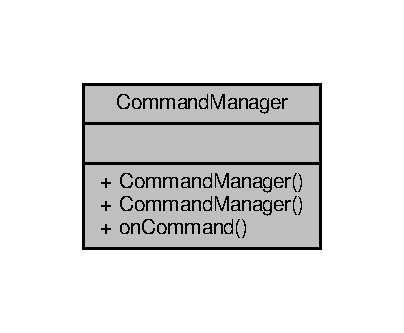
\includegraphics[width=246pt]{class_command_manager__coll__graph}
\end{center}
\end{figure}
\subsection*{Public Member Functions}
\begin{DoxyCompactItemize}
\item 
\hyperlink{class_command_manager_a8a13226bf933396a3f35dfb5bee3e813}{Command\-Manager} ()
\begin{DoxyCompactList}\small\item\em Init \hyperlink{class_command_manager}{Command\-Manager}. \end{DoxyCompactList}\item 
\hyperlink{class_command_manager_aeaffe7fa7dd8f1dd45b642120013a076}{Command\-Manager} (const \hyperlink{class_command_manager}{Command\-Manager} \&other)=delete
\item 
void \hyperlink{class_command_manager_abef8721bbe32e1ecb22f2f3d3b8c0601}{on\-Command} (\hyperlink{class_i_command_sender}{I\-Command\-Sender} $\ast$sender, const std\-::string \&cmd)
\item 
void \hyperlink{class_command_manager_a6782f9787d0e35ee3cc0eff69f764fa2}{execute\-Delayed\-Command\-In\-U\-I} ()
\end{DoxyCompactItemize}


\subsection{Detailed Description}
Send string-\/command through \hyperlink{class_command_manager}{Command\-Manager}. 

This is a very important class. Through this you can execute console-\/like text commands. 

\subsection{Constructor \& Destructor Documentation}
\hypertarget{class_command_manager_a8a13226bf933396a3f35dfb5bee3e813}{\index{Command\-Manager@{Command\-Manager}!Command\-Manager@{Command\-Manager}}
\index{Command\-Manager@{Command\-Manager}!CommandManager@{Command\-Manager}}
\subsubsection[{Command\-Manager}]{\setlength{\rightskip}{0pt plus 5cm}Command\-Manager\-::\-Command\-Manager (
\begin{DoxyParamCaption}
{}
\end{DoxyParamCaption}
)}}\label{class_command_manager_a8a13226bf933396a3f35dfb5bee3e813}


Init \hyperlink{class_command_manager}{Command\-Manager}. 

Adding all objects that extend \hyperlink{class_i_command}{I\-Command} to list (std\-::vector).

\begin{DoxyWarning}{Warning}
If you add an \hyperlink{class_i_command}{I\-Command}, you should add line here 
\end{DoxyWarning}
\hypertarget{class_command_manager_aeaffe7fa7dd8f1dd45b642120013a076}{\index{Command\-Manager@{Command\-Manager}!Command\-Manager@{Command\-Manager}}
\index{Command\-Manager@{Command\-Manager}!CommandManager@{Command\-Manager}}
\subsubsection[{Command\-Manager}]{\setlength{\rightskip}{0pt plus 5cm}Command\-Manager\-::\-Command\-Manager (
\begin{DoxyParamCaption}
\item[{const {\bf Command\-Manager} \&}]{other}
\end{DoxyParamCaption}
)\hspace{0.3cm}{\ttfamily [delete]}}}\label{class_command_manager_aeaffe7fa7dd8f1dd45b642120013a076}


\subsection{Member Function Documentation}
\hypertarget{class_command_manager_a6782f9787d0e35ee3cc0eff69f764fa2}{\index{Command\-Manager@{Command\-Manager}!execute\-Delayed\-Command\-In\-U\-I@{execute\-Delayed\-Command\-In\-U\-I}}
\index{execute\-Delayed\-Command\-In\-U\-I@{execute\-Delayed\-Command\-In\-U\-I}!CommandManager@{Command\-Manager}}
\subsubsection[{execute\-Delayed\-Command\-In\-U\-I}]{\setlength{\rightskip}{0pt plus 5cm}void Command\-Manager\-::execute\-Delayed\-Command\-In\-U\-I (
\begin{DoxyParamCaption}
{}
\end{DoxyParamCaption}
)}}\label{class_command_manager_a6782f9787d0e35ee3cc0eff69f764fa2}


Here is the call graph for this function\-:
\nopagebreak
\begin{figure}[H]
\begin{center}
\leavevmode
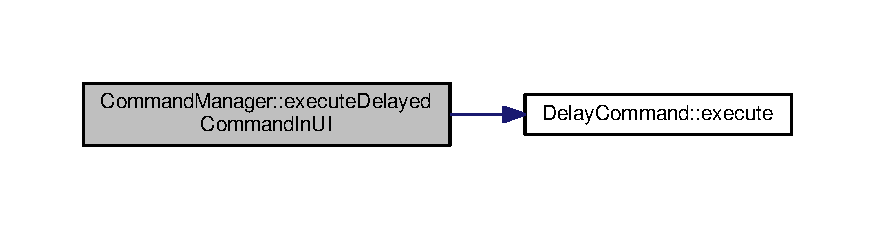
\includegraphics[width=350pt]{class_command_manager_a6782f9787d0e35ee3cc0eff69f764fa2_cgraph}
\end{center}
\end{figure}


\hypertarget{class_command_manager_abef8721bbe32e1ecb22f2f3d3b8c0601}{\index{Command\-Manager@{Command\-Manager}!on\-Command@{on\-Command}}
\index{on\-Command@{on\-Command}!CommandManager@{Command\-Manager}}
\subsubsection[{on\-Command}]{\setlength{\rightskip}{0pt plus 5cm}void Command\-Manager\-::on\-Command (
\begin{DoxyParamCaption}
\item[{{\bf I\-Command\-Sender} $\ast$}]{sender, }
\item[{const std\-::string \&}]{cmd}
\end{DoxyParamCaption}
)}}\label{class_command_manager_abef8721bbe32e1ecb22f2f3d3b8c0601}


Here is the call graph for this function\-:
\nopagebreak
\begin{figure}[H]
\begin{center}
\leavevmode
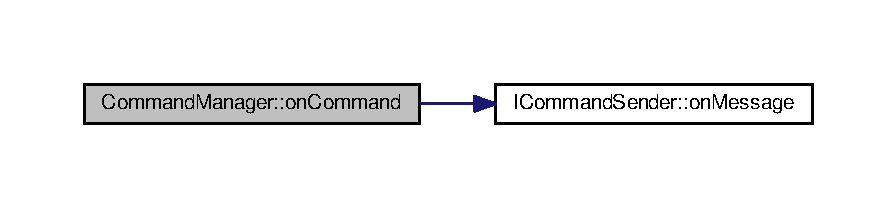
\includegraphics[width=350pt]{class_command_manager_abef8721bbe32e1ecb22f2f3d3b8c0601_cgraph}
\end{center}
\end{figure}




The documentation for this class was generated from the following files\-:\begin{DoxyCompactItemize}
\item 
/home/travis/build/bender-\/wardrobe/\-Recast/src/headers/commands/\hyperlink{_command_manager_8hpp}{Command\-Manager.\-hpp}\item 
/home/travis/build/bender-\/wardrobe/\-Recast/src/core/commands/\hyperlink{_command_manager_8cpp}{Command\-Manager.\-cpp}\end{DoxyCompactItemize}

\hypertarget{class_config}{\section{Config Class Reference}
\label{class_config}\index{Config@{Config}}
}


\hyperlink{class_config}{Config} class.  




{\ttfamily \#include $<$Config.\-hpp$>$}



Collaboration diagram for Config\-:
\nopagebreak
\begin{figure}[H]
\begin{center}
\leavevmode
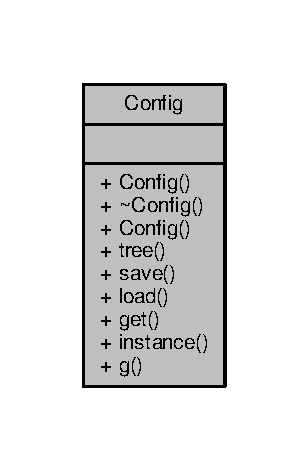
\includegraphics[width=148pt]{class_config__coll__graph}
\end{center}
\end{figure}
\subsection*{Public Member Functions}
\begin{DoxyCompactItemize}
\item 
\hyperlink{class_config_abc51a2c710c8666d27b53cc03597201d}{Config} (const std\-::string \&filename)
\item 
\hyperlink{class_config_a543dce59b66475c5108088ee4ce1cdfc}{$\sim$\-Config} ()
\item 
\hyperlink{class_config_aea1b7e862074892ee39a5583c342c482}{Config} (const \hyperlink{class_config}{Config} \&other)=delete
\item 
boost\-::property\-\_\-tree\-::ptree \& \hyperlink{class_config_a006701bd126aa5809b3a15e75c63bfb6}{tree} ()
\item 
void \hyperlink{class_config_ae7e68962f22a2c965a61702de1c637db}{save} ()
\item 
void \hyperlink{class_config_add4ebd0c89505c9b5368f03264555606}{load} ()
\item 
{\footnotesize template$<$class T $>$ }\\T \hyperlink{class_config_a1f8e429f853f20cac7cf128f2b71543e}{get} (const std\-::string \&key, T default\-Var)
\end{DoxyCompactItemize}
\subsection*{Static Public Member Functions}
\begin{DoxyCompactItemize}
\item 
static \hyperlink{class_config}{Config} $\ast$ \hyperlink{class_config_abf1d4539011ef83cac0fef2ac864a3a9}{instance} ()
\item 
{\footnotesize template$<$class T $>$ }\\static T \hyperlink{class_config_aaff6aaabead6b7486ec122f9dda807fd}{g} (const std\-::string \&key, T default\-Var)
\end{DoxyCompactItemize}


\subsection{Detailed Description}
\hyperlink{class_config}{Config} class. 

Using Boost ptree struct. \hyperlink{class_config}{Config} file hashing and buffering in memory. (You can't get an instance of \hyperlink{class_config}{Config} from constructor) Please call \hyperlink{class_config_abf1d4539011ef83cac0fef2ac864a3a9}{Config\-::instance} to get an instance of \hyperlink{class_config}{Config}. 

\subsection{Constructor \& Destructor Documentation}
\hypertarget{class_config_abc51a2c710c8666d27b53cc03597201d}{\index{Config@{Config}!Config@{Config}}
\index{Config@{Config}!Config@{Config}}
\subsubsection[{Config}]{\setlength{\rightskip}{0pt plus 5cm}Config\-::\-Config (
\begin{DoxyParamCaption}
\item[{const std\-::string \&}]{filename}
\end{DoxyParamCaption}
)}}\label{class_config_abc51a2c710c8666d27b53cc03597201d}
\hypertarget{class_config_a543dce59b66475c5108088ee4ce1cdfc}{\index{Config@{Config}!$\sim$\-Config@{$\sim$\-Config}}
\index{$\sim$\-Config@{$\sim$\-Config}!Config@{Config}}
\subsubsection[{$\sim$\-Config}]{\setlength{\rightskip}{0pt plus 5cm}Config\-::$\sim$\-Config (
\begin{DoxyParamCaption}
{}
\end{DoxyParamCaption}
)}}\label{class_config_a543dce59b66475c5108088ee4ce1cdfc}
\hypertarget{class_config_aea1b7e862074892ee39a5583c342c482}{\index{Config@{Config}!Config@{Config}}
\index{Config@{Config}!Config@{Config}}
\subsubsection[{Config}]{\setlength{\rightskip}{0pt plus 5cm}Config\-::\-Config (
\begin{DoxyParamCaption}
\item[{const {\bf Config} \&}]{other}
\end{DoxyParamCaption}
)\hspace{0.3cm}{\ttfamily [delete]}}}\label{class_config_aea1b7e862074892ee39a5583c342c482}


\subsection{Member Function Documentation}
\hypertarget{class_config_aaff6aaabead6b7486ec122f9dda807fd}{\index{Config@{Config}!g@{g}}
\index{g@{g}!Config@{Config}}
\subsubsection[{g}]{\setlength{\rightskip}{0pt plus 5cm}template$<$class T $>$ static T Config\-::g (
\begin{DoxyParamCaption}
\item[{const std\-::string \&}]{key, }
\item[{T}]{default\-Var}
\end{DoxyParamCaption}
)\hspace{0.3cm}{\ttfamily [inline]}, {\ttfamily [static]}}}\label{class_config_aaff6aaabead6b7486ec122f9dda807fd}


Here is the call graph for this function\-:
\nopagebreak
\begin{figure}[H]
\begin{center}
\leavevmode
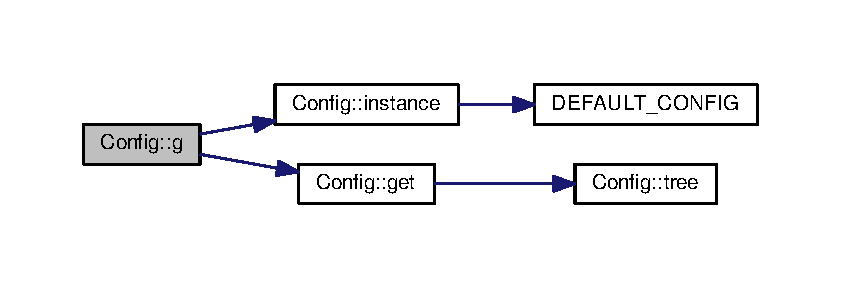
\includegraphics[width=350pt]{class_config_aaff6aaabead6b7486ec122f9dda807fd_cgraph}
\end{center}
\end{figure}




Here is the caller graph for this function\-:
\nopagebreak
\begin{figure}[H]
\begin{center}
\leavevmode
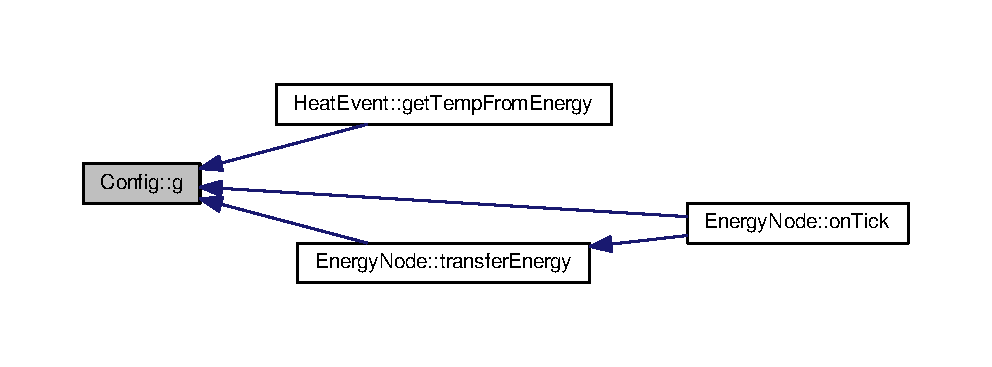
\includegraphics[width=350pt]{class_config_aaff6aaabead6b7486ec122f9dda807fd_icgraph}
\end{center}
\end{figure}


\hypertarget{class_config_a1f8e429f853f20cac7cf128f2b71543e}{\index{Config@{Config}!get@{get}}
\index{get@{get}!Config@{Config}}
\subsubsection[{get}]{\setlength{\rightskip}{0pt plus 5cm}template$<$class T $>$ T Config\-::get (
\begin{DoxyParamCaption}
\item[{const std\-::string \&}]{key, }
\item[{T}]{default\-Var}
\end{DoxyParamCaption}
)\hspace{0.3cm}{\ttfamily [inline]}}}\label{class_config_a1f8e429f853f20cac7cf128f2b71543e}
This method create param if not exist


\begin{DoxyTemplParams}{Template Parameters}
{\em T} & class of config var \\
\hline
\end{DoxyTemplParams}

\begin{DoxyParams}{Parameters}
{\em key} & string with path like 'general.\-server.\-port' \\
\hline
{\em default\-Var} & var used when config var is empty \\
\hline
\end{DoxyParams}
\begin{DoxyReturn}{Returns}
defult\-Var returned if config var is empty 
\end{DoxyReturn}


Here is the call graph for this function\-:
\nopagebreak
\begin{figure}[H]
\begin{center}
\leavevmode
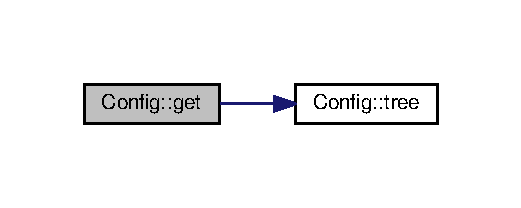
\includegraphics[width=250pt]{class_config_a1f8e429f853f20cac7cf128f2b71543e_cgraph}
\end{center}
\end{figure}




Here is the caller graph for this function\-:
\nopagebreak
\begin{figure}[H]
\begin{center}
\leavevmode
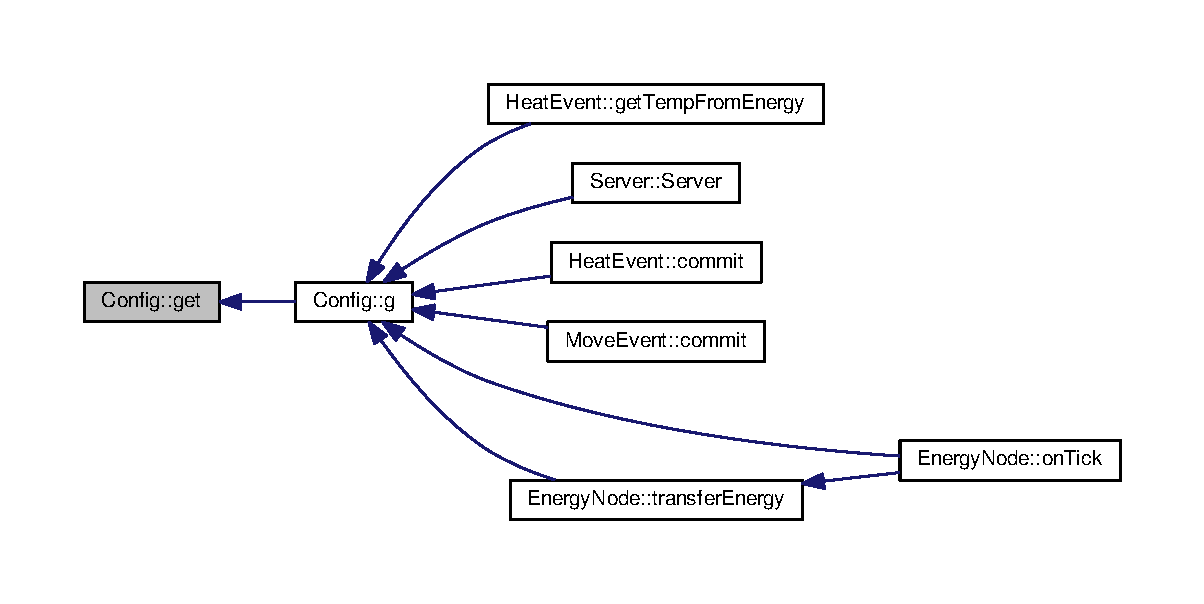
\includegraphics[width=350pt]{class_config_a1f8e429f853f20cac7cf128f2b71543e_icgraph}
\end{center}
\end{figure}


\hypertarget{class_config_abf1d4539011ef83cac0fef2ac864a3a9}{\index{Config@{Config}!instance@{instance}}
\index{instance@{instance}!Config@{Config}}
\subsubsection[{instance}]{\setlength{\rightskip}{0pt plus 5cm}{\bf Config} $\ast$ Config\-::instance (
\begin{DoxyParamCaption}
{}
\end{DoxyParamCaption}
)\hspace{0.3cm}{\ttfamily [static]}}}\label{class_config_abf1d4539011ef83cac0fef2ac864a3a9}


Here is the call graph for this function\-:
\nopagebreak
\begin{figure}[H]
\begin{center}
\leavevmode
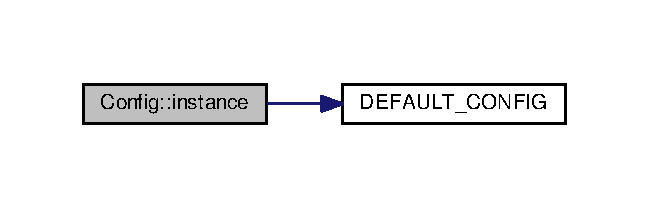
\includegraphics[width=312pt]{class_config_abf1d4539011ef83cac0fef2ac864a3a9_cgraph}
\end{center}
\end{figure}




Here is the caller graph for this function\-:
\nopagebreak
\begin{figure}[H]
\begin{center}
\leavevmode
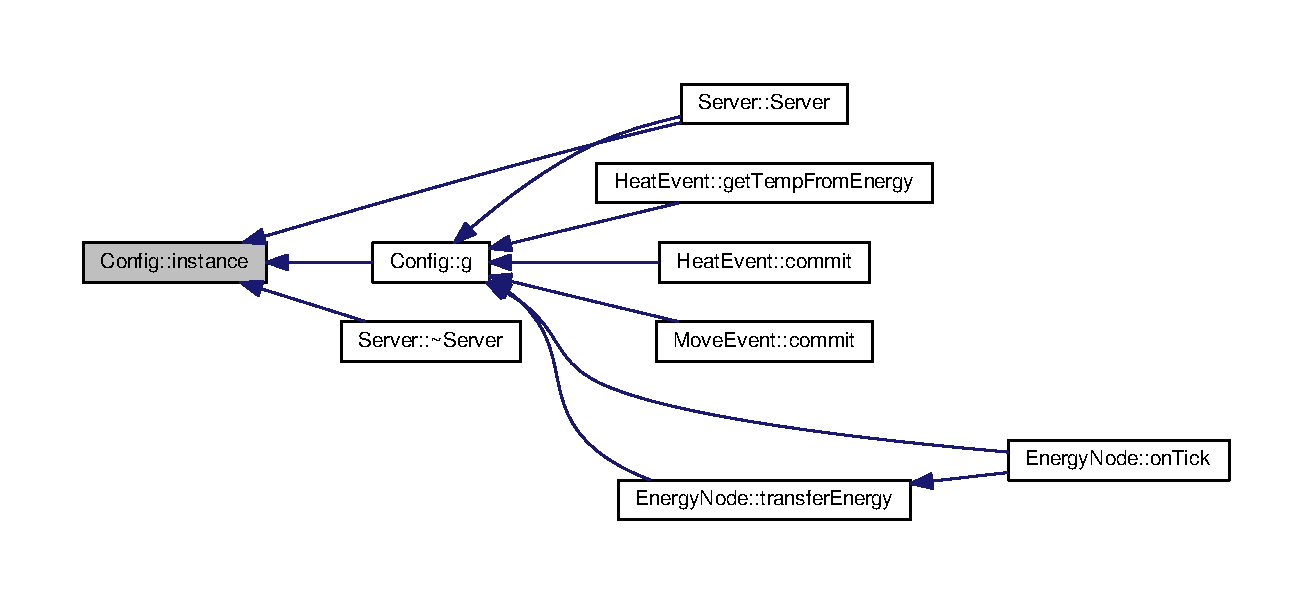
\includegraphics[width=350pt]{class_config_abf1d4539011ef83cac0fef2ac864a3a9_icgraph}
\end{center}
\end{figure}


\hypertarget{class_config_add4ebd0c89505c9b5368f03264555606}{\index{Config@{Config}!load@{load}}
\index{load@{load}!Config@{Config}}
\subsubsection[{load}]{\setlength{\rightskip}{0pt plus 5cm}void Config\-::load (
\begin{DoxyParamCaption}
{}
\end{DoxyParamCaption}
)}}\label{class_config_add4ebd0c89505c9b5368f03264555606}
\hypertarget{class_config_ae7e68962f22a2c965a61702de1c637db}{\index{Config@{Config}!save@{save}}
\index{save@{save}!Config@{Config}}
\subsubsection[{save}]{\setlength{\rightskip}{0pt plus 5cm}void Config\-::save (
\begin{DoxyParamCaption}
{}
\end{DoxyParamCaption}
)}}\label{class_config_ae7e68962f22a2c965a61702de1c637db}


Here is the call graph for this function\-:
\nopagebreak
\begin{figure}[H]
\begin{center}
\leavevmode
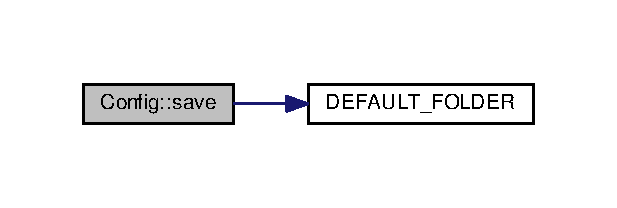
\includegraphics[width=296pt]{class_config_ae7e68962f22a2c965a61702de1c637db_cgraph}
\end{center}
\end{figure}


\hypertarget{class_config_a006701bd126aa5809b3a15e75c63bfb6}{\index{Config@{Config}!tree@{tree}}
\index{tree@{tree}!Config@{Config}}
\subsubsection[{tree}]{\setlength{\rightskip}{0pt plus 5cm}ptree \& Config\-::tree (
\begin{DoxyParamCaption}
{}
\end{DoxyParamCaption}
)}}\label{class_config_a006701bd126aa5809b3a15e75c63bfb6}


Here is the caller graph for this function\-:
\nopagebreak
\begin{figure}[H]
\begin{center}
\leavevmode
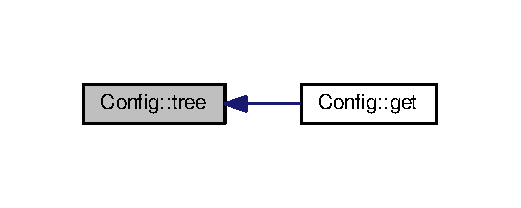
\includegraphics[width=350pt]{class_config_a006701bd126aa5809b3a15e75c63bfb6_icgraph}
\end{center}
\end{figure}




The documentation for this class was generated from the following files\-:\begin{DoxyCompactItemize}
\item 
/home/travis/build/bender-\/wardrobe/\-Recast/src/headers/io/configs/\hyperlink{_config_8hpp}{Config.\-hpp}\item 
/home/travis/build/bender-\/wardrobe/\-Recast/src/core/io/configs/\hyperlink{_config_8cpp}{Config.\-cpp}\end{DoxyCompactItemize}

\hypertarget{class_i_command}{\section{I\-Command Class Reference}
\label{class_i_command}\index{I\-Command@{I\-Command}}
}


Superclass for Command object.  




{\ttfamily \#include $<$I\-Command.\-hpp$>$}



Inheritance diagram for I\-Command\-:
\nopagebreak
\begin{figure}[H]
\begin{center}
\leavevmode
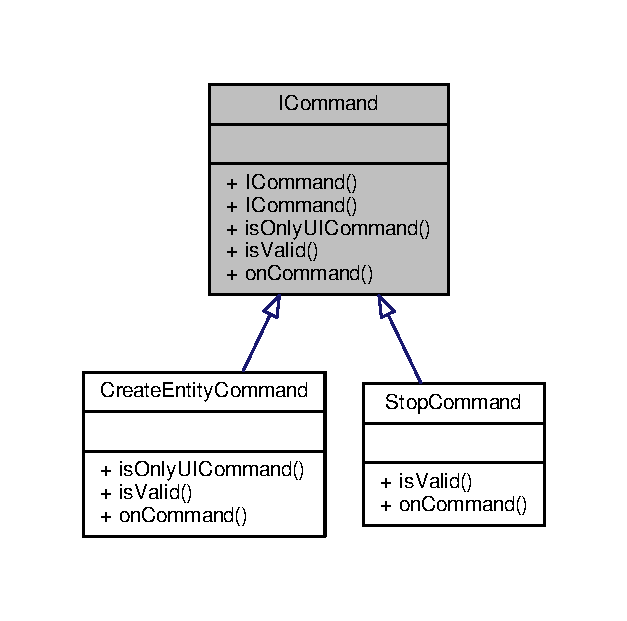
\includegraphics[width=301pt]{class_i_command__inherit__graph}
\end{center}
\end{figure}


Collaboration diagram for I\-Command\-:
\nopagebreak
\begin{figure}[H]
\begin{center}
\leavevmode
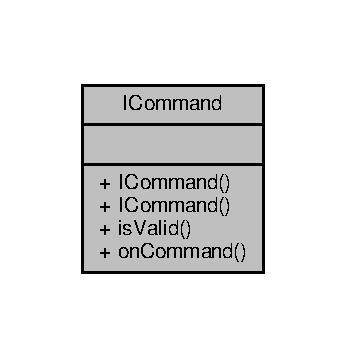
\includegraphics[width=194pt]{class_i_command__coll__graph}
\end{center}
\end{figure}
\subsection*{Public Member Functions}
\begin{DoxyCompactItemize}
\item 
\hyperlink{class_i_command_acf142bc073aaf829663ba395bacd34cc}{I\-Command} ()
\item 
\hyperlink{class_i_command_a1a3e297aea5c94d785060e49801860dc}{I\-Command} (const \hyperlink{class_i_command}{I\-Command} \&other)
\item 
virtual bool \hyperlink{class_i_command_ac2bd771dcd2fda5a951869bdc4928b48}{is\-Only\-U\-I\-Command} ()
\item 
virtual bool \hyperlink{class_i_command_acb0beea12bd5ec963884dc35d4d48014}{is\-Valid} (const std\-::string \&cmd, const std\-::vector$<$ std\-::string $>$ \&args) const =0
\item 
virtual void \hyperlink{class_i_command_a55f931bb7304e2bc591ba2edd717e86c}{on\-Command} (\hyperlink{class_i_command_sender}{I\-Command\-Sender} \&sender, const std\-::string \&cmd, const std\-::vector$<$ std\-::string $>$ \&args)=0
\end{DoxyCompactItemize}


\subsection{Detailed Description}
Superclass for Command object. 

If you want to create new command you should extend \hyperlink{class_i_command}{I\-Command} class and register that in \hyperlink{class_command_manager}{Command\-Manager} constructor

\begin{DoxyWarning}{Warning}
Don't forget to register your Command in Command\-Manager!!! 
\end{DoxyWarning}


\subsection{Constructor \& Destructor Documentation}
\hypertarget{class_i_command_acf142bc073aaf829663ba395bacd34cc}{\index{I\-Command@{I\-Command}!I\-Command@{I\-Command}}
\index{I\-Command@{I\-Command}!ICommand@{I\-Command}}
\subsubsection[{I\-Command}]{\setlength{\rightskip}{0pt plus 5cm}I\-Command\-::\-I\-Command (
\begin{DoxyParamCaption}
{}
\end{DoxyParamCaption}
)\hspace{0.3cm}{\ttfamily [inline]}}}\label{class_i_command_acf142bc073aaf829663ba395bacd34cc}
\hypertarget{class_i_command_a1a3e297aea5c94d785060e49801860dc}{\index{I\-Command@{I\-Command}!I\-Command@{I\-Command}}
\index{I\-Command@{I\-Command}!ICommand@{I\-Command}}
\subsubsection[{I\-Command}]{\setlength{\rightskip}{0pt plus 5cm}I\-Command\-::\-I\-Command (
\begin{DoxyParamCaption}
\item[{const {\bf I\-Command} \&}]{other}
\end{DoxyParamCaption}
)\hspace{0.3cm}{\ttfamily [inline]}}}\label{class_i_command_a1a3e297aea5c94d785060e49801860dc}


\subsection{Member Function Documentation}
\hypertarget{class_i_command_ac2bd771dcd2fda5a951869bdc4928b48}{\index{I\-Command@{I\-Command}!is\-Only\-U\-I\-Command@{is\-Only\-U\-I\-Command}}
\index{is\-Only\-U\-I\-Command@{is\-Only\-U\-I\-Command}!ICommand@{I\-Command}}
\subsubsection[{is\-Only\-U\-I\-Command}]{\setlength{\rightskip}{0pt plus 5cm}virtual bool I\-Command\-::is\-Only\-U\-I\-Command (
\begin{DoxyParamCaption}
{}
\end{DoxyParamCaption}
)\hspace{0.3cm}{\ttfamily [inline]}, {\ttfamily [virtual]}}}\label{class_i_command_ac2bd771dcd2fda5a951869bdc4928b48}


Reimplemented in \hyperlink{class_create_entity_command_a8cb21ea7a4b172a26e2a3e62586a1c4a}{Create\-Entity\-Command}.

\hypertarget{class_i_command_acb0beea12bd5ec963884dc35d4d48014}{\index{I\-Command@{I\-Command}!is\-Valid@{is\-Valid}}
\index{is\-Valid@{is\-Valid}!ICommand@{I\-Command}}
\subsubsection[{is\-Valid}]{\setlength{\rightskip}{0pt plus 5cm}virtual bool I\-Command\-::is\-Valid (
\begin{DoxyParamCaption}
\item[{const std\-::string \&}]{cmd, }
\item[{const std\-::vector$<$ std\-::string $>$ \&}]{args}
\end{DoxyParamCaption}
) const\hspace{0.3cm}{\ttfamily [pure virtual]}}}\label{class_i_command_acb0beea12bd5ec963884dc35d4d48014}


Implemented in \hyperlink{class_create_entity_command_abeba611ac32b8d438736a383cf5f041f}{Create\-Entity\-Command}, and \hyperlink{class_stop_command_a0f9a9fd9bb238524e1be3ea25b9bbb79}{Stop\-Command}.

\hypertarget{class_i_command_a55f931bb7304e2bc591ba2edd717e86c}{\index{I\-Command@{I\-Command}!on\-Command@{on\-Command}}
\index{on\-Command@{on\-Command}!ICommand@{I\-Command}}
\subsubsection[{on\-Command}]{\setlength{\rightskip}{0pt plus 5cm}virtual void I\-Command\-::on\-Command (
\begin{DoxyParamCaption}
\item[{{\bf I\-Command\-Sender} \&}]{sender, }
\item[{const std\-::string \&}]{cmd, }
\item[{const std\-::vector$<$ std\-::string $>$ \&}]{args}
\end{DoxyParamCaption}
)\hspace{0.3cm}{\ttfamily [pure virtual]}}}\label{class_i_command_a55f931bb7304e2bc591ba2edd717e86c}


Implemented in \hyperlink{class_create_entity_command_aacb06adba7b70b5a5225c72bf943bab2}{Create\-Entity\-Command}, and \hyperlink{class_stop_command_a5f1df22a117e1f9afd65f0c55dcfc983}{Stop\-Command}.



The documentation for this class was generated from the following file\-:\begin{DoxyCompactItemize}
\item 
/home/travis/build/glitchless/\-Recast/src/headers/commands/\hyperlink{_i_command_8hpp}{I\-Command.\-hpp}\end{DoxyCompactItemize}

\hypertarget{class_i_command_sender}{\section{I\-Command\-Sender Class Reference}
\label{class_i_command_sender}\index{I\-Command\-Sender@{I\-Command\-Sender}}
}


{\ttfamily \#include $<$I\-Command\-Sender.\-hpp$>$}



Inheritance diagram for I\-Command\-Sender\-:
\nopagebreak
\begin{figure}[H]
\begin{center}
\leavevmode
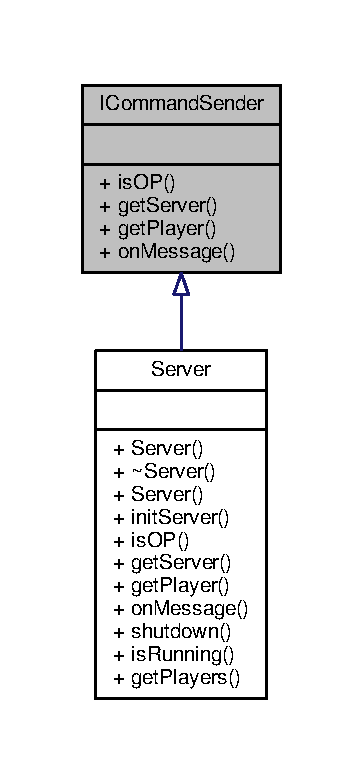
\includegraphics[width=204pt]{class_i_command_sender__inherit__graph}
\end{center}
\end{figure}


Collaboration diagram for I\-Command\-Sender\-:
\nopagebreak
\begin{figure}[H]
\begin{center}
\leavevmode
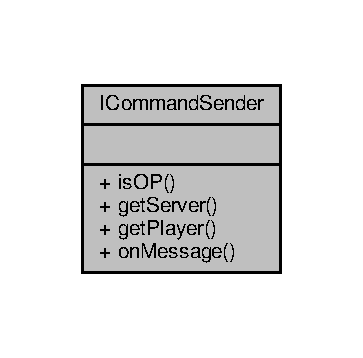
\includegraphics[width=174pt]{class_i_command_sender__coll__graph}
\end{center}
\end{figure}
\subsection*{Public Member Functions}
\begin{DoxyCompactItemize}
\item 
virtual bool \hyperlink{class_i_command_sender_afe930466c485c8d9a67f624dc1dcac5e}{is\-O\-P} () const =0
\item 
virtual \hyperlink{class_server}{Server} $\ast$ \hyperlink{class_i_command_sender_afe665fdd44daefad719049b540fc14b9}{get\-Server} ()=0
\item 
virtual \hyperlink{struct_player}{Player} $\ast$ \hyperlink{class_i_command_sender_abe8ec89d12e5de40cec1062da47f336c}{get\-Player} ()=0
\item 
virtual void \hyperlink{class_i_command_sender_a613b27b190c7fb5123597939c0896080}{on\-Message} (const std\-::string \&msg)=0
\end{DoxyCompactItemize}


\subsection{Member Function Documentation}
\hypertarget{class_i_command_sender_abe8ec89d12e5de40cec1062da47f336c}{\index{I\-Command\-Sender@{I\-Command\-Sender}!get\-Player@{get\-Player}}
\index{get\-Player@{get\-Player}!ICommandSender@{I\-Command\-Sender}}
\subsubsection[{get\-Player}]{\setlength{\rightskip}{0pt plus 5cm}virtual {\bf Player}$\ast$ I\-Command\-Sender\-::get\-Player (
\begin{DoxyParamCaption}
{}
\end{DoxyParamCaption}
)\hspace{0.3cm}{\ttfamily [pure virtual]}}}\label{class_i_command_sender_abe8ec89d12e5de40cec1062da47f336c}


Implemented in \hyperlink{class_server_a35be365123751e27d6c52ad3962b9b1e}{Server}.

\hypertarget{class_i_command_sender_afe665fdd44daefad719049b540fc14b9}{\index{I\-Command\-Sender@{I\-Command\-Sender}!get\-Server@{get\-Server}}
\index{get\-Server@{get\-Server}!ICommandSender@{I\-Command\-Sender}}
\subsubsection[{get\-Server}]{\setlength{\rightskip}{0pt plus 5cm}virtual {\bf Server}$\ast$ I\-Command\-Sender\-::get\-Server (
\begin{DoxyParamCaption}
{}
\end{DoxyParamCaption}
)\hspace{0.3cm}{\ttfamily [pure virtual]}}}\label{class_i_command_sender_afe665fdd44daefad719049b540fc14b9}


Implemented in \hyperlink{class_server_a8af940772beedcc0b1243adf3f5aec0c}{Server}.



Here is the caller graph for this function\-:
\nopagebreak
\begin{figure}[H]
\begin{center}
\leavevmode
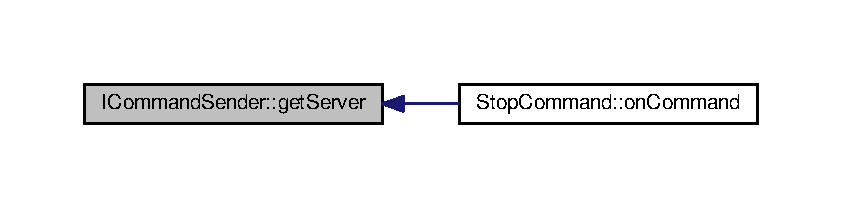
\includegraphics[width=350pt]{class_i_command_sender_afe665fdd44daefad719049b540fc14b9_icgraph}
\end{center}
\end{figure}


\hypertarget{class_i_command_sender_afe930466c485c8d9a67f624dc1dcac5e}{\index{I\-Command\-Sender@{I\-Command\-Sender}!is\-O\-P@{is\-O\-P}}
\index{is\-O\-P@{is\-O\-P}!ICommandSender@{I\-Command\-Sender}}
\subsubsection[{is\-O\-P}]{\setlength{\rightskip}{0pt plus 5cm}virtual bool I\-Command\-Sender\-::is\-O\-P (
\begin{DoxyParamCaption}
{}
\end{DoxyParamCaption}
) const\hspace{0.3cm}{\ttfamily [pure virtual]}}}\label{class_i_command_sender_afe930466c485c8d9a67f624dc1dcac5e}


Implemented in \hyperlink{class_server_a7b6439f1e85af364215c544d675ea972}{Server}.



Here is the caller graph for this function\-:
\nopagebreak
\begin{figure}[H]
\begin{center}
\leavevmode
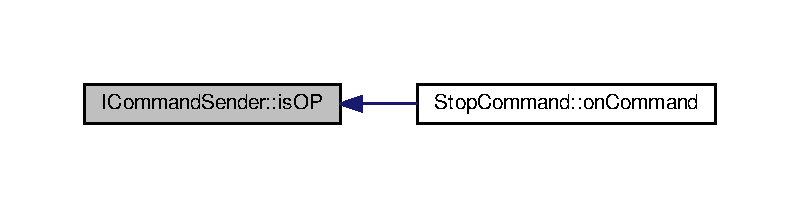
\includegraphics[width=350pt]{class_i_command_sender_afe930466c485c8d9a67f624dc1dcac5e_icgraph}
\end{center}
\end{figure}


\hypertarget{class_i_command_sender_a613b27b190c7fb5123597939c0896080}{\index{I\-Command\-Sender@{I\-Command\-Sender}!on\-Message@{on\-Message}}
\index{on\-Message@{on\-Message}!ICommandSender@{I\-Command\-Sender}}
\subsubsection[{on\-Message}]{\setlength{\rightskip}{0pt plus 5cm}virtual void I\-Command\-Sender\-::on\-Message (
\begin{DoxyParamCaption}
\item[{const std\-::string \&}]{msg}
\end{DoxyParamCaption}
)\hspace{0.3cm}{\ttfamily [pure virtual]}}}\label{class_i_command_sender_a613b27b190c7fb5123597939c0896080}


Implemented in \hyperlink{class_server_a37a56fedea3137e9b8080ee0e86e8278}{Server}.



Here is the caller graph for this function\-:
\nopagebreak
\begin{figure}[H]
\begin{center}
\leavevmode
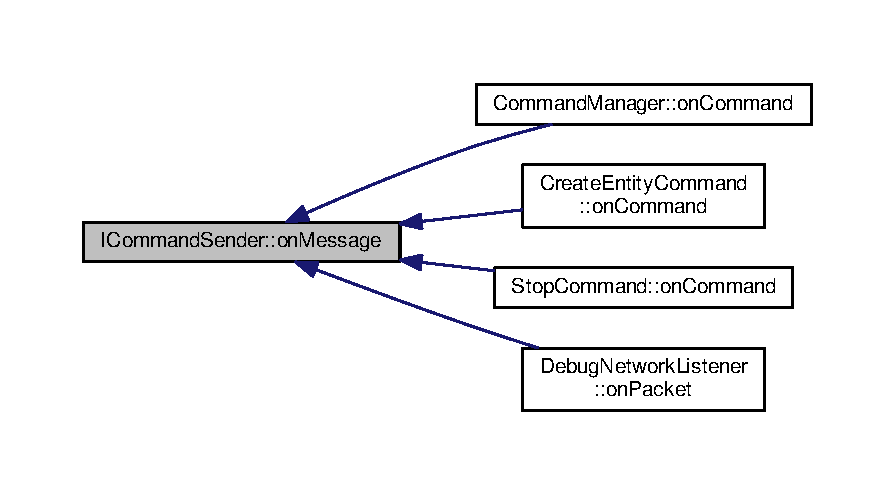
\includegraphics[width=350pt]{class_i_command_sender_a613b27b190c7fb5123597939c0896080_icgraph}
\end{center}
\end{figure}




The documentation for this class was generated from the following file\-:\begin{DoxyCompactItemize}
\item 
/home/travis/build/bender-\/wardrobe/\-Recast/src/headers/commands/\hyperlink{_i_command_sender_8hpp}{I\-Command\-Sender.\-hpp}\end{DoxyCompactItemize}

\hypertarget{class_player}{\section{Player Class Reference}
\label{class_player}\index{Player@{Player}}
}


\hyperlink{class_player}{Player} class.  




{\ttfamily \#include $<$Player.\-h$>$}



\subsection{Detailed Description}
\hyperlink{class_player}{Player} class. 

Lol. Aka Context for \hyperlink{class_player}{Player} only. 

The documentation for this class was generated from the following file\-:\begin{DoxyCompactItemize}
\item 
/home/travis/build/bender-\/wardrobe/\-Recast/src/headers/models/\hyperlink{_player_8h}{Player.\-h}\end{DoxyCompactItemize}

\hypertarget{struct_point}{\section{Point Struct Reference}
\label{struct_point}\index{Point@{Point}}
}


Just point.  




{\ttfamily \#include $<$Point.\-h$>$}



Collaboration diagram for Point\-:
\nopagebreak
\begin{figure}[H]
\begin{center}
\leavevmode
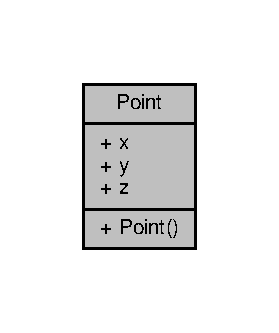
\includegraphics[width=134pt]{struct_point__coll__graph}
\end{center}
\end{figure}
\subsection*{Public Member Functions}
\begin{DoxyCompactItemize}
\item 
\hyperlink{struct_point_a4d43f5247afe8c85c6da1aa39dbcc738}{Point} (double \hyperlink{struct_point_ab99c56589bc8ad5fa5071387110a5bc7}{x}, double \hyperlink{struct_point_afa38be143ae800e6ad69ce8ed4df62d8}{y}, double \hyperlink{struct_point_a05ba3b1dfcb19430582ae953cbbfbded}{z})
\end{DoxyCompactItemize}
\subsection*{Public Attributes}
\begin{DoxyCompactItemize}
\item 
double \hyperlink{struct_point_ab99c56589bc8ad5fa5071387110a5bc7}{x}
\item 
double \hyperlink{struct_point_afa38be143ae800e6ad69ce8ed4df62d8}{y}
\item 
double \hyperlink{struct_point_a05ba3b1dfcb19430582ae953cbbfbded}{z}
\end{DoxyCompactItemize}


\subsection{Detailed Description}
Just point. 

It't \hyperlink{struct_point}{Point}. James \hyperlink{struct_point}{Point}. 

\subsection{Constructor \& Destructor Documentation}
\hypertarget{struct_point_a4d43f5247afe8c85c6da1aa39dbcc738}{\index{Point@{Point}!Point@{Point}}
\index{Point@{Point}!Point@{Point}}
\subsubsection[{Point}]{\setlength{\rightskip}{0pt plus 5cm}Point\-::\-Point (
\begin{DoxyParamCaption}
\item[{double}]{x, }
\item[{double}]{y, }
\item[{double}]{z}
\end{DoxyParamCaption}
)\hspace{0.3cm}{\ttfamily [inline]}}}\label{struct_point_a4d43f5247afe8c85c6da1aa39dbcc738}


\subsection{Member Data Documentation}
\hypertarget{struct_point_ab99c56589bc8ad5fa5071387110a5bc7}{\index{Point@{Point}!x@{x}}
\index{x@{x}!Point@{Point}}
\subsubsection[{x}]{\setlength{\rightskip}{0pt plus 5cm}double Point\-::x}}\label{struct_point_ab99c56589bc8ad5fa5071387110a5bc7}
\hypertarget{struct_point_afa38be143ae800e6ad69ce8ed4df62d8}{\index{Point@{Point}!y@{y}}
\index{y@{y}!Point@{Point}}
\subsubsection[{y}]{\setlength{\rightskip}{0pt plus 5cm}double Point\-::y}}\label{struct_point_afa38be143ae800e6ad69ce8ed4df62d8}
\hypertarget{struct_point_a05ba3b1dfcb19430582ae953cbbfbded}{\index{Point@{Point}!z@{z}}
\index{z@{z}!Point@{Point}}
\subsubsection[{z}]{\setlength{\rightskip}{0pt plus 5cm}double Point\-::z}}\label{struct_point_a05ba3b1dfcb19430582ae953cbbfbded}


The documentation for this struct was generated from the following file\-:\begin{DoxyCompactItemize}
\item 
/home/travis/build/bender-\/wardrobe/\-Recast/src/headers/models/\hyperlink{_point_8h}{Point.\-h}\end{DoxyCompactItemize}

\hypertarget{class_server}{\section{Server Class Reference}
\label{class_server}\index{Server@{Server}}
}


Main class in Recast \hyperlink{class_server}{Server}.  




{\ttfamily \#include $<$Server.\-h$>$}



Inheritance diagram for Server\-:
\nopagebreak
\begin{figure}[H]
\begin{center}
\leavevmode
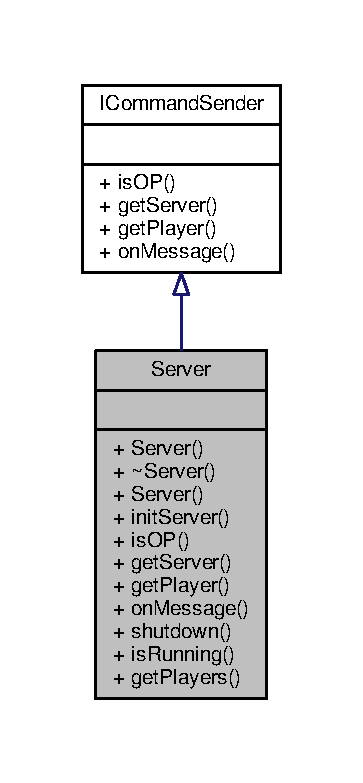
\includegraphics[width=174pt]{class_server__inherit__graph}
\end{center}
\end{figure}


Collaboration diagram for Server\-:
\nopagebreak
\begin{figure}[H]
\begin{center}
\leavevmode
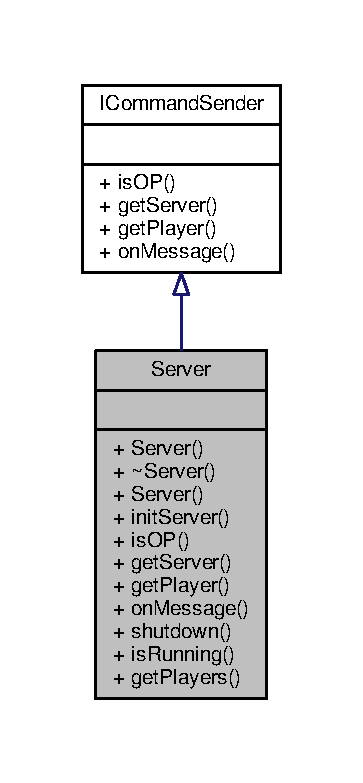
\includegraphics[width=174pt]{class_server__coll__graph}
\end{center}
\end{figure}
\subsection*{Public Member Functions}
\begin{DoxyCompactItemize}
\item 
\hypertarget{class_server_aca4a9834f8bf136619d3c4cdb1db4e1e}{{\bfseries Server} (const \hyperlink{class_server}{Server} \&other)=delete}\label{class_server_aca4a9834f8bf136619d3c4cdb1db4e1e}

\item 
\hypertarget{class_server_a7bc5c00fa3ae1ddfae71274ee7d025ea}{void {\bfseries init\-Server} ()}\label{class_server_a7bc5c00fa3ae1ddfae71274ee7d025ea}

\item 
\hypertarget{class_server_a7b6439f1e85af364215c544d675ea972}{bool {\bfseries is\-O\-P} () const }\label{class_server_a7b6439f1e85af364215c544d675ea972}

\item 
\hypertarget{class_server_a8af940772beedcc0b1243adf3f5aec0c}{\hyperlink{class_server}{Server} $\ast$ {\bfseries get\-Server} ()}\label{class_server_a8af940772beedcc0b1243adf3f5aec0c}

\item 
\hypertarget{class_server_a35be365123751e27d6c52ad3962b9b1e}{\hyperlink{class_player}{Player} $\ast$ {\bfseries get\-Player} ()}\label{class_server_a35be365123751e27d6c52ad3962b9b1e}

\item 
\hypertarget{class_server_a37a56fedea3137e9b8080ee0e86e8278}{void {\bfseries on\-Message} (const std\-::string \&msg)}\label{class_server_a37a56fedea3137e9b8080ee0e86e8278}

\item 
\hypertarget{class_server_a58c74bafaaf20b24e9243c7cf5fdfd16}{bool {\bfseries shutdown} ()}\label{class_server_a58c74bafaaf20b24e9243c7cf5fdfd16}

\item 
\hypertarget{class_server_ab8c22a0d6809e9aa84bebce478ba7bc5}{bool {\bfseries is\-Running} () const }\label{class_server_ab8c22a0d6809e9aa84bebce478ba7bc5}

\end{DoxyCompactItemize}


\subsection{Detailed Description}
Main class in Recast \hyperlink{class_server}{Server}. 

The documentation for this class was generated from the following files\-:\begin{DoxyCompactItemize}
\item 
/home/travis/build/bender-\/wardrobe/\-Recast/src/headers/\hyperlink{_server_8h}{Server.\-h}\item 
/home/travis/build/bender-\/wardrobe/\-Recast/src/\hyperlink{_server_8cpp}{Server.\-cpp}\end{DoxyCompactItemize}

\hypertarget{class_stop_command}{\section{Stop\-Command Class Reference}
\label{class_stop_command}\index{Stop\-Command@{Stop\-Command}}
}


{\ttfamily \#include $<$Stop\-Command.\-hpp$>$}



Inheritance diagram for Stop\-Command\-:
\nopagebreak
\begin{figure}[H]
\begin{center}
\leavevmode
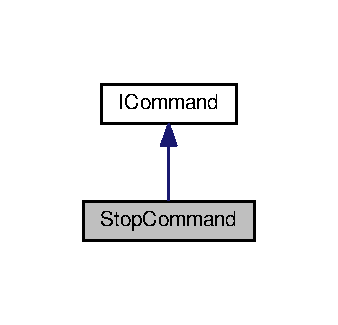
\includegraphics[width=166pt]{class_stop_command__inherit__graph}
\end{center}
\end{figure}


Collaboration diagram for Stop\-Command\-:
\nopagebreak
\begin{figure}[H]
\begin{center}
\leavevmode
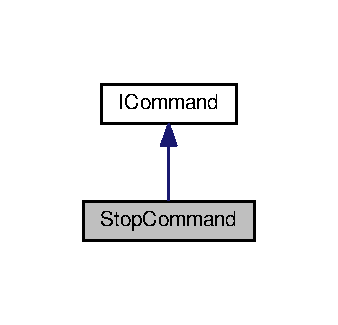
\includegraphics[width=166pt]{class_stop_command__coll__graph}
\end{center}
\end{figure}
\subsection*{Public Member Functions}
\begin{DoxyCompactItemize}
\item 
bool \hyperlink{class_stop_command_a0f9a9fd9bb238524e1be3ea25b9bbb79}{is\-Valid} (const std\-::string \&cmd, const std\-::vector$<$ std\-::string $>$ \&args) const 
\item 
void \hyperlink{class_stop_command_a5f1df22a117e1f9afd65f0c55dcfc983}{on\-Command} (\hyperlink{class_i_command_sender}{I\-Command\-Sender} \&sender, const std\-::string \&cmd, const std\-::vector$<$ std\-::string $>$ \&args)
\end{DoxyCompactItemize}


\subsection{Member Function Documentation}
\hypertarget{class_stop_command_a0f9a9fd9bb238524e1be3ea25b9bbb79}{\index{Stop\-Command@{Stop\-Command}!is\-Valid@{is\-Valid}}
\index{is\-Valid@{is\-Valid}!StopCommand@{Stop\-Command}}
\subsubsection[{is\-Valid}]{\setlength{\rightskip}{0pt plus 5cm}bool Stop\-Command\-::is\-Valid (
\begin{DoxyParamCaption}
\item[{const std\-::string \&}]{cmd, }
\item[{const std\-::vector$<$ std\-::string $>$ \&}]{args}
\end{DoxyParamCaption}
) const\hspace{0.3cm}{\ttfamily [virtual]}}}\label{class_stop_command_a0f9a9fd9bb238524e1be3ea25b9bbb79}


Implements \hyperlink{class_i_command_acb0beea12bd5ec963884dc35d4d48014}{I\-Command}.

\hypertarget{class_stop_command_a5f1df22a117e1f9afd65f0c55dcfc983}{\index{Stop\-Command@{Stop\-Command}!on\-Command@{on\-Command}}
\index{on\-Command@{on\-Command}!StopCommand@{Stop\-Command}}
\subsubsection[{on\-Command}]{\setlength{\rightskip}{0pt plus 5cm}void Stop\-Command\-::on\-Command (
\begin{DoxyParamCaption}
\item[{{\bf I\-Command\-Sender} \&}]{sender, }
\item[{const std\-::string \&}]{cmd, }
\item[{const std\-::vector$<$ std\-::string $>$ \&}]{args}
\end{DoxyParamCaption}
)\hspace{0.3cm}{\ttfamily [virtual]}}}\label{class_stop_command_a5f1df22a117e1f9afd65f0c55dcfc983}


Implements \hyperlink{class_i_command_a55f931bb7304e2bc591ba2edd717e86c}{I\-Command}.



Here is the call graph for this function\-:
\nopagebreak
\begin{figure}[H]
\begin{center}
\leavevmode
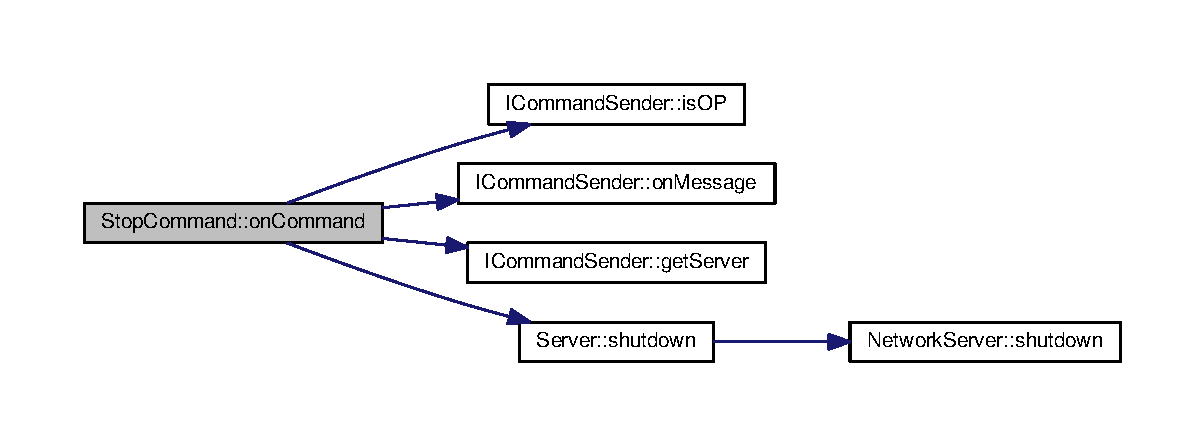
\includegraphics[width=350pt]{class_stop_command_a5f1df22a117e1f9afd65f0c55dcfc983_cgraph}
\end{center}
\end{figure}




The documentation for this class was generated from the following files\-:\begin{DoxyCompactItemize}
\item 
/home/travis/build/bender-\/wardrobe/\-Recast/src/headers/commands/\hyperlink{_stop_command_8hpp}{Stop\-Command.\-hpp}\item 
/home/travis/build/bender-\/wardrobe/\-Recast/src/core/commands/\hyperlink{_stop_command_8cpp}{Stop\-Command.\-cpp}\end{DoxyCompactItemize}

\chapter{File Documentation}
\hypertarget{_command_manager_8cpp}{\section{/home/travis/build/glitchless/\-Recast/src/core/commands/\-Command\-Manager.cpp File Reference}
\label{_command_manager_8cpp}\index{/home/travis/build/glitchless/\-Recast/src/core/commands/\-Command\-Manager.\-cpp@{/home/travis/build/glitchless/\-Recast/src/core/commands/\-Command\-Manager.\-cpp}}
}


\hyperlink{class_command_manager}{Command\-Manager} description.  


{\ttfamily \#include $<$sstream$>$}\\*
{\ttfamily \#include $<$iterator$>$}\\*
{\ttfamily \#include $<$memory$>$}\\*
{\ttfamily \#include $<$vector$>$}\\*
{\ttfamily \#include $<$commands/\-Create\-Entity\-Command.\-h$>$}\\*
{\ttfamily \#include \char`\"{}commands/\-Command\-Manager.\-hpp\char`\"{}}\\*
{\ttfamily \#include \char`\"{}commands/\-Stop\-Command.\-hpp\char`\"{}}\\*
Include dependency graph for Command\-Manager.\-cpp\-:
\nopagebreak
\begin{figure}[H]
\begin{center}
\leavevmode
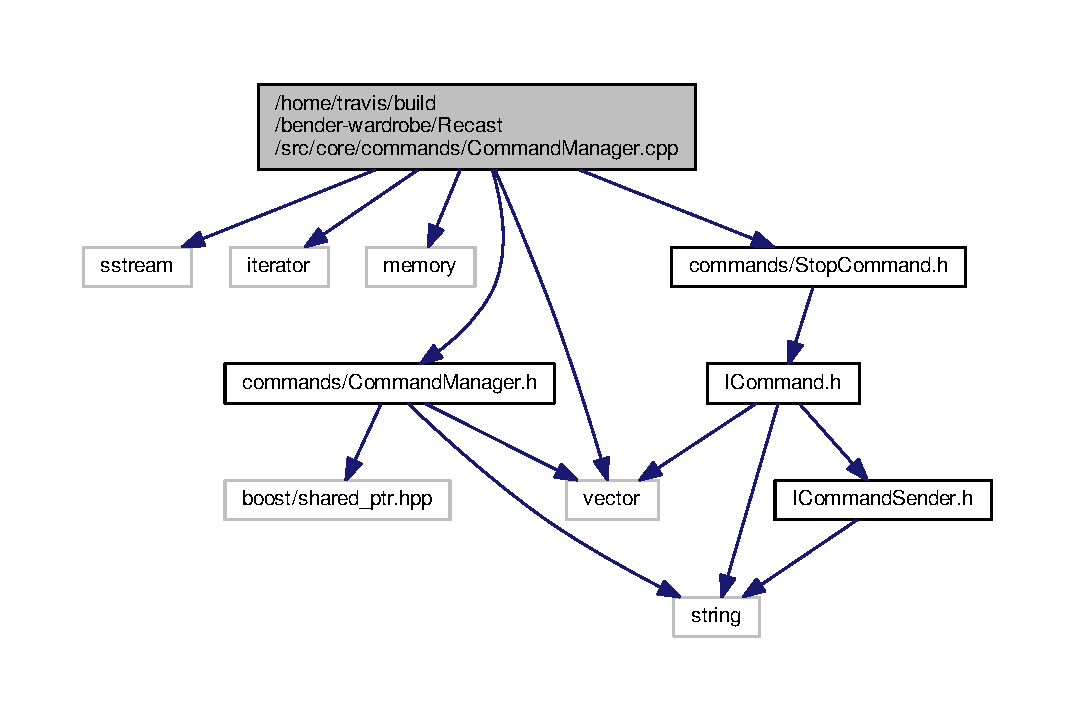
\includegraphics[width=350pt]{_command_manager_8cpp__incl}
\end{center}
\end{figure}


\subsection{Detailed Description}
\hyperlink{class_command_manager}{Command\-Manager} description. \begin{DoxyAuthor}{Author}
Lion\-Z\-X\-Y  Recast-\/server 
\end{DoxyAuthor}
\begin{DoxyDate}{Date}
08.\-06.\-17
\end{DoxyDate}
\hyperlink{class_command_manager}{Command\-Manager} description 
\hypertarget{_i_command_8cpp}{\section{/home/travis/build/bender-\/wardrobe/\-Recast/src/core/commands/\-I\-Command.cpp File Reference}
\label{_i_command_8cpp}\index{/home/travis/build/bender-\/wardrobe/\-Recast/src/core/commands/\-I\-Command.\-cpp@{/home/travis/build/bender-\/wardrobe/\-Recast/src/core/commands/\-I\-Command.\-cpp}}
}


\hyperlink{class_i_command}{I\-Command} some method.  


{\ttfamily \#include \char`\"{}commands/\-I\-Command.\-h\char`\"{}}\\*
Include dependency graph for I\-Command.\-cpp\-:
\nopagebreak
\begin{figure}[H]
\begin{center}
\leavevmode
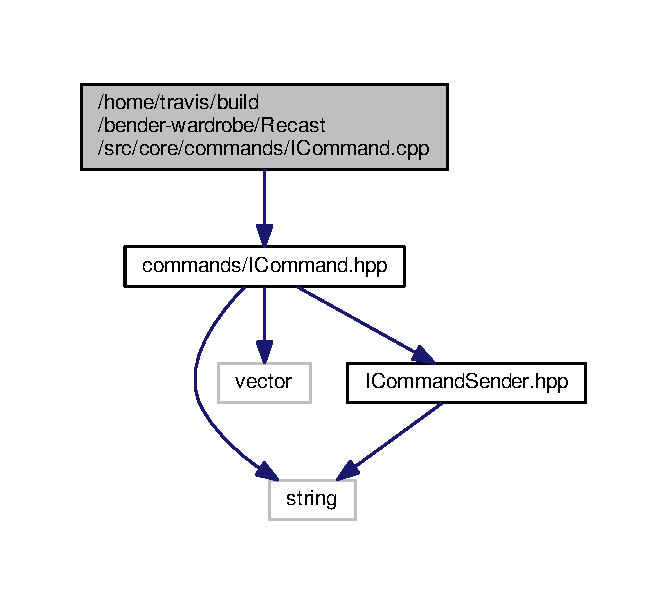
\includegraphics[width=311pt]{_i_command_8cpp__incl}
\end{center}
\end{figure}


\subsection{Detailed Description}
\hyperlink{class_i_command}{I\-Command} some method. \begin{DoxyAuthor}{Author}
Lion\-Z\-X\-Y  Recast-\/server 
\end{DoxyAuthor}
\begin{DoxyDate}{Date}
08.\-06.\-17
\end{DoxyDate}
Now do nothing \-:3 
\hypertarget{_i_command_sender_8cpp}{\section{/home/travis/build/glitchless/\-Recast/src/core/commands/\-I\-Command\-Sender.cpp File Reference}
\label{_i_command_sender_8cpp}\index{/home/travis/build/glitchless/\-Recast/src/core/commands/\-I\-Command\-Sender.\-cpp@{/home/travis/build/glitchless/\-Recast/src/core/commands/\-I\-Command\-Sender.\-cpp}}
}


\hyperlink{class_i_command_sender}{I\-Command\-Sender} file for other method.  


{\ttfamily \#include \char`\"{}commands/\-I\-Command\-Sender.\-hpp\char`\"{}}\\*
Include dependency graph for I\-Command\-Sender.\-cpp\-:
\nopagebreak
\begin{figure}[H]
\begin{center}
\leavevmode
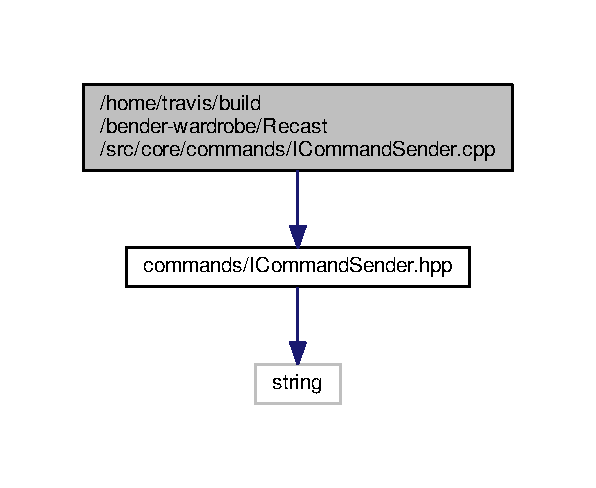
\includegraphics[width=270pt]{_i_command_sender_8cpp__incl}
\end{center}
\end{figure}


\subsection{Detailed Description}
\hyperlink{class_i_command_sender}{I\-Command\-Sender} file for other method. \begin{DoxyAuthor}{Author}
Lion\-Z\-X\-Y  Recast-\/server 
\end{DoxyAuthor}
\begin{DoxyDate}{Date}
08.\-06.\-17
\end{DoxyDate}
Now do nothing \-:3 
\hypertarget{_config_8cpp}{\section{/home/travis/build/bender-\/wardrobe/\-Recast/src/core/configs/\-Config.cpp File Reference}
\label{_config_8cpp}\index{/home/travis/build/bender-\/wardrobe/\-Recast/src/core/configs/\-Config.\-cpp@{/home/travis/build/bender-\/wardrobe/\-Recast/src/core/configs/\-Config.\-cpp}}
}


\hyperlink{class_config}{Config} description.  


{\ttfamily \#include $<$boost/property\-\_\-tree/json\-\_\-parser.\-hpp$>$}\\*
{\ttfamily \#include $<$boost/filesystem.\-hpp$>$}\\*
{\ttfamily \#include $<$boost/log/trivial.\-hpp$>$}\\*
{\ttfamily \#include \char`\"{}configs/\-Config.\-h\char`\"{}}\\*
Include dependency graph for Config.\-cpp\-:
\nopagebreak
\begin{figure}[H]
\begin{center}
\leavevmode
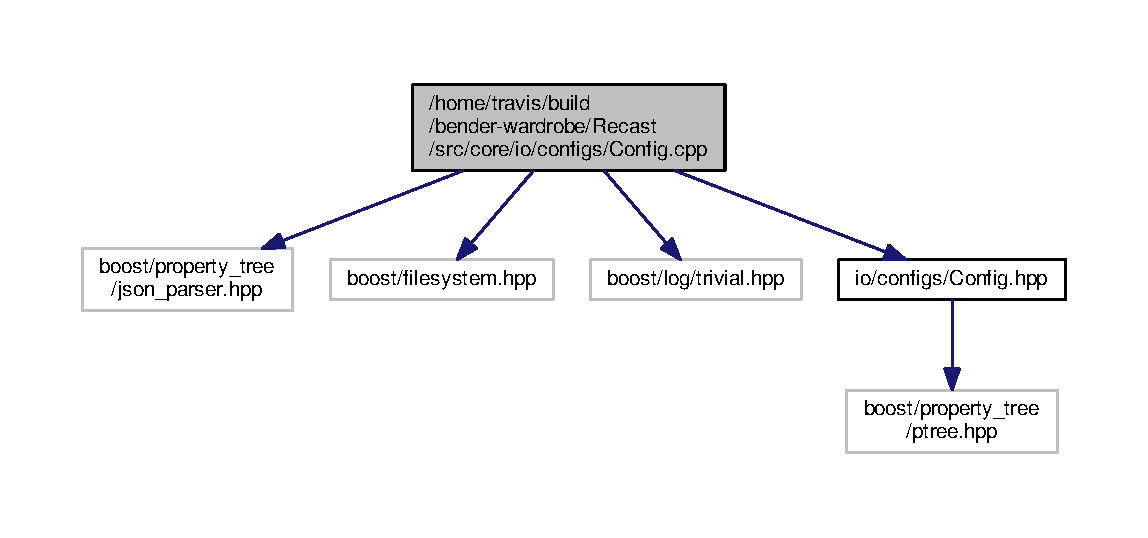
\includegraphics[width=350pt]{_config_8cpp__incl}
\end{center}
\end{figure}
\subsection*{Functions}
\begin{DoxyCompactItemize}
\item 
\hypertarget{_config_8cpp_a26d7091acfa5c363d348bbe5043b5c39}{const string {\bfseries D\-E\-F\-A\-U\-L\-T\-\_\-\-F\-O\-L\-D\-E\-R} (\char`\"{}./config/\char`\"{})}\label{_config_8cpp_a26d7091acfa5c363d348bbe5043b5c39}

\item 
\hypertarget{_config_8cpp_ab330b966aa1026a8014370d5732fae26}{const string {\bfseries D\-E\-F\-A\-U\-L\-T\-\_\-\-C\-O\-N\-F\-I\-G} (\char`\"{}general.\-json\char`\"{})}\label{_config_8cpp_ab330b966aa1026a8014370d5732fae26}

\end{DoxyCompactItemize}
\subsection*{Variables}
\begin{DoxyCompactItemize}
\item 
\hypertarget{_config_8cpp_af80efdbf1a16321cb0fbb1e695a114bf}{const int {\bfseries C\-O\-N\-F\-I\-G\-\_\-\-V\-E\-R\-S\-I\-O\-N} = 1}\label{_config_8cpp_af80efdbf1a16321cb0fbb1e695a114bf}

\item 
\hypertarget{_config_8cpp_a7609d9a81c0d8e5f318598fc94afdaf5}{const int {\bfseries N\-O\-T\-H\-I\-N\-G} = -\/1}\label{_config_8cpp_a7609d9a81c0d8e5f318598fc94afdaf5}

\end{DoxyCompactItemize}


\subsection{Detailed Description}
\hyperlink{class_config}{Config} description. \begin{DoxyAuthor}{Author}
Lion\-Z\-X\-Y  Recast 
\end{DoxyAuthor}
\begin{DoxyDate}{Date}
08.\-06.\-17
\end{DoxyDate}
Save I\-N\-S\-T\-A\-N\-C\-E config and get if you need this. 
\hypertarget{_command_manager_8h}{\section{/home/travis/build/bender-\/wardrobe/\-Recast/src/headers/commands/\-Command\-Manager.h File Reference}
\label{_command_manager_8h}\index{/home/travis/build/bender-\/wardrobe/\-Recast/src/headers/commands/\-Command\-Manager.\-h@{/home/travis/build/bender-\/wardrobe/\-Recast/src/headers/commands/\-Command\-Manager.\-h}}
}


\hyperlink{class_command_manager}{Command\-Manager} file.  


{\ttfamily \#include $<$vector$>$}\\*
{\ttfamily \#include $<$string$>$}\\*
{\ttfamily \#include $<$boost/shared\-\_\-ptr.\-hpp$>$}\\*
Include dependency graph for Command\-Manager.\-h\-:
\nopagebreak
\begin{figure}[H]
\begin{center}
\leavevmode
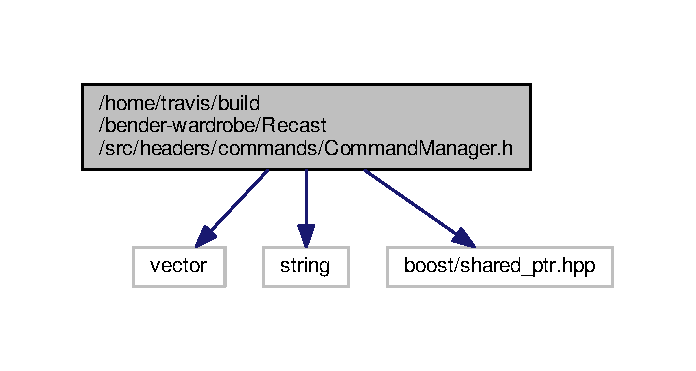
\includegraphics[width=334pt]{_command_manager_8h__incl}
\end{center}
\end{figure}
This graph shows which files directly or indirectly include this file\-:
\nopagebreak
\begin{figure}[H]
\begin{center}
\leavevmode
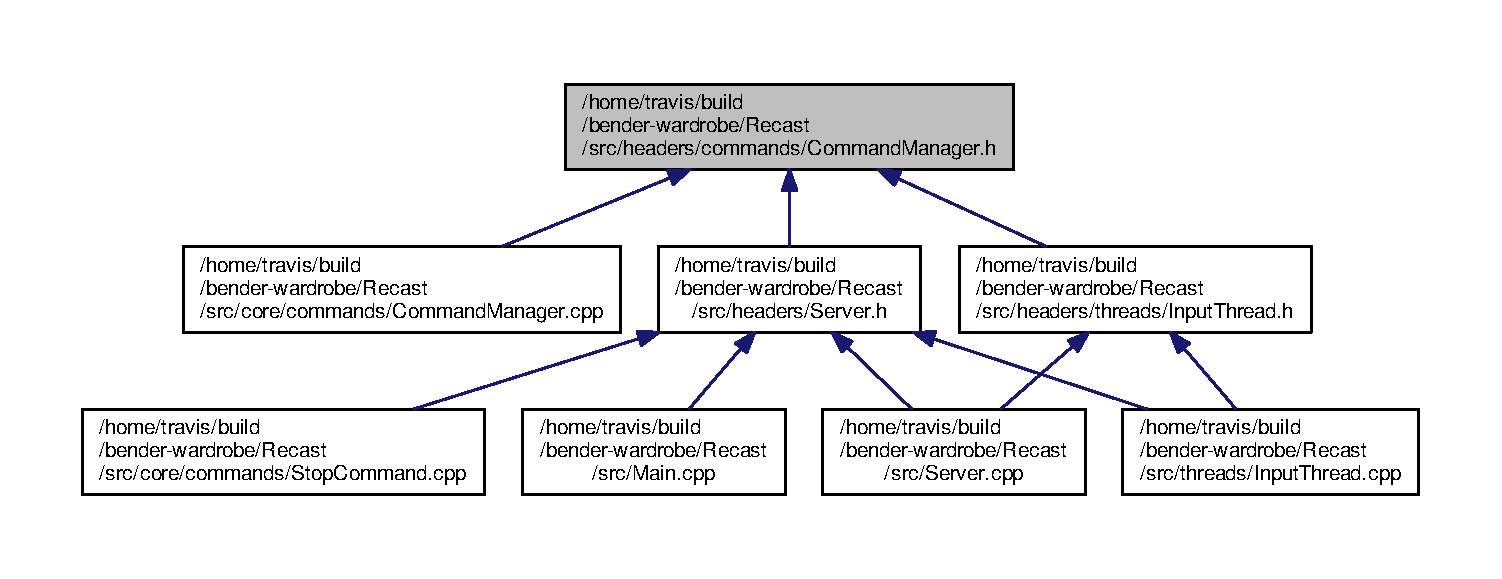
\includegraphics[width=350pt]{_command_manager_8h__dep__incl}
\end{center}
\end{figure}
\subsection*{Classes}
\begin{DoxyCompactItemize}
\item 
class \hyperlink{class_command_manager}{Command\-Manager}
\begin{DoxyCompactList}\small\item\em Send string-\/command through \hyperlink{class_command_manager}{Command\-Manager}. \end{DoxyCompactList}\end{DoxyCompactItemize}


\subsection{Detailed Description}
\hyperlink{class_command_manager}{Command\-Manager} file. \begin{DoxyAuthor}{Author}
Lion\-Z\-X\-Y  Recast-\/server 
\end{DoxyAuthor}
\begin{DoxyDate}{Date}
08.\-06.\-17
\end{DoxyDate}
Command manager file 
\hypertarget{_i_command_8h}{\section{/home/travis/build/bender-\/wardrobe/\-Recast/src/headers/commands/\-I\-Command.h File Reference}
\label{_i_command_8h}\index{/home/travis/build/bender-\/wardrobe/\-Recast/src/headers/commands/\-I\-Command.\-h@{/home/travis/build/bender-\/wardrobe/\-Recast/src/headers/commands/\-I\-Command.\-h}}
}


Command file.  


{\ttfamily \#include $<$string$>$}\\*
{\ttfamily \#include $<$vector$>$}\\*
{\ttfamily \#include \char`\"{}I\-Command\-Sender.\-h\char`\"{}}\\*
Include dependency graph for I\-Command.\-h\-:
\nopagebreak
\begin{figure}[H]
\begin{center}
\leavevmode
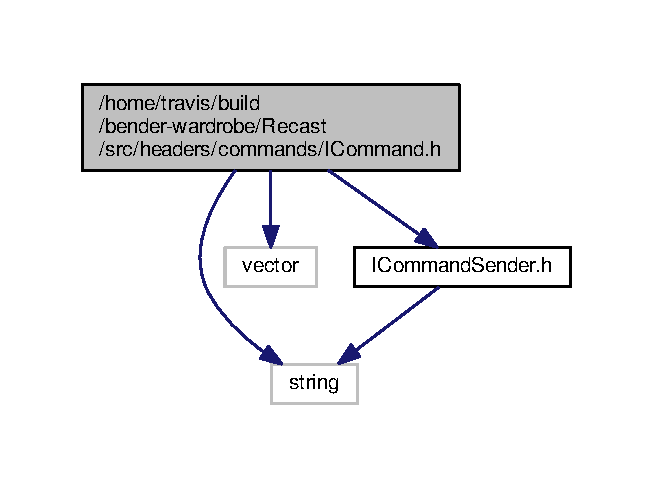
\includegraphics[width=314pt]{_i_command_8h__incl}
\end{center}
\end{figure}
This graph shows which files directly or indirectly include this file\-:
\nopagebreak
\begin{figure}[H]
\begin{center}
\leavevmode
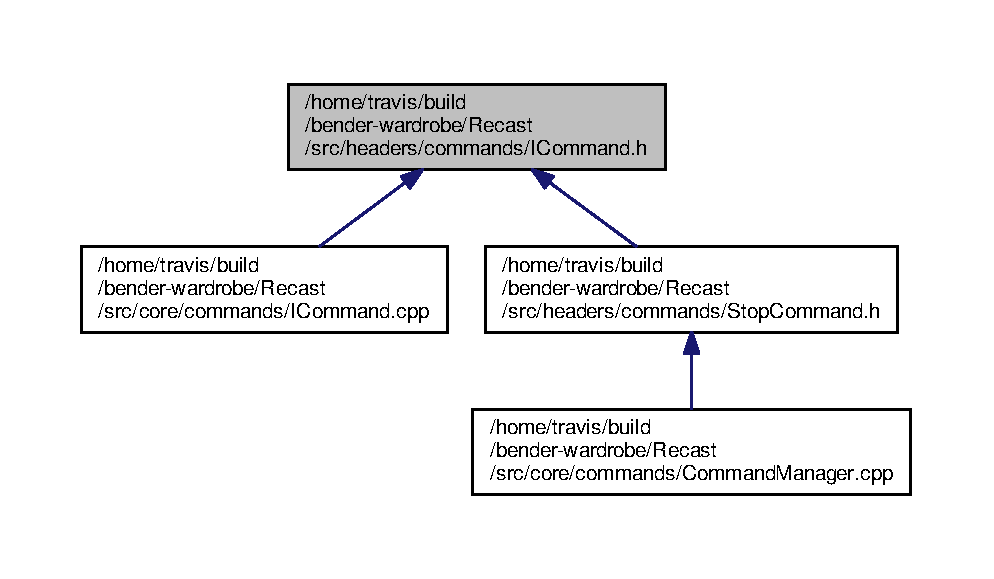
\includegraphics[width=350pt]{_i_command_8h__dep__incl}
\end{center}
\end{figure}
\subsection*{Classes}
\begin{DoxyCompactItemize}
\item 
class \hyperlink{class_i_command}{I\-Command}
\begin{DoxyCompactList}\small\item\em Superclass for Command object. \end{DoxyCompactList}\end{DoxyCompactItemize}


\subsection{Detailed Description}
Command file. \begin{DoxyAuthor}{Author}
Lion\-Z\-X\-Y  Recast-\/server 
\end{DoxyAuthor}
\begin{DoxyDate}{Date}
08.\-06.\-17
\end{DoxyDate}
Describe I\-Command\-File 
\hypertarget{_config_8h}{\section{/home/travis/build/bender-\/wardrobe/\-Recast/src/headers/configs/\-Config.h File Reference}
\label{_config_8h}\index{/home/travis/build/bender-\/wardrobe/\-Recast/src/headers/configs/\-Config.\-h@{/home/travis/build/bender-\/wardrobe/\-Recast/src/headers/configs/\-Config.\-h}}
}


\hyperlink{class_config}{Config} file.  


{\ttfamily \#include $<$boost/property\-\_\-tree/ptree.\-hpp$>$}\\*
Include dependency graph for Config.\-h\-:
\nopagebreak
\begin{figure}[H]
\begin{center}
\leavevmode
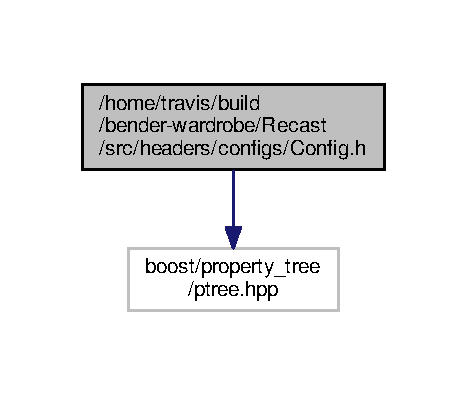
\includegraphics[width=224pt]{_config_8h__incl}
\end{center}
\end{figure}
This graph shows which files directly or indirectly include this file\-:
\nopagebreak
\begin{figure}[H]
\begin{center}
\leavevmode
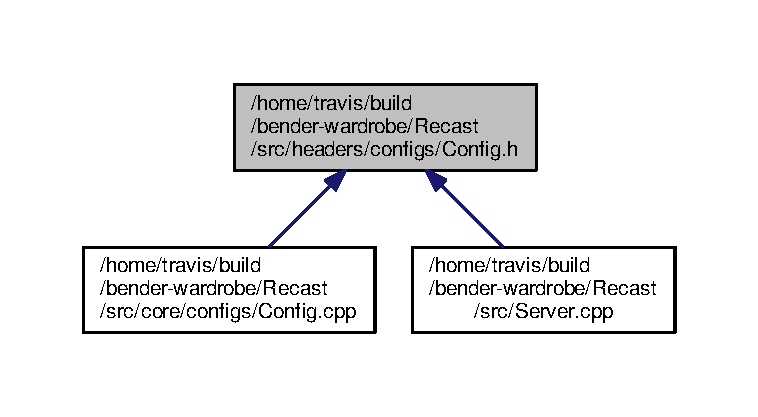
\includegraphics[width=350pt]{_config_8h__dep__incl}
\end{center}
\end{figure}
\subsection*{Classes}
\begin{DoxyCompactItemize}
\item 
class \hyperlink{class_config}{Config}
\begin{DoxyCompactList}\small\item\em \hyperlink{class_config}{Config} class. \end{DoxyCompactList}\end{DoxyCompactItemize}


\subsection{Detailed Description}
\hyperlink{class_config}{Config} file. \begin{DoxyAuthor}{Author}
Lion\-Z\-X\-Y  Recast 
\end{DoxyAuthor}
\begin{DoxyDate}{Date}
08.\-06.\-17
\end{DoxyDate}
\hyperlink{class_config}{Config} file. 
\hypertarget{_player_8h}{\section{/home/travis/build/bender-\/wardrobe/\-Recast/src/headers/models/\-Player.h File Reference}
\label{_player_8h}\index{/home/travis/build/bender-\/wardrobe/\-Recast/src/headers/models/\-Player.\-h@{/home/travis/build/bender-\/wardrobe/\-Recast/src/headers/models/\-Player.\-h}}
}


\hyperlink{struct_player}{Player} file.  


{\ttfamily \#include \char`\"{}Point.\-h\char`\"{}}\\*
Include dependency graph for Player.\-h\-:
\nopagebreak
\begin{figure}[H]
\begin{center}
\leavevmode
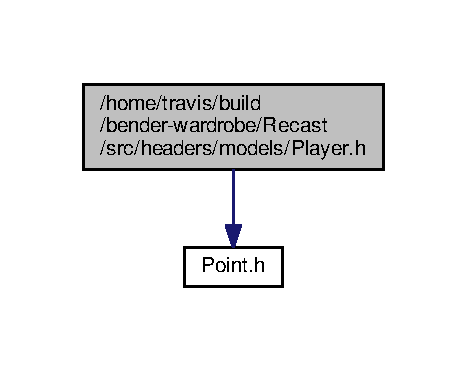
\includegraphics[width=224pt]{_player_8h__incl}
\end{center}
\end{figure}
This graph shows which files directly or indirectly include this file\-:
\nopagebreak
\begin{figure}[H]
\begin{center}
\leavevmode
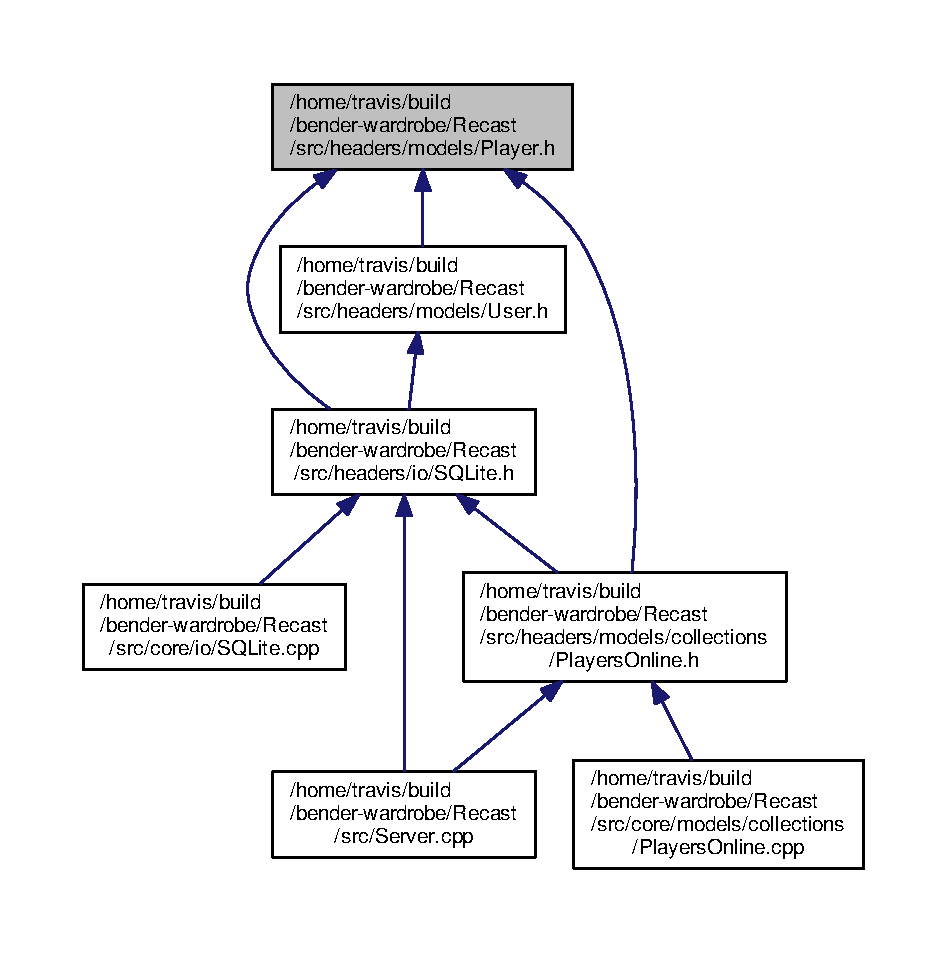
\includegraphics[width=350pt]{_player_8h__dep__incl}
\end{center}
\end{figure}
\subsection*{Classes}
\begin{DoxyCompactItemize}
\item 
struct \hyperlink{struct_player}{Player}
\begin{DoxyCompactList}\small\item\em \hyperlink{struct_player}{Player} class. X\-P, Life points and other. \end{DoxyCompactList}\end{DoxyCompactItemize}


\subsection{Detailed Description}
\hyperlink{struct_player}{Player} file. \begin{DoxyAuthor}{Author}
Lion\-Z\-X\-Y  Recast-\/server 
\end{DoxyAuthor}
\begin{DoxyDate}{Date}
08.\-06.\-17
\end{DoxyDate}
\hyperlink{struct_player}{Player} file 
\hypertarget{_server_8h}{\section{/home/travis/build/bender-\/wardrobe/\-Recast/src/headers/\-Server.h File Reference}
\label{_server_8h}\index{/home/travis/build/bender-\/wardrobe/\-Recast/src/headers/\-Server.\-h@{/home/travis/build/bender-\/wardrobe/\-Recast/src/headers/\-Server.\-h}}
}


\hyperlink{class_server}{Server} file.  


{\ttfamily \#include $<$string$>$}\\*
{\ttfamily \#include $<$thread$>$}\\*
{\ttfamily \#include \char`\"{}commands/\-I\-Command\-Sender.\-h\char`\"{}}\\*
{\ttfamily \#include \char`\"{}commands/\-Command\-Manager.\-h\char`\"{}}\\*
{\ttfamily \#include \char`\"{}temperature-\/world/interfaces/\-I\-Updater.\-hpp\char`\"{}}\\*
{\ttfamily \#include \char`\"{}temperature-\/world/interfaces/\-I\-Temperature\-World\-Chunkable\-Observable.\-hpp\char`\"{}}\\*
{\ttfamily \#include \char`\"{}temperature-\/world/interfaces/\-I\-Temperature\-World\-Chunkable\-Generatable.\-hpp\char`\"{}}\\*
{\ttfamily \#include \char`\"{}temperature-\/world/interfaces/\-I\-Temperature\-World\-Chunkable\-Mutable.\-hpp\char`\"{}}\\*
{\ttfamily \#include \char`\"{}temperature-\/world/interfaces/\-I\-Temperature\-World\-Chunkable.\-hpp\char`\"{}}\\*
{\ttfamily \#include \char`\"{}temperature-\/world/interfaces/\-I\-Temperature\-World.\-hpp\char`\"{}}\\*
Include dependency graph for Server.\-h\-:
\nopagebreak
\begin{figure}[H]
\begin{center}
\leavevmode
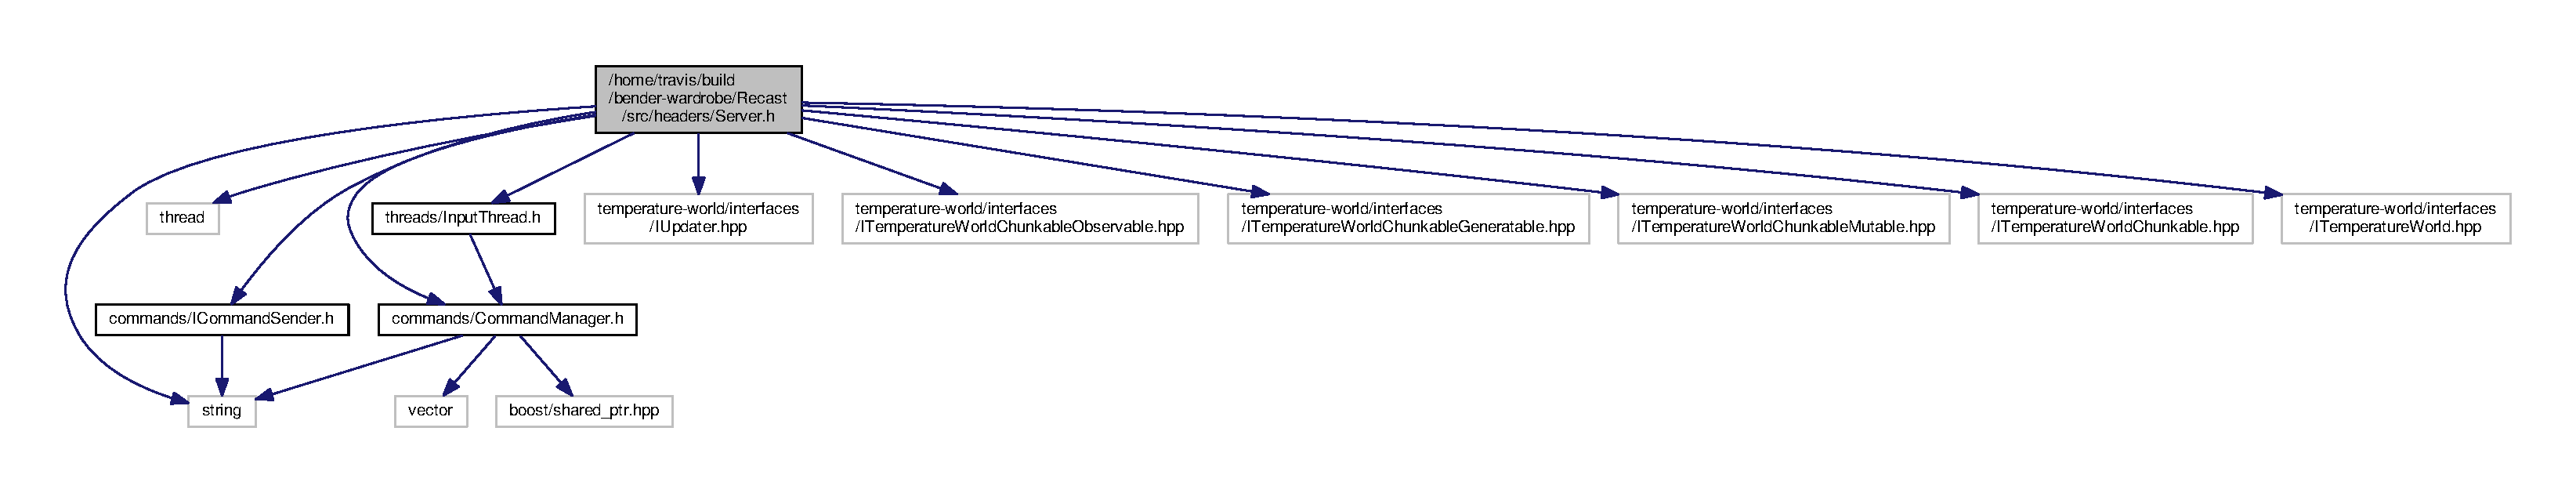
\includegraphics[width=350pt]{_server_8h__incl}
\end{center}
\end{figure}
This graph shows which files directly or indirectly include this file\-:
\nopagebreak
\begin{figure}[H]
\begin{center}
\leavevmode
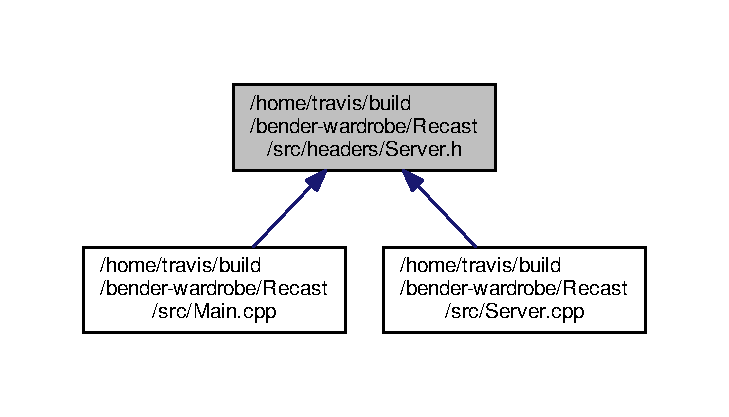
\includegraphics[width=350pt]{_server_8h__dep__incl}
\end{center}
\end{figure}
\subsection*{Classes}
\begin{DoxyCompactItemize}
\item 
class \hyperlink{class_server}{Server}
\begin{DoxyCompactList}\small\item\em Main class in Recast \hyperlink{class_server}{Server}. \end{DoxyCompactList}\end{DoxyCompactItemize}


\subsection{Detailed Description}
\hyperlink{class_server}{Server} file. \begin{DoxyAuthor}{Author}
Lion\-Z\-X\-Y  Recast 
\end{DoxyAuthor}
\begin{DoxyDate}{Date}
08.\-06.\-17
\end{DoxyDate}
Main server file (aka Context) 
\hypertarget{_main_8cpp}{\section{/home/travis/build/bender-\/wardrobe/\-Recast/src/\-Main.cpp File Reference}
\label{_main_8cpp}\index{/home/travis/build/bender-\/wardrobe/\-Recast/src/\-Main.\-cpp@{/home/travis/build/bender-\/wardrobe/\-Recast/src/\-Main.\-cpp}}
}


Starting point.  


{\ttfamily \#include $<$sqlite/src/sqlite3.\-h$>$}\\*
{\ttfamily \#include \char`\"{}Server.\-hpp\char`\"{}}\\*
Include dependency graph for Main.\-cpp\-:
\nopagebreak
\begin{figure}[H]
\begin{center}
\leavevmode
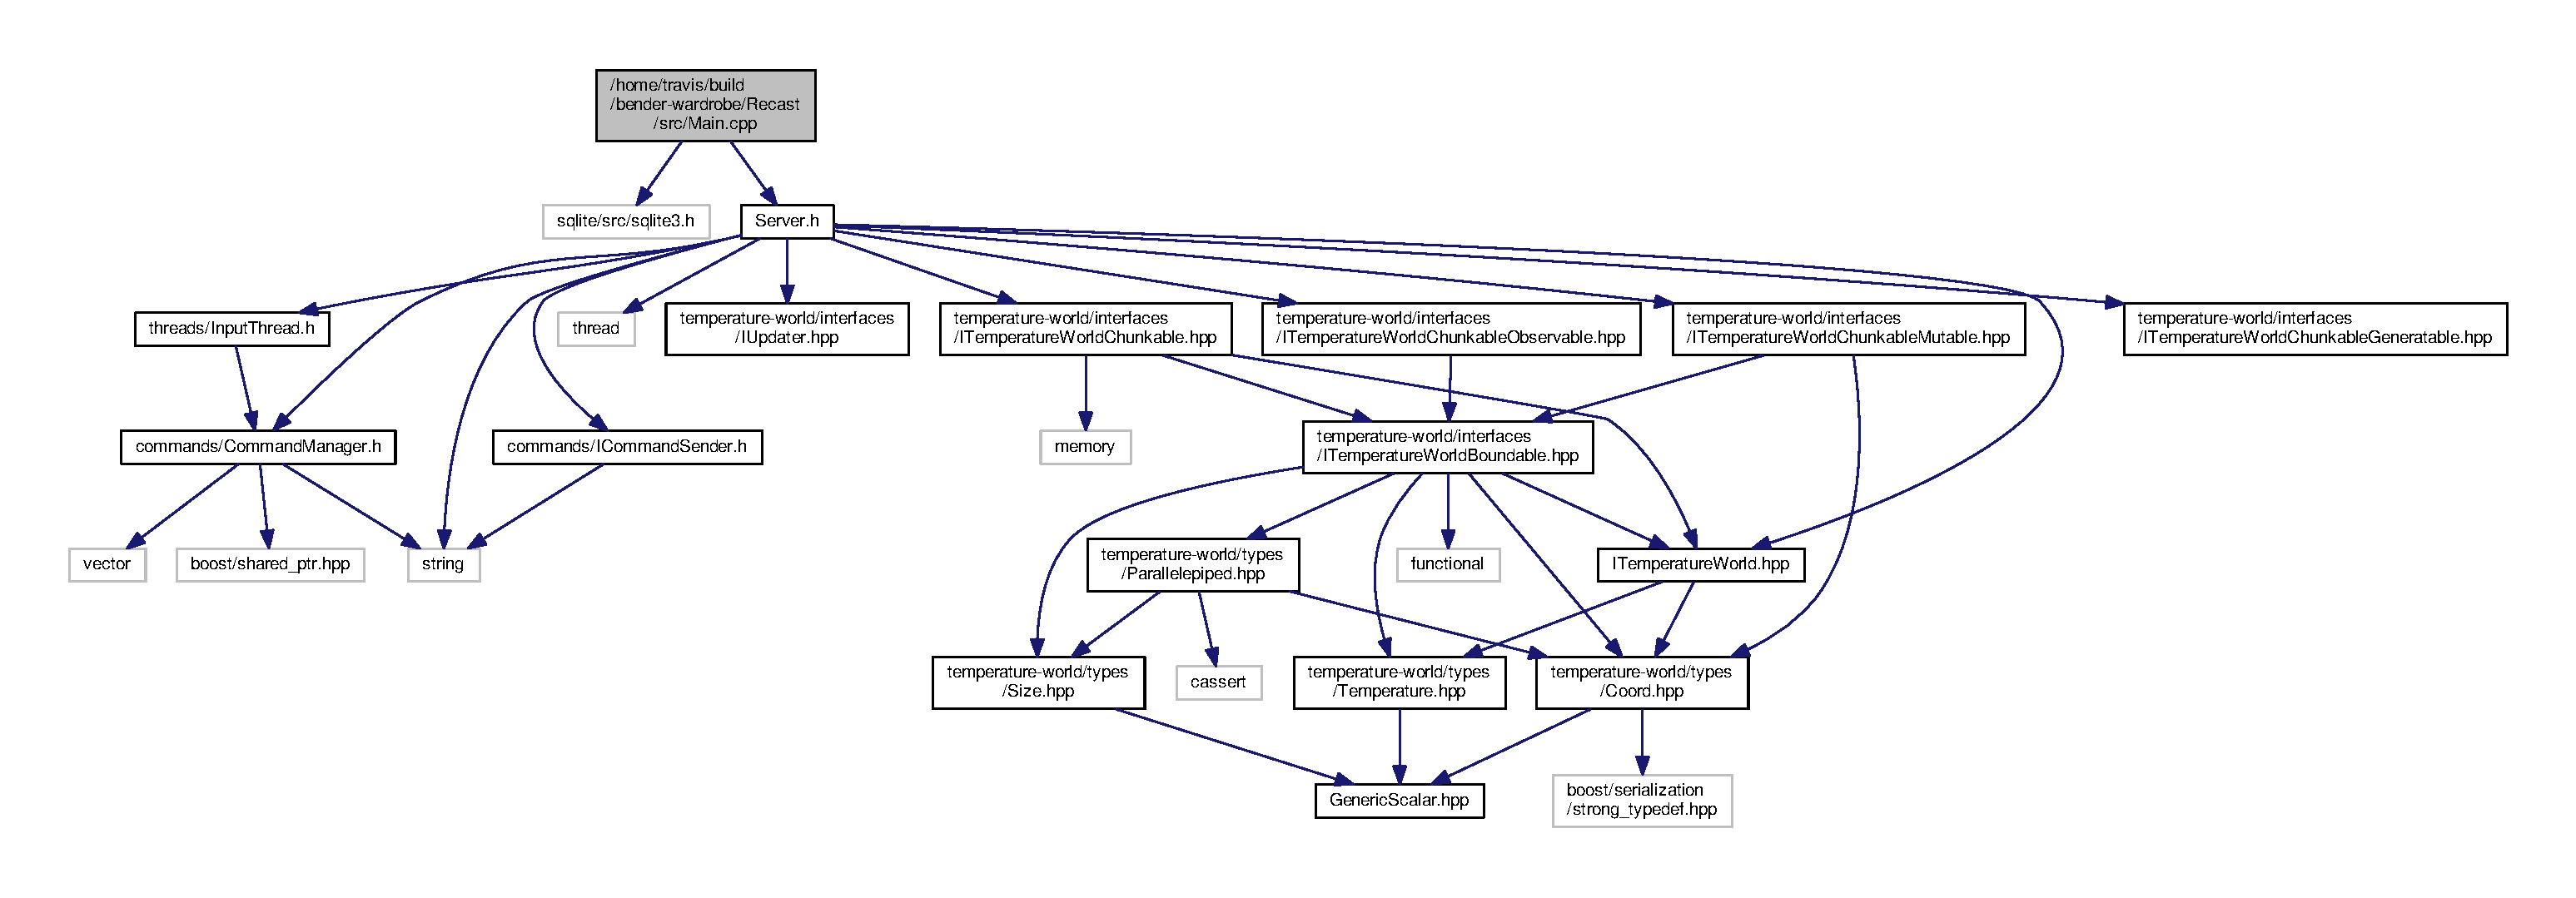
\includegraphics[width=350pt]{_main_8cpp__incl}
\end{center}
\end{figure}
\subsection*{Functions}
\begin{DoxyCompactItemize}
\item 
int \hyperlink{_main_8cpp_ae66f6b31b5ad750f1fe042a706a4e3d4}{main} ()
\begin{DoxyCompactList}\small\item\em Main method \-:) \end{DoxyCompactList}\end{DoxyCompactItemize}


\subsection{Detailed Description}
Starting point. \begin{DoxyAuthor}{Author}
Lion\-Z\-X\-Y
\end{DoxyAuthor}
Starting point for Recast server. Initializing \begin{DoxySeeAlso}{See Also}
\hyperlink{class_server}{Server} and 

Main\-Thread. Init config class 

\hyperlink{class_config}{Config}. 
\end{DoxySeeAlso}


\subsection{Function Documentation}
\hypertarget{_main_8cpp_ae66f6b31b5ad750f1fe042a706a4e3d4}{\index{Main.\-cpp@{Main.\-cpp}!main@{main}}
\index{main@{main}!Main.cpp@{Main.\-cpp}}
\subsubsection[{main}]{\setlength{\rightskip}{0pt plus 5cm}int main (
\begin{DoxyParamCaption}
{}
\end{DoxyParamCaption}
)}}\label{_main_8cpp_ae66f6b31b5ad750f1fe042a706a4e3d4}


Main method \-:) 



Here is the call graph for this function\-:
\nopagebreak
\begin{figure}[H]
\begin{center}
\leavevmode
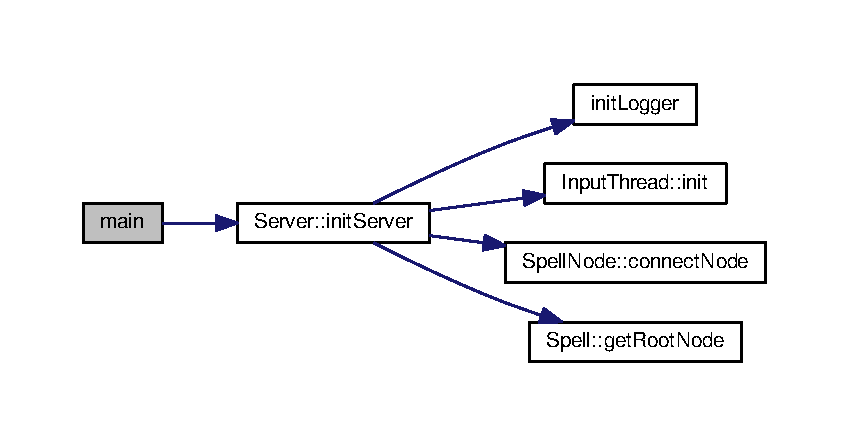
\includegraphics[width=350pt]{_main_8cpp_ae66f6b31b5ad750f1fe042a706a4e3d4_cgraph}
\end{center}
\end{figure}



\hypertarget{_server_8cpp}{\section{/home/travis/build/bender-\/wardrobe/\-Recast/src/\-Server.cpp File Reference}
\label{_server_8cpp}\index{/home/travis/build/bender-\/wardrobe/\-Recast/src/\-Server.\-cpp@{/home/travis/build/bender-\/wardrobe/\-Recast/src/\-Server.\-cpp}}
}


\hyperlink{class_config}{Config} file.  


{\ttfamily \#include $<$boost/log/trivial.\-hpp$>$}\\*
{\ttfamily \#include $<$boost/property\-\_\-tree/json\-\_\-parser.\-hpp$>$}\\*
{\ttfamily \#include $<$boost/log/expressions.\-hpp$>$}\\*
{\ttfamily \#include $<$boost/log/sinks/text\-\_\-file\-\_\-backend.\-hpp$>$}\\*
{\ttfamily \#include $<$boost/log/utility/setup/file.\-hpp$>$}\\*
{\ttfamily \#include $<$boost/log/utility/setup/common\-\_\-attributes.\-hpp$>$}\\*
{\ttfamily \#include $<$boost/log/utility/setup/console.\-hpp$>$}\\*
{\ttfamily \#include $<$boost/filesystem.\-hpp$>$}\\*
{\ttfamily \#include $<$exceptions/\-Invalid\-Login\-Or\-Password.\-h$>$}\\*
{\ttfamily \#include \char`\"{}io/\-S\-Q\-Lite.\-h\char`\"{}}\\*
{\ttfamily \#include \char`\"{}configs/\-Config.\-h\char`\"{}}\\*
{\ttfamily \#include \char`\"{}Server.\-h\char`\"{}}\\*
{\ttfamily \#include \char`\"{}threads/\-Input\-Thread.\-h\char`\"{}}\\*
{\ttfamily \#include \char`\"{}models/collections/\-Players\-Online.\-h\char`\"{}}\\*
Include dependency graph for Server.\-cpp\-:
\nopagebreak
\begin{figure}[H]
\begin{center}
\leavevmode
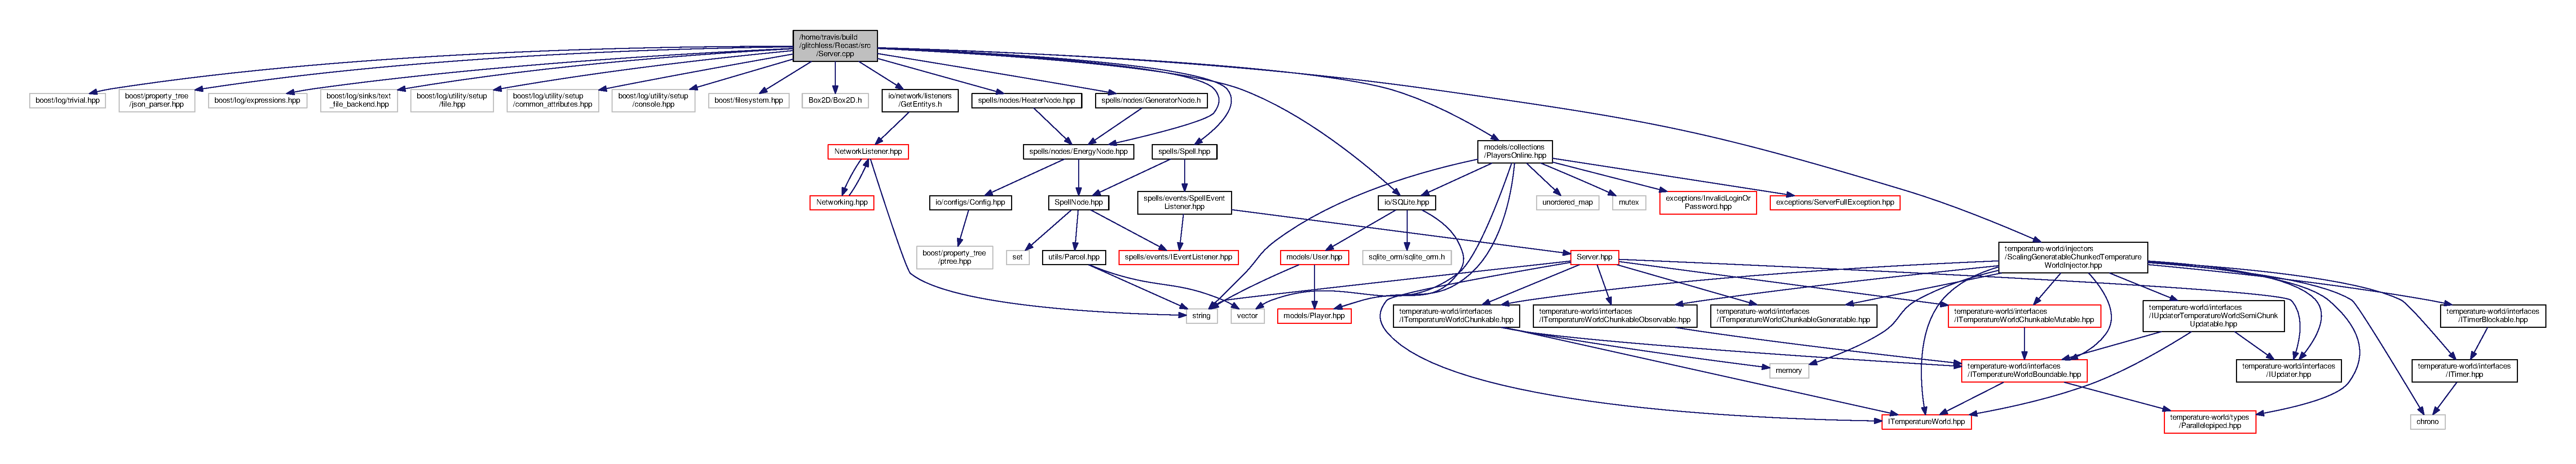
\includegraphics[width=350pt]{_server_8cpp__incl}
\end{center}
\end{figure}
\subsection*{Functions}
\begin{DoxyCompactItemize}
\item 
\hypertarget{_server_8cpp_a4fa9798662b6f85f704142579620acd0}{void {\bfseries init\-Logger} ()}\label{_server_8cpp_a4fa9798662b6f85f704142579620acd0}

\end{DoxyCompactItemize}


\subsection{Detailed Description}
\hyperlink{class_config}{Config} file. \begin{DoxyAuthor}{Author}
Lion\-Z\-X\-Y  Recast  \href{mailto:nikita@kulikof.ru}{\tt nikita@kulikof.\-ru} 
\end{DoxyAuthor}
\begin{DoxyDate}{Date}
08.\-06.\-17
\end{DoxyDate}
\hyperlink{class_server}{Server} file description 
\hypertarget{_player_8cpp}{\section{/home/travis/build/bender-\/wardrobe/\-Recast/src/world/models/\-Player.cpp File Reference}
\label{_player_8cpp}\index{/home/travis/build/bender-\/wardrobe/\-Recast/src/world/models/\-Player.\-cpp@{/home/travis/build/bender-\/wardrobe/\-Recast/src/world/models/\-Player.\-cpp}}
}


\hyperlink{class_player}{Player} file class.  




\subsection{Detailed Description}
\hyperlink{class_player}{Player} file class. \begin{DoxyAuthor}{Author}
Lion\-Z\-X\-Y  Recast-\/server 
\end{DoxyAuthor}
\begin{DoxyDate}{Date}
08.\-06.\-17
\end{DoxyDate}
\hyperlink{class_player}{Player} file class 
\hypertarget{_point_8cpp}{\section{/home/travis/build/bender-\/wardrobe/\-Recast/src/world/models/\-Point.cpp File Reference}
\label{_point_8cpp}\index{/home/travis/build/bender-\/wardrobe/\-Recast/src/world/models/\-Point.\-cpp@{/home/travis/build/bender-\/wardrobe/\-Recast/src/world/models/\-Point.\-cpp}}
}


\hyperlink{struct_point}{Point} file with some method.  




\subsection{Detailed Description}
\hyperlink{struct_point}{Point} file with some method. \begin{DoxyAuthor}{Author}
Lion\-Z\-X\-Y  Recast-\/server 
\end{DoxyAuthor}
\begin{DoxyDate}{Date}
08.\-06.\-17
\end{DoxyDate}
Now empty \-:3 
\chapter{Example Documentation}
\hypertarget{_on-example}{\section{On}
}
Run command. command 'stop now 1 2' from \hyperlink{class_server}{Server} console this method receives (\hyperlink{class_server}{Server}, 'stop'. \{'now','1', '2'\})

\begin{DoxyWarning}{Warning}
\hyperlink{class_i_command_sender}{I\-Command\-Sender} is N\-O\-T thread-\/safe. It means 
\end{DoxyWarning}

\begin{DoxyParams}{Parameters}
{\em sender} & is sent from background thread. If your \hyperlink{class_i_command}{I\-Command} needs main thread execution, create an issue. I will create a flag for that command.\\
\hline
{\em sender} & context object \\
\hline
{\em cmd} & first word in command \\
\hline
{\em args} & second and next words in command (Always not null)\\
\hline
\end{DoxyParams}

\begin{DoxyCodeInclude}
\end{DoxyCodeInclude}
 
\hypertarget{stop-example}{\section{stop}
}
call string command.\-Split string to arguments. Find command and run it.


\begin{DoxyParams}{Parameters}
{\em sender} & Link to any class who extend \hyperlink{class_i_command_sender}{I\-Command\-Sender}. Like \hyperlink{class_server}{Server}, \hyperlink{class_player}{Player} and other Context-\/like object. \\
\hline
{\em cmd} & Command in string. now.\\
\hline
\end{DoxyParams}

\begin{DoxyCodeInclude}
\end{DoxyCodeInclude}
 
%--- End generated contents ---

% Index
\newpage
\phantomsection
\addcontentsline{toc}{chapter}{Index}
\printindex

\end{document}
